\section{The ATLAS and CMS experiments} \label{sec:upgradelhc}

The planned upgrades to the ATLAS and CMS experiments for the HL-LHC will give the detectors increased coverage in the forward regions, better spatial and timing resolutions, and other new features including track triggers. The improved hardware capabilities, combined with software developments, give rise to exciting new prospects for future LLP searches. This section gives an overview of the upgrade scope (Section~\ref{sec:upgrademachine}), discusses their physics potential (Sections~\ref{sec:upgradeobject}-\ref{sec:upgradesearch}), and presents new ideas for detector upgrade and LLP searches (Section~\ref{sec:upgradeideas}).

Unless specified otherwise, the subsequent CMS experimental results are from its Technical Design Reports for the different sub-detector upgrades at HL-LHC, namely tracker~\cite{Collaboration:2272264}, barrel calorimeter~\cite{Lourenco:2283187}, endcap calorimeter~\cite{HGCal_TDR}, muon detectors~\cite{Lourenco:2283189}, timing detector (Technical Proposal, Ref.~\cite{MTD_TP}), and Level-1 Trigger (Interim Technical Design Report, Ref.~\cite{Lourenco:2283192}).

\subsection{Detector and Trigger Upgrades for High-Luminosity LHC} \label{sec:upgrademachine}

The High Luminosity LHC (HL-LHC) will begin with the third long shutdown (LS3) of the LHC in the coming decade (as of this writing estimated to begin at the end of 2023), where the machine and detectors will be upgraded to allow for pp running at a luminosity of $5 \times 10^{34}\,{\rm cm}^{-2}\,{\rm s}^{-1}$ in the nominal scenario, or potentially $7.5 \times 10^{34}\,{\rm cm}^{-2}\,{\rm s}^{-1}$ in the ultimate performance scenario. This will allow the ATLAS and CMS experiments to collect integrated luminosities ten times that of the current operations, which amounts to around $300$\fbinv~per year and $3000$\fbinv~during the projected HL-LHC lifetime of ten years (up to $4000$\fbinv if the ultimate instantaneous luminosity can be achieved).

The HL-LHC conditions create unique challenges in terms of high pile-up levels and high radiation dosage. About 140 pile-up events per bunch crossing, on average, are expected in the nominal scenario, and up to 200 pile-up events in the ultimate luminosity scenario. The radiation levels will be unprecedented:~for the design integrated luminosity of $3000$\fbinv, a $1$~MeV neutron equivalent fluence of $2.3 \times 10^{16}\,n_{eq}/{\rm cm}^2$ and a total ionizing dose (TID) of 12MGy (1.2 Grad) is expected at the centre of the detectors, where the innermost silicon pixel tracking layers will be installed.

To meet the challenges of the HL-LHC operating conditions, and to fully profit from its physics capabilities, comprehensive upgrade programmes are planned for both the ATLAS and CMS experiments. This section summarizes the main detector and trigger upgrade plans for each sub-detector component of both experiments.

\subsubsection{Tracker} \label{sec:upgradetracker}

%{\bf \textcolor{red}{[BS: For the benefit of laypeople, would it be helpful to have a picture showing pixels, strips, etc? since they come up for every detector?]}}

By the start of the HL-LHC, the inner trackers of both experiments must be replaced due to the significant radiation damage and performance degradation they have suffered. To maintain tracking performance in the high-density environment, and to cope with the increase of approximately a factor of ten in the integrated radiation dose, both the ATLAS and CMS experiments will entirely replace their inner tracking detectors.

\paragraph{CMS Upgrade}
The CMS tracker is composed of the inner pixel detector and the outer tracker. At the HL-LHC, the CMS inner pixel detector will include four cylindrical barrel layers covering the region of $|z| < 200$~mm, and forward extensions of up to twelve endcap disks on both sides (compared to the current configuration with three disks), which will extend its $|\eta|$ coverage from the current value of $2.4$ to approximately $4$. To maintain radiation hardness and reasonable occupancy, as well as to improve resolution, small, thin pixels will be used. For the studies in the CMS tracker TDR~\cite{Collaboration:2272264}, pixels with a thickness of $150\,\, \mu \mathrm{m}$ and $25\times100\,\,{\mu \mathrm{m}}^2$ in size are used in the simulation~\footnote{An alternative option being considered is that of $50\times50\,\,{\mu \mathrm{m}}^2$. Larger pixel sizes of $50\times200\,\,{\mu \mathrm{m}}^2$ or $100\times100\,\,{\mu \mathrm{m}}^2$ are being considered in outer barrel layers and outer rings of the endcap as a potential option to reduce power consumption.}.

The CMS outer tracker is composed of six cylindrical barrel layers in the central region, covering the region of $|z| < 1200$~mm, complemented on each side by five endcap double-disks, in the region of $1200 < |z| < 2700$~mm. Modules are installed between $r\sim21$~cm and $r\sim112$~cm. Three sub-detectors are distinguished:~the Tracker Barrel with pixel-strip modules (TBPS), the Tracker Barrel with strip-strip modules (TB2S), and the Tracker Endcap Double-Disks (TEDD). The inner rings of the TEDD disks use pixel-strip modules up to $r\sim 60$~cm, and the rest use strip-strip modules. The outer tracker modules, called $p_T$ modules, are composed of two single-sided, closely-spaced ($1$ to $4$~mm separation) small pitch sensors read out by a set of front-end ASICs that correlate the signals in the two sensors and select the hit pairs (referred to as ``stubs'') compatible with particles above the chosen $p_T$ threshold (see Fig.~\ref{fig:tracktrigger_toy}). A $p_T$ threshold of $2$~GeV corresponds to a data volume reduction of roughly one order of magnitude, which is sufficient to enable transmission of the stubs at 40~MHz.
The ``stubs'' are used as input to the hardware trigger at Level-1 (L1), which enables track-finding at L1 for all tracks with a $p_T$ of $2$~GeV or above. To improve the ``stub''-finding efficiency and also to reduce material, the inner three outer tracker barrel layers, the TBPS, are made with flat modules in the center and tilted modules in the regions with larger $z$.

\paragraph{ATLAS Upgrade}
The ATLAS collaboration will replace its inner detector with a new, all-silicon tracker to maintain tracking performance in HL-LHC conditions.

The new ATLAS Inner Tracker (ITk) will consist of a greatly enlarged pixel system extending to roughly twice the radius and four times the length of the current pixel array, coupled with a much more finely-segmented strip detector. In total, the coverage of the full radius of the inner solenoid requires over three times the silicon area of the current detector.

The new system will consist of silicon barrel layers and disks (strips) or rings (pixels) with the possibility of inclined pixel modules to better cover the transition from the barrel to the end-cap regions. In detail, the strip detector has four barrel layers and six end-cap petal-design disks, both having double modules each with a small stereo angle. The strip detector, covering $|\eta|< 2.7$, is complemented by a five-layer pixel detector extending the coverage to $|\eta |< 4$. The combined strip-plus-pixel detectors provide a total of 13 hits for $|\eta| < 2.6$, with the exception of the barrel/end-cap transition of the Strip Detector, where the hit count is 11.

\subsubsection{Calorimetry} \label{sec:upgradecalo}

Both the ATLAS and CMS calorimetry consist of electromagnetic calorimeters and hadronic calorimeters. Different materials and designs are used for the two experiments.

\paragraph{CMS Upgrade}
For the CMS detector, the existing scintillating crystals in its electromagnetic calorimeter (ECAL) barrel (EB) will be kept for the duration of LHC. On the other hand, both front-end and back-end electronics will be replaced~\cite{Lourenco:2283187}, which allows for higher transfer rates and more precise timing. The target timing resolution for the upgraded ECAL electronics is $\sim30$~ps for particles with $p_T \gtrsim30$~GeV, which is the fundamental limit allowed by hardware and an order of magnitude smaller than the current limit. Current studies on the CMS hadronic calorimeter (HCAL) barrel radiation damage suggest there is no need for replacement at HL-LHC.

The CMS endcap calorimeter, including both the electromagnetic (EE) and the hadronic sections, will be replaced with a high-granularity, silicon-based calorimeter (HGCAL). The HGCAL, with fine granularity in both the lateral and longitudinal directions, enables 3D imaging in reconstructing energy clusters. The intrinsic high-precision timing capabilities of the silicon sensors will add an extra dimension to event reconstruction. The HGCAL is expected to provide a timing resolution of $\sim10$s of ps for high-energy particles with $p_T$ of tens of GeV.

\paragraph{ATLAS Upgrade}

The ATLAS Liquid Argon (LAr) calorimeter will be improved in Phase-2 with an electronics upgrade that will provide optimized super cells and full-granularity data to the trigger system by means of a new pre-processor. A similar upgrade of the ATLAS Tile calorimeter readout will use on-detector digitization and a new backend pre-processor. Both the LAr and Tile calorimeters expect to implement a 40~MHz readout system for Phase-2. The transmission of high-granularity calorimeter data (all cells above a transverse energy threshold of $|E_T| > 2\sigma$) %{\bf \textcolor{red}{[JB: What does this mean? Energy in units of sigma?]}}
drives the bandwidth requirement for the upgraded trigger and data acquisition (TDAQ) system.

In addition, the outermost Tile calorimeter layer can be used to identify muons in the range $|\eta| < 1.3$ by better identifying particle energy depositions above the Minimum Ionizing Particle (MIP) threshold.

\subsubsection{Muon System} \label{sec:upgrademuon}

The muon system will be upgraded at both experiments to meet HL-LHC conditions, extend geometric coverage, and improve detector performance and trigger capabilities.

\paragraph{CMS Upgrade}

For the CMS detector, its current muon system consists of three different types of muon detectors. In the barrel region, drift tubes (DTs) are installed along with resistive plate chambers (RPCs). In the endcaps, there are cathode strip chambers (CSCs) together with RPCs. At the HL-LHC, the existing muon detectors will be improved with upgraded electronics to enable $40$~MHz readout, as well as improve the timing resolution from the current $12.5$~ns to $1$~ns~\cite{Lourenco:2283189}. New muon detectors, namely gas electron multipliers (GEMs) and a new version of RPCs, will be added to the endcaps, covering the regions of $1.6<|\eta|<2.4$. Additional muon chambers, labeled ME0, will cover the very forward regions of $2.4<|\eta|<2.8$, a region also covered by the upgraded inner tracker. This will be used for the muon trigger at L1. The additional muon detectors are essential to achieve a high trigger efficiency with an acceptable rate, especially in the forward region. The additional hits in the new endcap muon stations, combined with improved algorithms, permit efficient triggering on displaced muon tracks even in the harsh environment of the HL-LHC.

\paragraph{ATLAS Upgrade}

%{\bf \textcolor{red}{[BS: We are missing the ATLAS Trigger figure (hidden valley) in the MS section.]}}

Most of the front-end and detector readout of the ATLAS muon system, including the trigger electronics for the Resistive Plate Chambers (RPC), Thin Gap Chambers (TGC), and Monitored Drift Tube (MDT) chambers, will be replaced to face the higher trigger rates and longer latencies necessary for the new Level-0 (L0) trigger required by the HL-LHC conditions. The MDT chambers will be integrated into the L0 trigger in order to sharpen the momentum threshold. Some of the MDT chambers in the inner barrel layer will be replaced with new, small-diameter MDTs. Additional RPC chambers will be installed in the inner barrel layer to increase the acceptance and robustness of the trigger, and some chambers in high-rate regions will be refurbished. New TGC triplet chambers in the barrel--endcap transition region will replace the current TGC doublets to suppress the high trigger rate from random coincidences in this region. The electronics of all the sub-detectors will need to be replaced due to obsolescence, aging, and radiation damage. During the Phase-1 upgrade (to take place from 2019 to 2021) the New Small Wheel (NSW) chambers will replace the Cathode Strip Chambers (CSC) and the MDT chambers of the innermost endcap wheel by Micromegas and small-strip TGCs. The replacement of the MDT front-end readout will address the trigger rate and latency requirements of the TDAQ system in Phase-2 and allow the use of MDT hit information to improve the muon $p_T$ resolution in the L0 trigger.

Some LLP scenarios (e.g., Hidden Valley models~\cite{Strassler:2006im}) predict muon-jet final states, which result in collimated muons that are not identified with high efficiency by the current triggers (see Sec.~\ref{subsec:dleptons}). In Figure~\ref{fig:ATLAS_Trigger}, the opening angle between muons in a Hidden Valley model is shown, for a particular combination of particle masses and parameters. The di-muon separation is much smaller than the current system can resolve (approximately 0.2 in $\Delta\phi(\mu,\mu)$). In the no-upgrade scenario, these can only be recorded by the single muon trigger. In the upgraded scenario, a dedicated trigger is under development for a dimuon trigger with a $p_T$ threshold of $\approx$ 10 GeV.

\subsubsection{Timing Detector} \label{sec:upgradetiming}

Precision timing can be provided by the aforementioned calorimetry upgrades. However, the tens of ps timing resolution in the upgraded calorimeters is only achievable for particles with energy above tens of GeV. Moreover, timing information for delayed objects from calorimetry alone will be affected by the beamspot smearing, which corresponds to about $180$~ps of uncertainty. Therefore, global event timing with the ability to reconstruct the vertex time and exploit time information in charged particle reconstruction requires a dedicated fast timing detector.

\paragraph{CMS Upgrade}

For the CMS experiment, the proposed MIP timing detector (MTD) will comprise a barrel and an endcap region made up of a single layer device between the tracker and calorimeters, and cover $|\eta|$ up to $\sim3$. In the barrel, the proposal is to adapt the present Tracker Support Tube (TST) design by instrumenting the current location of the thermal screen with a thin, actively-cooled, standalone detector, based on lutetium-yttrium orthosilicate crystals activated with cerium (LYSO:Ce) and read-out with silicon photomultipliers. The endcap region can be instrumented with a hermetic, single layer of MIP-sensitive silicon devices with high timing resolution, with a pseudorapidity acceptance from about $|\eta|=1.6$ to $|\eta|=2.9$. The MTD is designed to provide timing resolution of a few tens of ps for charged tracks throughout the detector lifetime. The performance projection in Sec.~\ref{sec:upgradesearch} is evaluated with a 30~ps resolution for a $p_T$ threshold of 0.7 GeV in the barrel and a $p$ threshold of 0.7 GeV in the endcap, and covering the expected MTD fiducial region of $|\eta| < 3$.

\paragraph{ATLAS Upgrade}

The High-Granularity Timing Detector (HGTD) is intended to distinguish between collisions occurring very close in space but well-separated in time. Currently there is not yet a TDR for this project. The current proposed detector design is based on low-gain avalanche detector technology that will cover the $|\eta|$ region between 2.4 and 4,
with a timing resolution of 30~ps for MIPs. High-precision timing will improve the track-to-vertex association in the forward region, impacting jet and lepton reconstruction, as well as offering unique capabilities for online and offline luminosity determination.

\subsubsection{Trigger} \label{sec:upgradetrigger}

The ATLAS and CMS experiments adopt a two-level trigger system:~the hardware-based Level-1 trigger (L1) and the software-based high-level trigger (HLT). %{\bf \textcolor{red}{[JB: Do you mean that they each currently use a two-level trigger system and that this will continue for the Phase-2 upgrade? Above, in the section on muon systems, it's mentioned that ATLAS will have some kind of Level-0 trigger?  Can this be expanded a bit to give some context about triggering in ATLAS and CMS and how it's going to change?]}}
%{\bf \textcolor{red}{[JA: It's true at least for CMS that it currently uses at two-level trigger system and this will continue for the Phase-2 upgrade.]}}

\paragraph{CMS Upgrade}

For the CMS experiment, the L1 trigger currently only uses calorimeter and muon information. At the HL-LHC, with the aforementioned outer tracker upgrade of $p_T$ modules and stub-finding capabilities, tracking information will be included at L1~\cite{Lourenco:2283192}. The L1 track trigger uses parallel processing and pattern recognition on stub information to achieve track finding at an output rate of $750$~kHz.

The L1 tracking capability will be further complemented by the calorimeter and muon upgrades, which provide more precise position and momentum resolution, calorimeter shower shape, and more muon hits in the forward region. In the L1 trigger, the electron and photon trigger algorithms for HL-LHC will use information from the electromagnetic calorimeter as well as from the outer tracking detectors. The algorithm should preserve the ability to reconstruct electromagnetic clusters with $p_T$ above a few GeV with high efficiency ($95\%$ or greater above 10 GeV) as well as achieve high spatial resolution which should be as close as possible to the offline reconstruction. Following the upgrade of both on-detector and off-detector electronics for the barrel calorimeters at the HL-LHC, the EB %{\bf \textcolor{red}{[JB: What is the EB?]}} {\bf \textcolor{red}{[JA:The ecal barrel. EB was defined above.]}}
will provide energy measurements with a granularity of (0.0174, 0.0174)
in $(\eta, \phi)$, as opposed to the current input to the L1 trigger consisting of trigger towers with a granularity of (0.087, 0.087). The much finer granularity and resulting improvement in position resolution of the electromagnetic trigger algorithms is critical in improving electron/photon trigger efficiency and suppressing background at high pile-up.

The L1 Global Trigger (GT) will be upgraded with more sophisticated and effective global trigger calculations based on topology, plus an additional intermediate Correlator Trigger (CT) to fully exploit the increased information in the trigger objects, such as matching tracking info with finely-grained calorimeter information, or a combination of muon and track information. The upgraded detector readout and DAQ systems will allow $12.5\,\, \mu \mathrm{s}$ latency and a L1 rate of 750~KHz; the latter may be substantially reduced by adding L1 tracking information matched to improved L1 Calo and Muon trigger objects. At the high-level trigger (HLT), the processing power is expected to scale up by pile-up and L1 rate, with an output rate of $7.5$~kHz and up to $10$~kHz.

\paragraph{ATLAS Upgrade}

%{\bf \textcolor{red}{[JB: Can this section be expanded?  It would be great to provide a bit more detail about all of the things mentioned, to allow for a clearer comparison to the CMS plans.]}}

%\noindent {\bf \textcolor{red}{[BS: ATLAS L0 — it is mentioned earlier in the paper but it is not mentioned in the trigger section.]}}

%\noindent {\bf \textcolor{red}{[BS: ATLAS FTK doesn’t seem to be mentioned at all?]}}

The ATLAS trigger and the data acquisition system are being planned with the intention of fully exploiting the physics potential of the HL-LHC. A baseline architecture, based on a single-level hardware trigger with a maximum rate of 1~MHz and 10~$\mu$s latency, is proposed and documented in the aforementioned technical design documents. %{\bf \textcolor{red}{[BS: Reference?]}}
With the help of a hardware-based tracking sub-system as co-processor, software-based reconstruction follows to achieve further rejection. Up to 10~kHz event data are sent into storage.

The upgraded trigger system will take advantage of increased granularity provided by the calorimeters, will improve efficiency for muon-based triggers and perform hardware-based tracking profiting from the extended coverage of the planned Inner Tracker (ITk).

\subsection{Object Performance: Tracking and Vertexing} \label{sec:upgradeobject}

The ability of the detectors to reconstruct tracks and find vertices with high precision and efficiency in a high-density environment underlies the experimental reach for displaced objects. This section reviews the ATLAS and CMS experiments' projected tracking performance at the HL-LHC, highlighting improvements and new features with the upgrades.

\subsubsection{CMS Performance}

\paragraph{L1 Tracking}

With the aforementioned tracker and L1 track trigger upgrades, the CMS experiment will be able to do track finding at L1 as well as offline at HL-LHC. Both L1 and offline tracking performance are discussed here.

All L1 tracking studies have been performed assuming 3~GeV stub $p_T$ thresholds. In Figure~\ref{fig:cmsL1lepton}, the L1 tracking efficiency for prompt muons and electrons for \ttbar~events in a scenario with 200 pile-up interactions per bunch crossing, on average, is presented. The tracking efficiency for muons exhibits a sharp turn-on at the 3~GeV stub $p_T$ threshold, and saturates at approximately $98\%$. The tracking efficiency for electrons turns on more slowly and flattens out at $90\%$, mostly due to interaction with the detector material.

In Figure~\ref{fig:cmsL1tracks}, the L1 tracking resolutions of the $p_T$ and $z_0$ parameters of muons with $p_T > 10$~GeV in \ttbar~events is shown for various average pile-up scenarios. The resolutions are defined in terms of an interval centered on the residual distribution that contains $68\%$ or $90\%$ of the tracks. Loss in tracking efficiency due to truncation effects (where there is insufficient time to transfer all the stub data) is determined from hardware and emulation to be at the level of 10$^{-3}$ when considering \ttbar~samples with a pile-up rate of 200. As expected, resolutions degrade at forward pseudorapidity due to a corresponding increase in multiple scattering. In general, L1 parameter resolutions are excellent, which will provide for robust trigger object matching and charged particle reconstruction in the L1 trigger.

\begin{figure}[h!tbp]
\begin{center}
  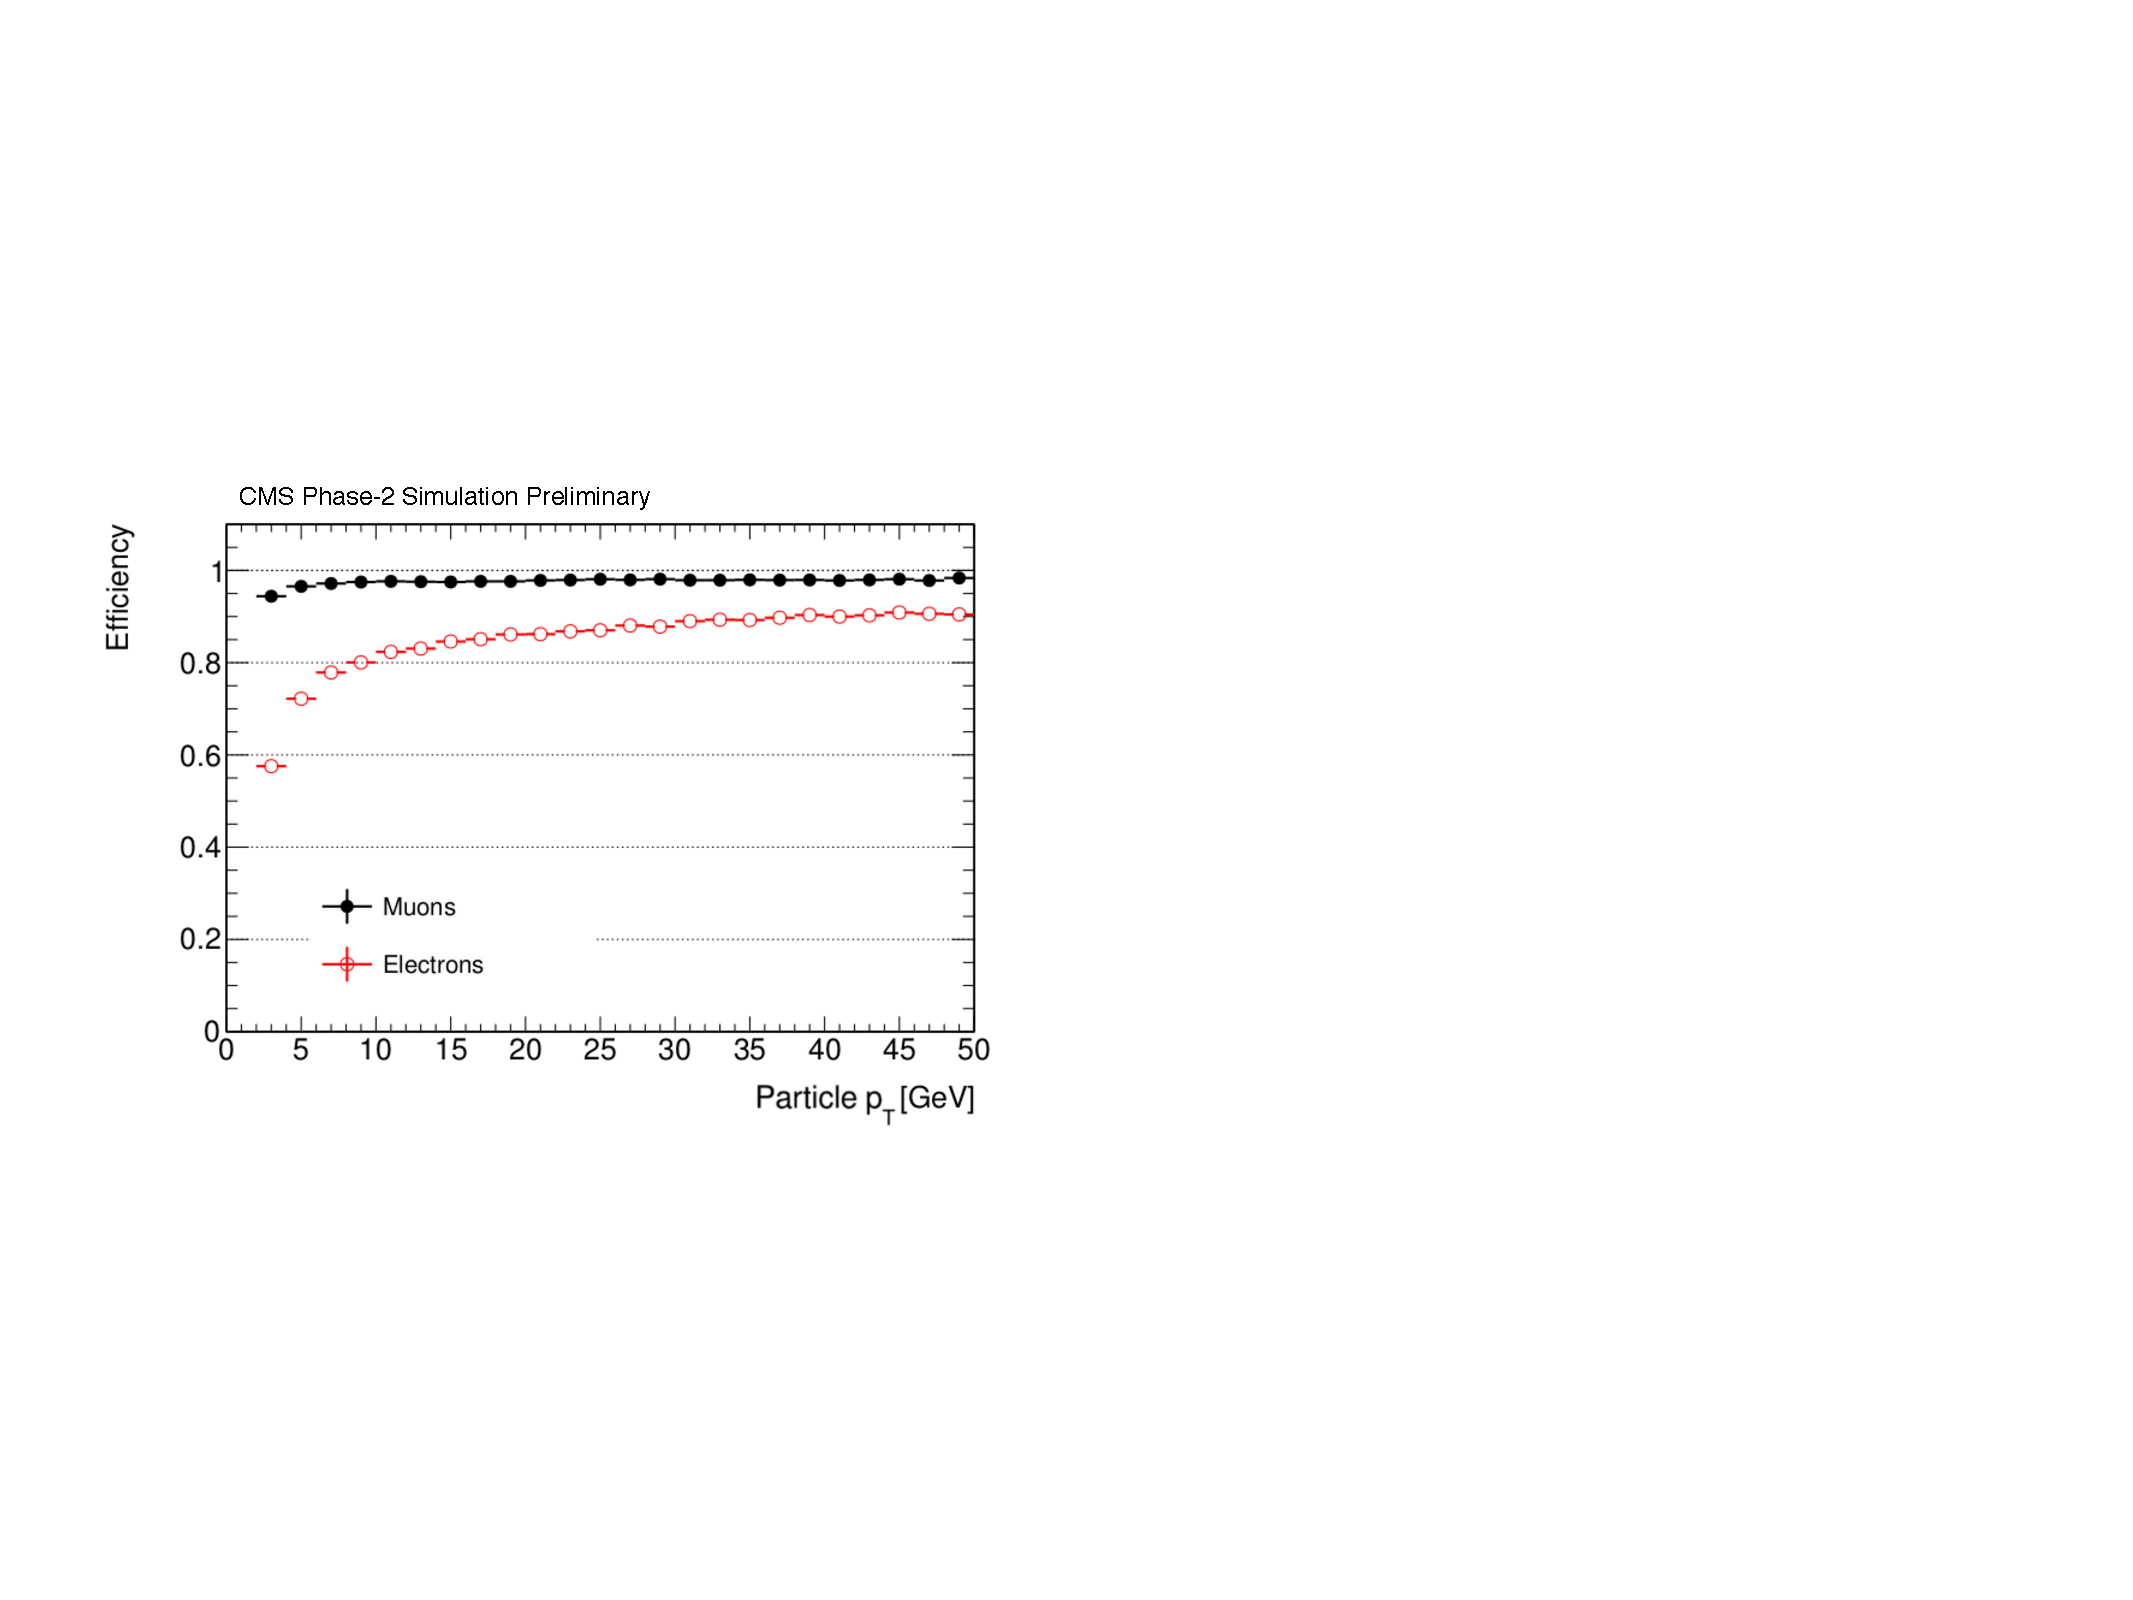
\includegraphics[width=0.47\textwidth]{figures/cmsupgrade/TDR-17-001_fig6_6_a.pdf} \hfill
  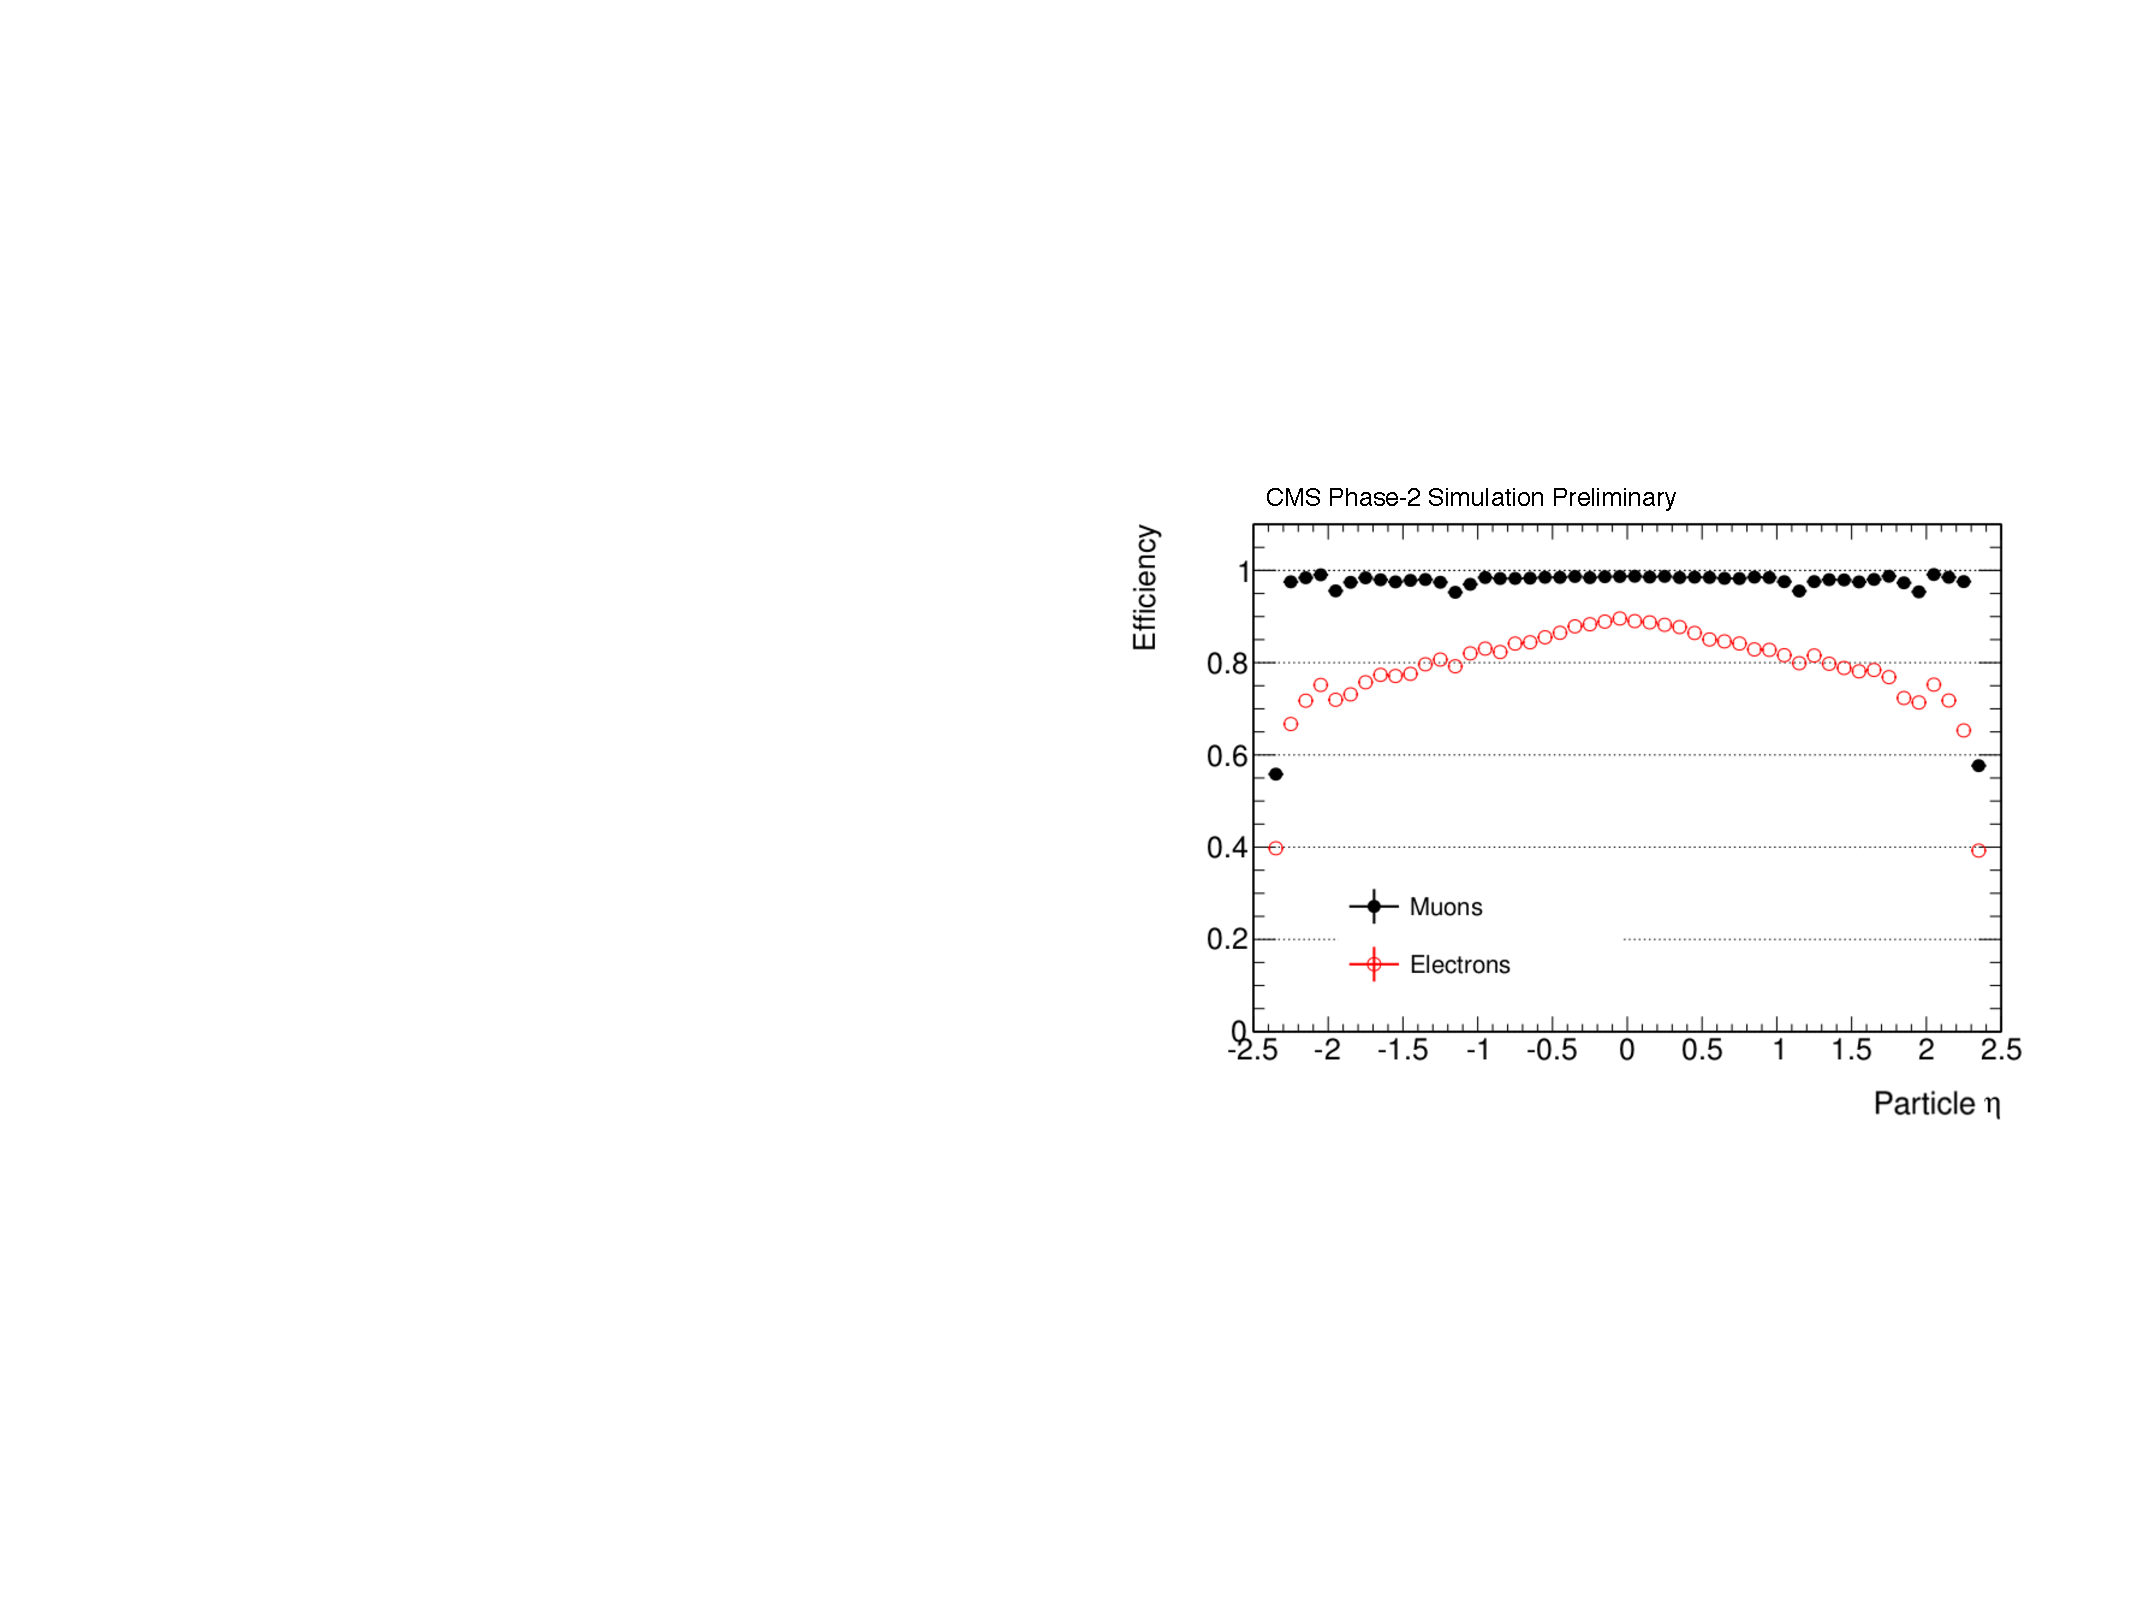
\includegraphics[width=0.47\textwidth]{figures/cmsupgrade/TDR-17-001_fig6_6_b.pdf}
  \caption{ Left:~L1 tracking efficiency versus generated particle $p_T$ for $|\eta| < 2.4$.
	Right:~L1 tracking efficiency versus $\eta$ for $p_T > 3$~GeV. Results for muons (electrons) are shown as filled black (open red) circles, and are produced with \ttbar~events in a scenario with 200 pile-up events per bunch crossing, on average. }
  \label{fig:cmsL1lepton}
\end{center}
\end{figure}

\begin{figure}[h!tbp]
\begin{center}
  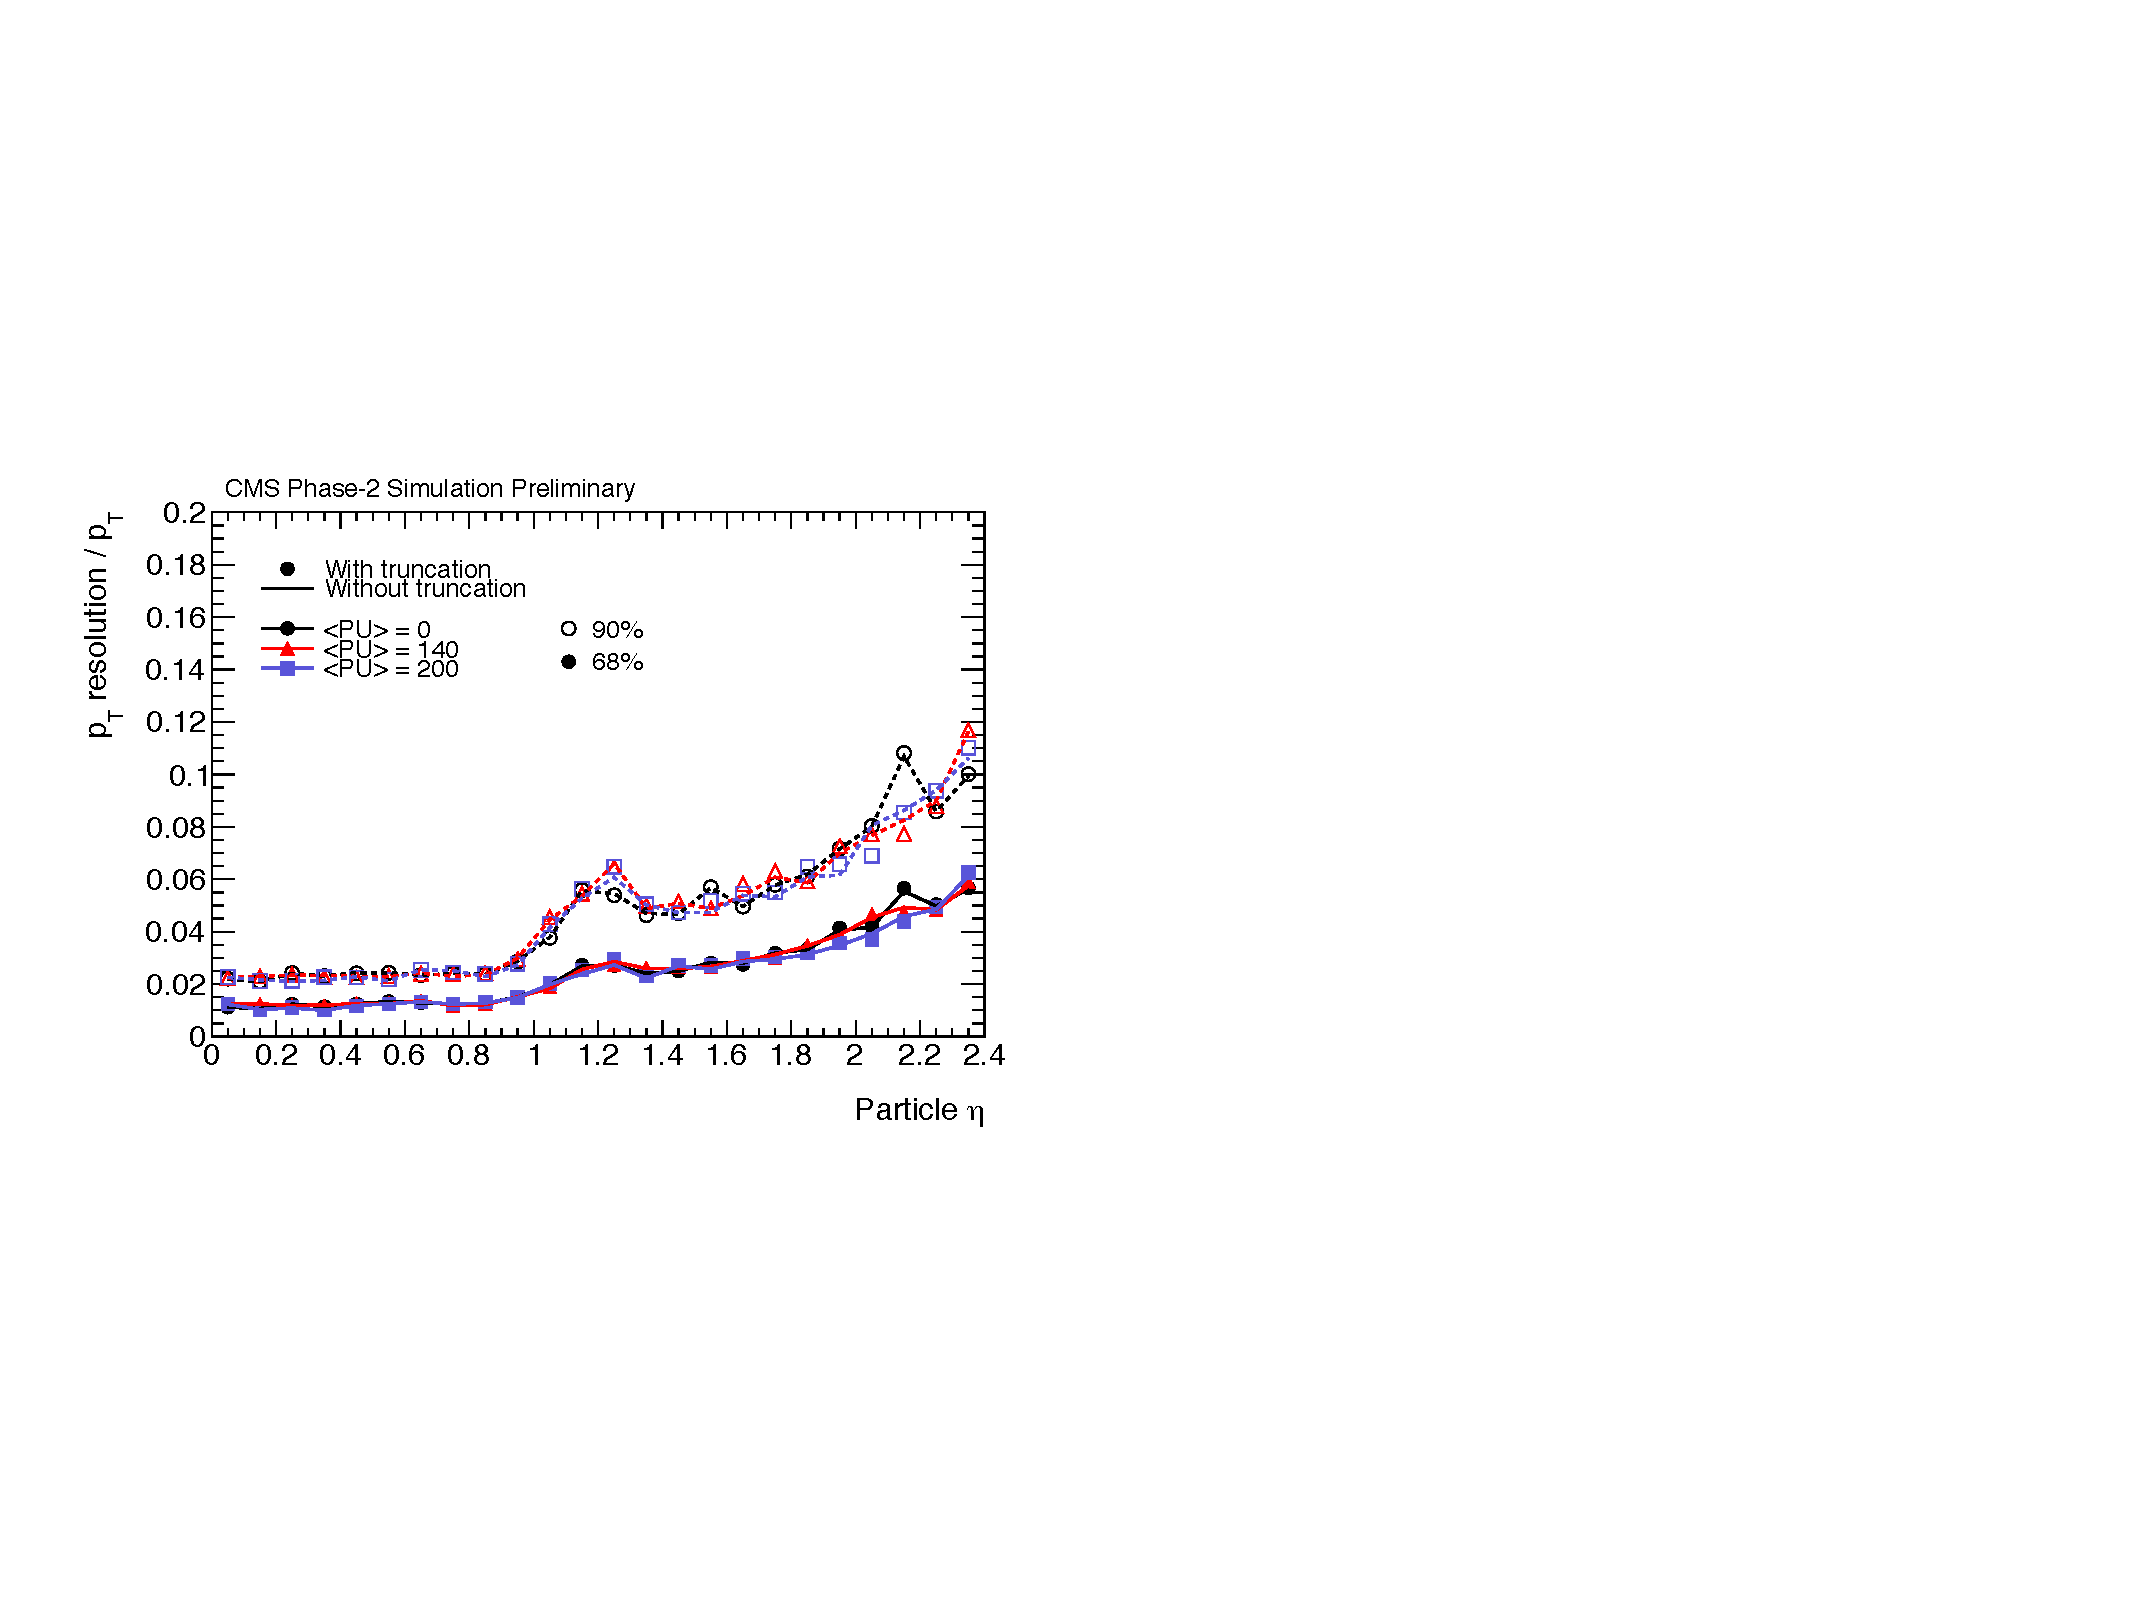
\includegraphics[width=0.47\textwidth]{figures/cmsupgrade/TDR-17-001_fig6_8_a.pdf} \hfill
  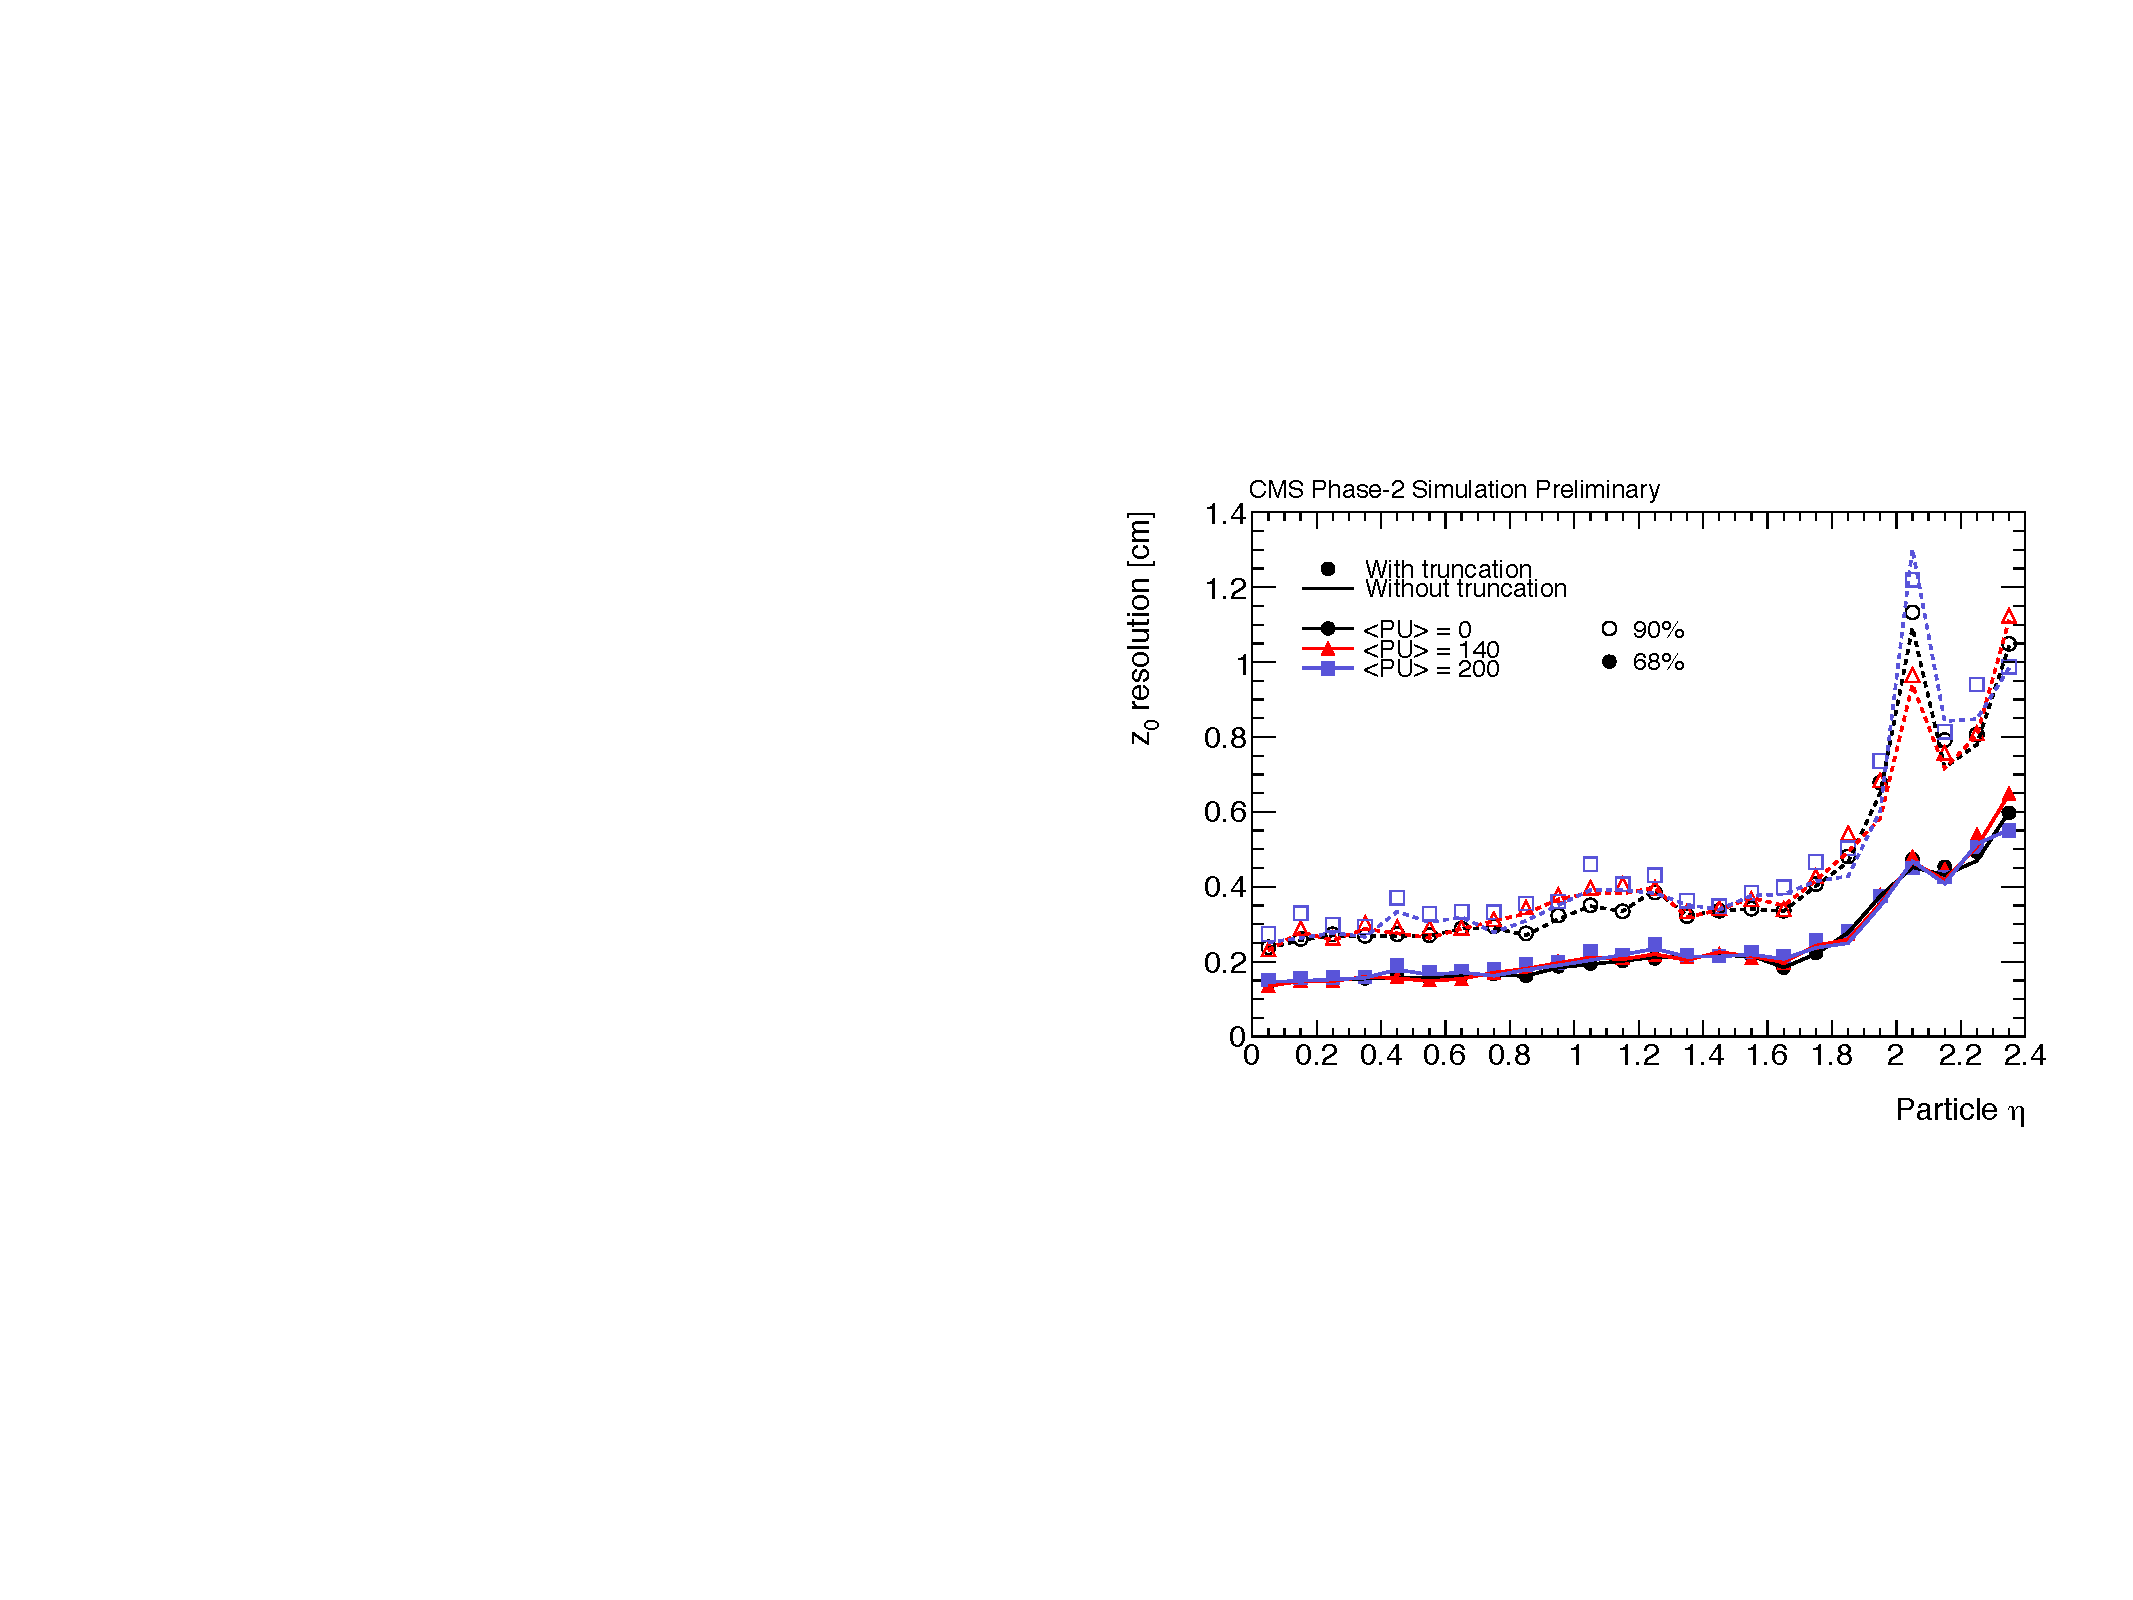
\includegraphics[width=0.47\textwidth]{figures/cmsupgrade/TDR-17-001_fig6_8_b.pdf}
  \caption{ Relative $p_T$ (left) and $z_0$ resolution versus pseudorapidity for muons in \ttbar~events with zero (black dots), 140 (red triangles), and 200 (blue squares) pile-up events per bunch crossing, on average. Results are shown for scenarios in which truncation effects are (markers) or are not (lines) considered in the emulation of L1 track processing. The resolutions correspond to intervals in the track parameter distributions that encompass $68\%$ (filled markers and solid lines) or $90\%$ (open markers and dashed lines) of all tracks with $p_T > 3$~GeV.}
  \label{fig:cmsL1tracks}
\end{center}
\end{figure}

\paragraph{Offline Tracking}

Preliminary results on the offline tracking performance over the full acceptance of the CMS tracker are excellent, with further improvements expected as the detector design and simulation algorithms are optimized. In Figure~\ref{fig:cmstrackres}, the resolution of the transverse momentum and the transverse impact parameter for single muons with $p_T = 10$~GeV as a function of the pseudorapidity, both with the current detector and after the implementation of the HL-LHC upgrades, is shown. The better hit resolution of the HL-LHC tracker and the reduction of the material budget result in a significantly improved $p_T$ resolution. The transverse impact parameter resolution is also improved with respect to the current detector, ranging from below $10\,\,\mu\mathrm{m}$ %{\bf \textcolor{red}{[BS: Should it be < 10 microns??]}} {\bf \textcolor{red}{[JA: Yes. Look at the figure below.]}}
in the central region to about $20\,\,\mu\mathrm{m}$ at the edge of the acceptance.

\begin{figure}[h!tbp]
\begin{center}
  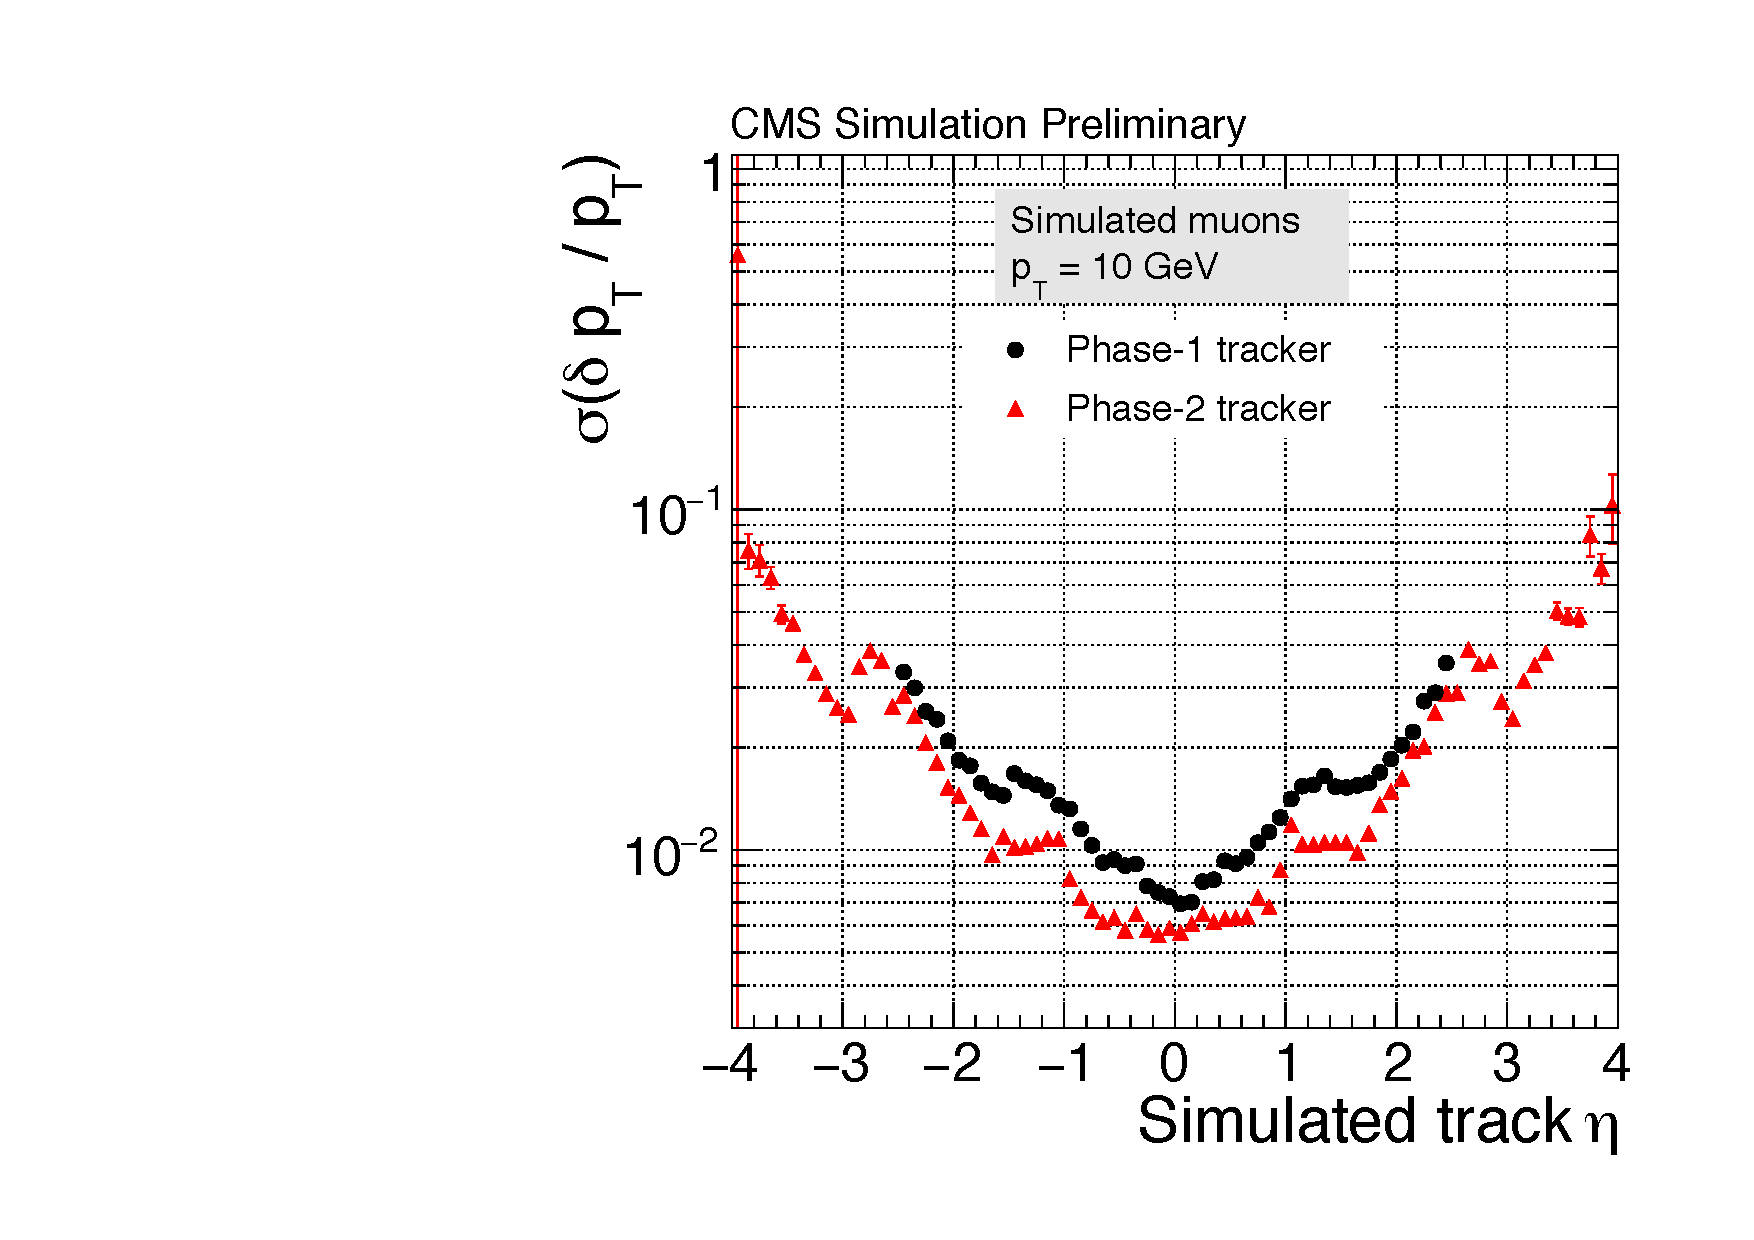
\includegraphics[width=0.47\textwidth]{figures/cmsupgrade/TDR-17-001_fig6_12_a_ptres_vs_eta_Sigma_vsPhase1.pdf} \hfill
  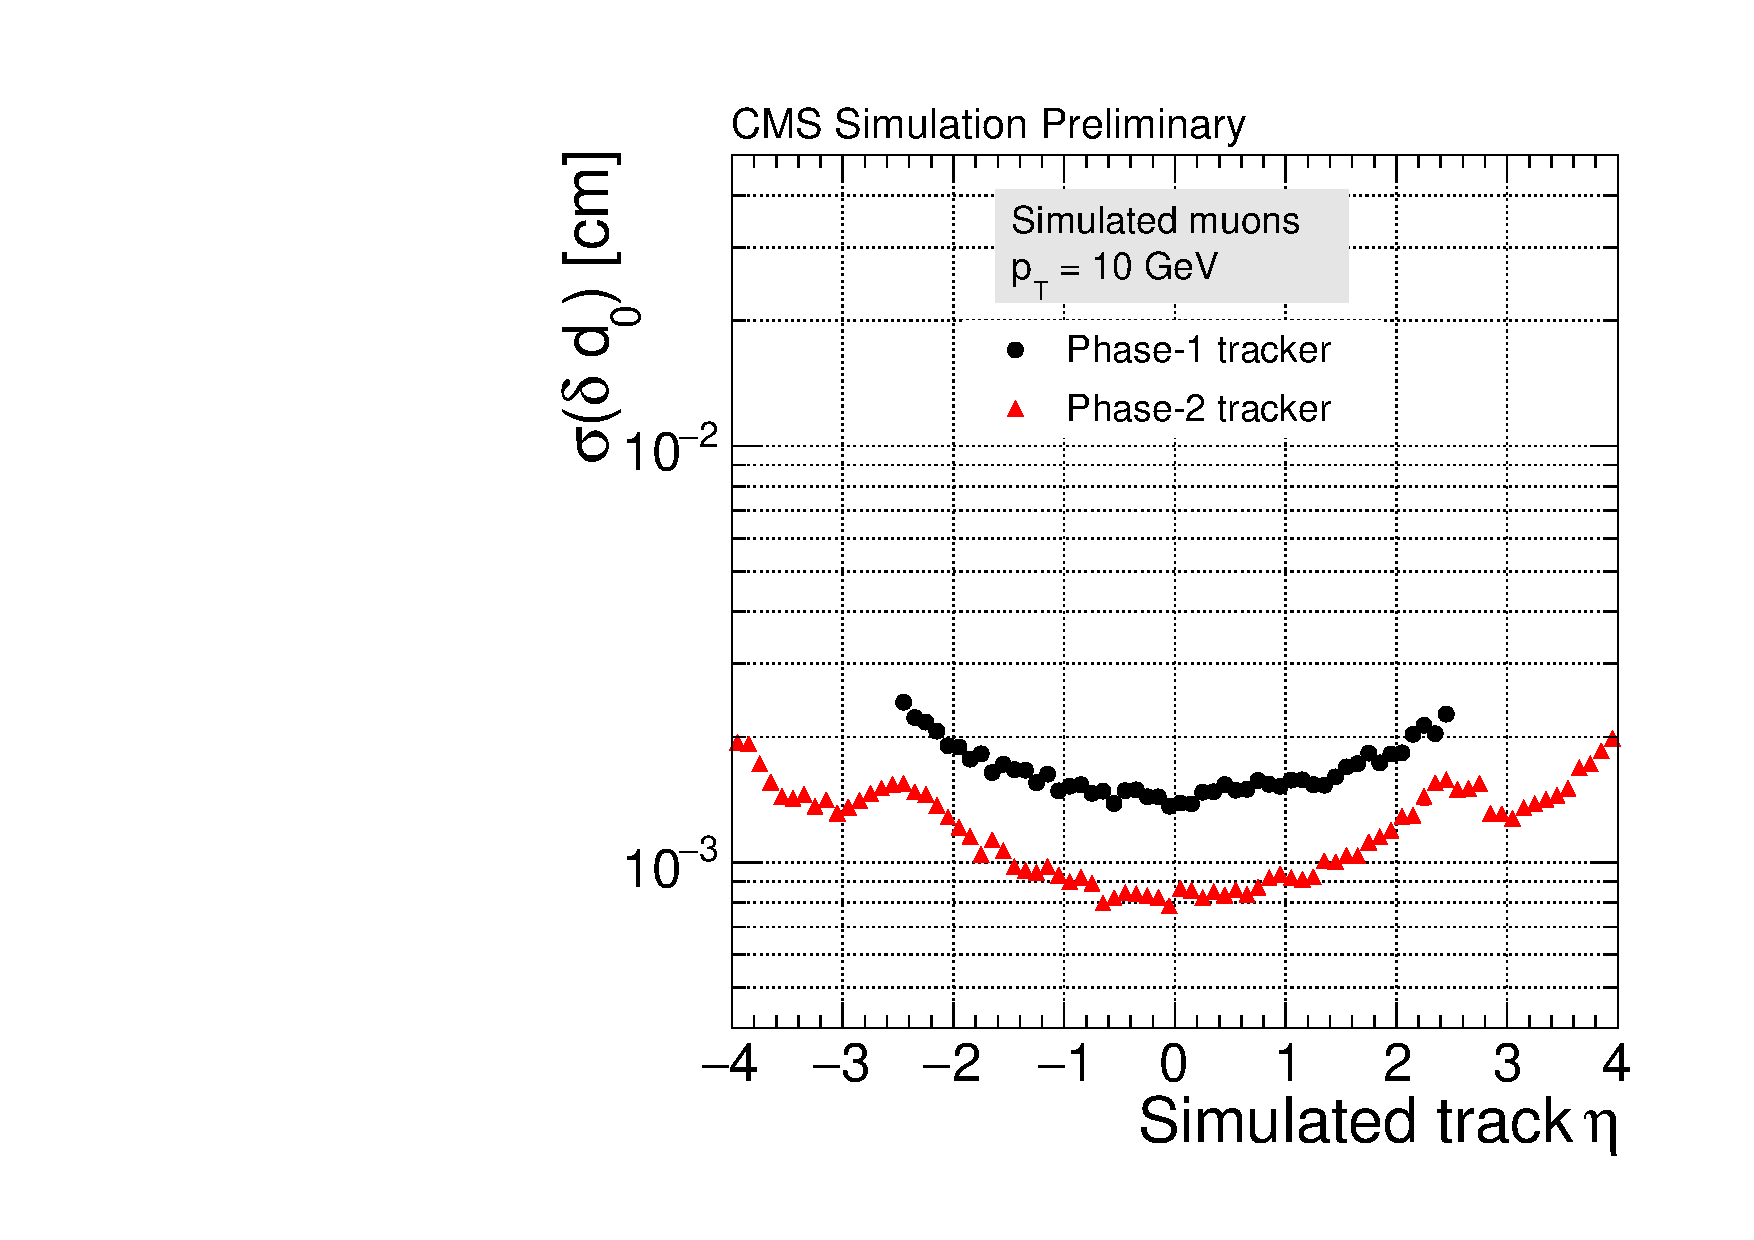
\includegraphics[width=0.47\textwidth]{figures/cmsupgrade/TDR-17-001_fig6_12_b_dxyres_vs_eta_Sigma_vsPhase1.pdf}
  \caption{Relative resolution of the transverse momentum (left) and transverse impact parameter (right) as a function of the pseudorapidity for the current (black dots) and the upgraded (red triangles) CMS tracker, using single isolated muons with a transverse momentum of $10$~GeV.}
  \label{fig:cmstrackres}
\end{center}
\end{figure}

For \ttbar~events, the efficiency to identify the primary vertex correctly is $\sim 95\%$ at an average pile-up level of 140, and $\sim93\%$ at an average pile-up level of 200. The vertex algorithm used is the same as the one used in Run 2 for a pile-up of about 35, therefore it is not yet optimized for vertex reconstruction at very high pile-up. In Figure~\ref{fig:cmsvertex} the resolution of the vertex position in the $x$, $y$, and $z$ coordinates is shown as a function of the number of tracks associated to the vertex. The vertex position resolution is almost independent of the amount of pile-up in the event and the longitudinal resolution is only $50\%$ worse than the transverse one, as expected given the pixel dimensions of the inner tracker modules.

\begin{figure}[h!tbp]
\begin{center}
  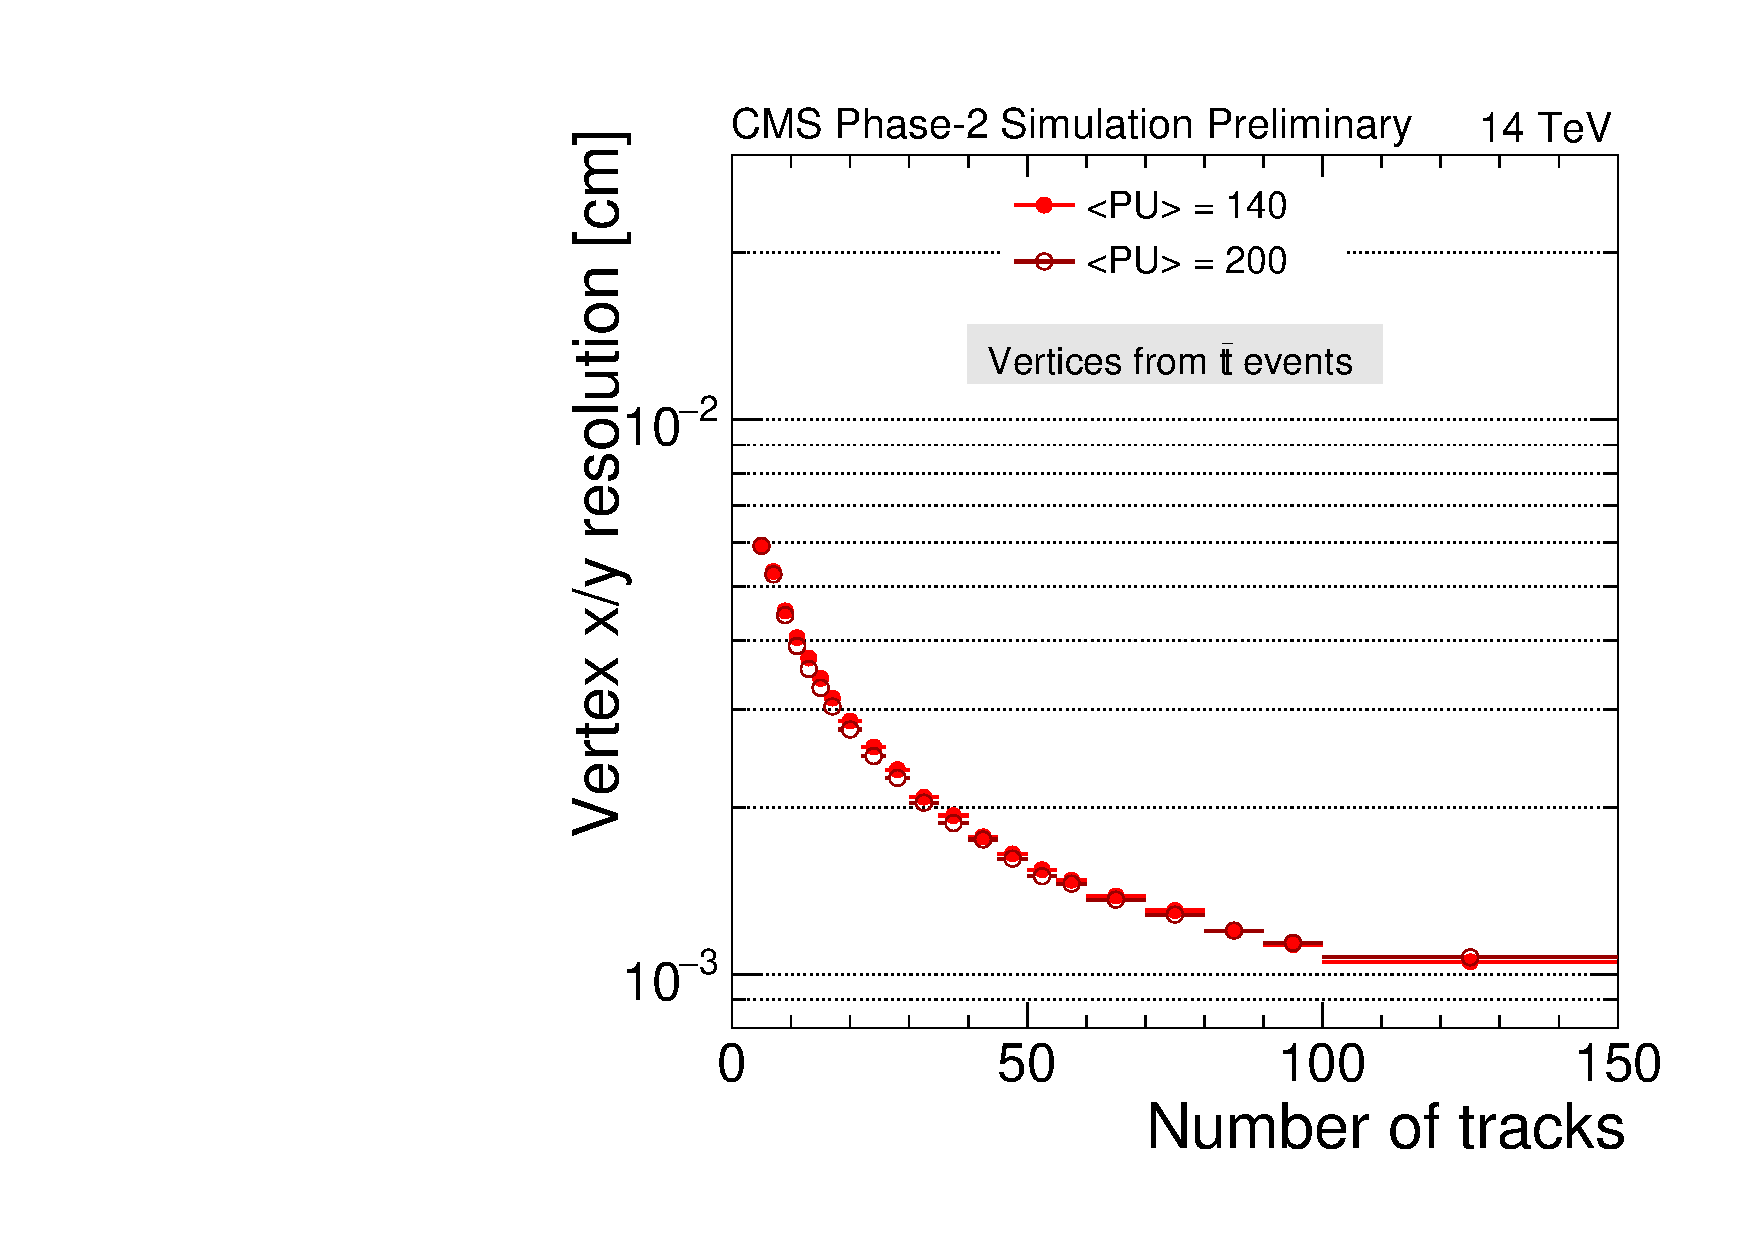
\includegraphics[width=0.47\textwidth]{figures/cmsupgrade/TDR-17-001_fig6_13_a_RecoAllAssoc2GenMatched_ResolX_vs_NumTracks_Sigma_PU.pdf} \hfill
  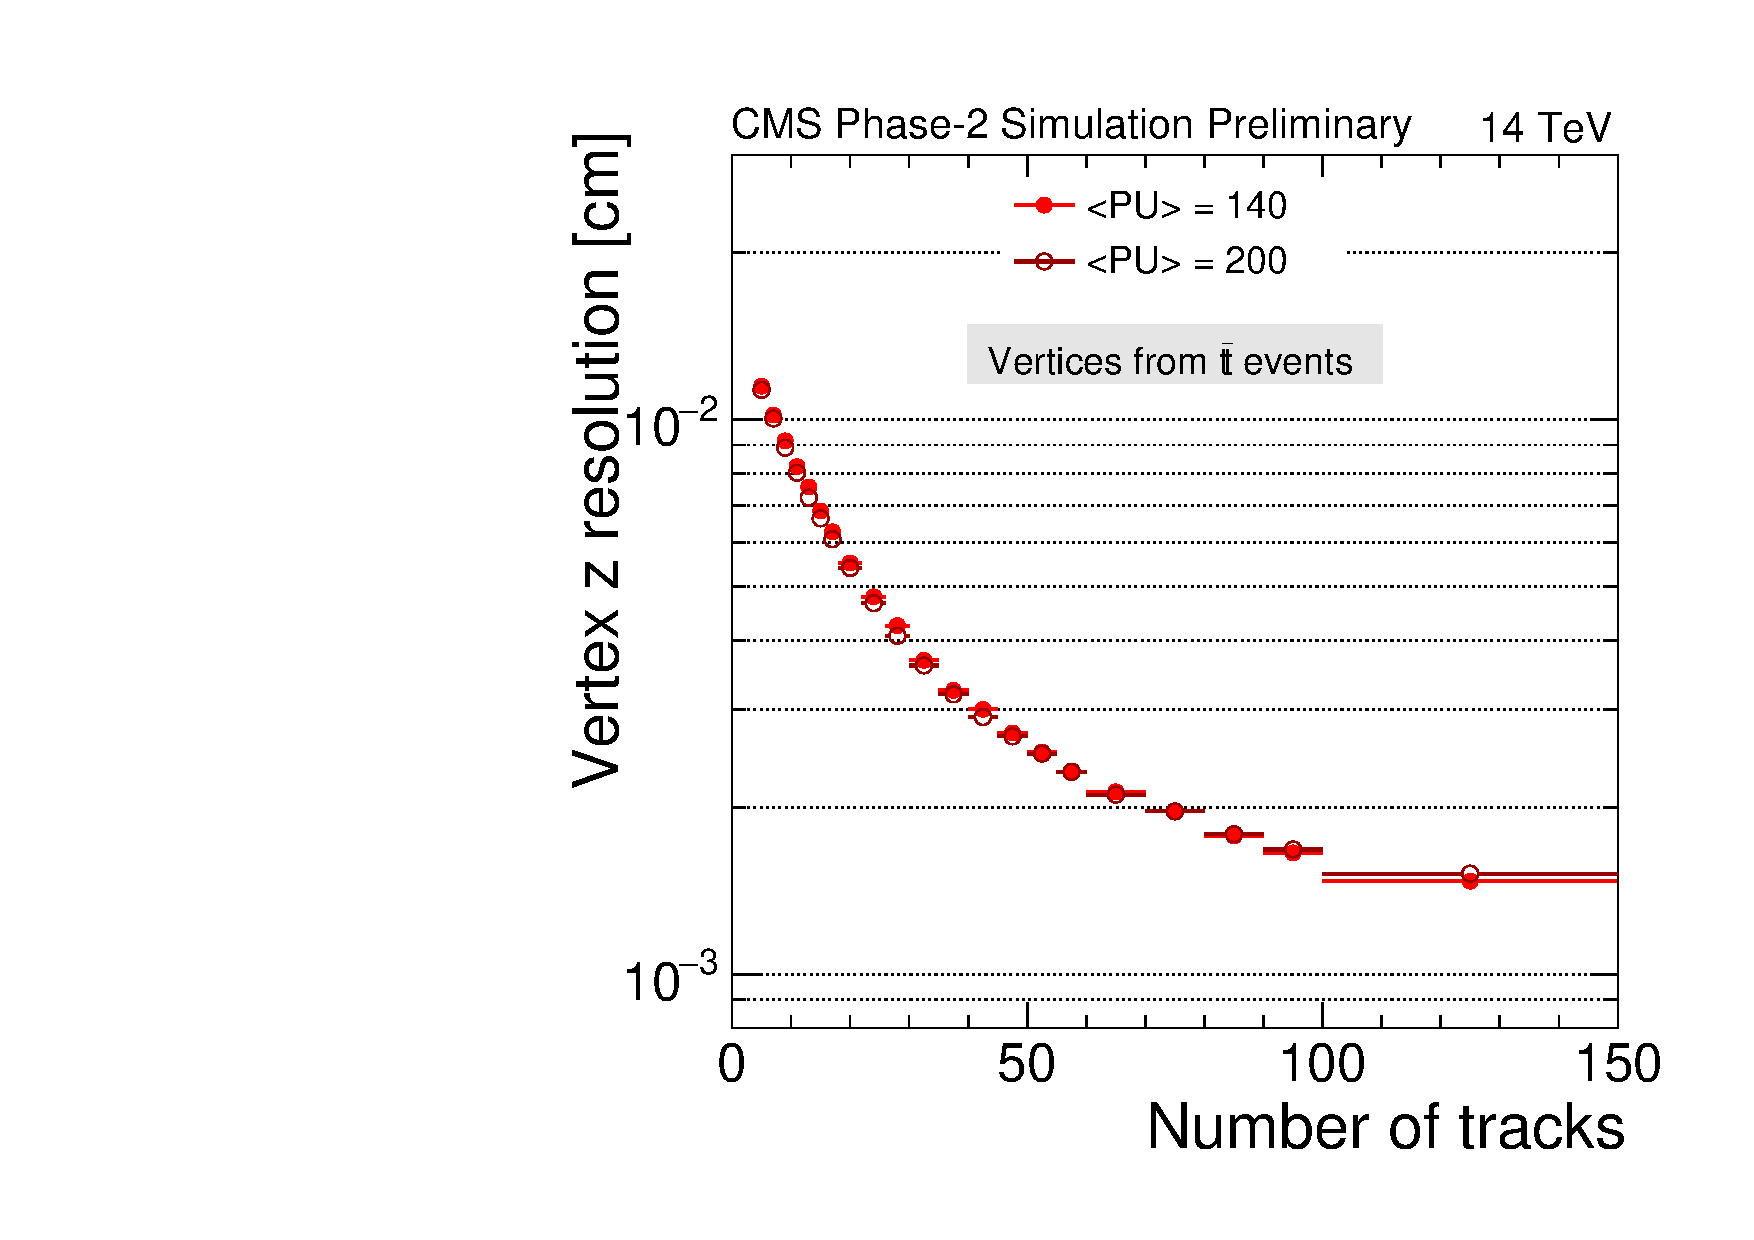
\includegraphics[width=0.47\textwidth]{figures/cmsupgrade/TDR-17-001_fig6_13_b_RecoAllAssoc2GenMatched_ResolZ_vs_NumTracks_Sigma_PU.pdf}
  \caption{Vertex position resolution in $x$ and $y$ (left) and $z$ (right) as a function of the number of tracks associated to the vertex, for \ttbar~events with an average of 140 (full circles) and 200 (open circles) pile-up interactions per bunch crossing.
 }
  \label{fig:cmsvertex}
\end{center}
\end{figure}

Given that the CMS HLT tracking is based on the offline tracking code, a similar level of performance is expected.
Because of HLT time constraints, a parallelization of the algorithms is already under development and will be applied also in the HLT track reconstruction at HL-LHC.

\subsubsection{ATLAS Performance}

%{\bf \textcolor{red}{[JB: It would also be great to expand this section a bit, to allow for a better comparison to the CMS section.]}}

%\noindent {\bf \textcolor{red}{[BS: Is there any additional tracking performance that can go here?]}}

Excellent tracking performance is also expected with the Inner Tracker (ITk) upgrade of the ATLAS experiment for the HL-LHC era.
%Figure~\ref{fig:atlastrackeff} shows the track reconstruction efficiency for jets in $Z'\to\ttbar$ events with 200 pile-up for different $\eta$ ranges.
In Figure~\ref{fig:atlastrackres}, the resolution of the transverse momentum and the longitudinal impact parameter for single muons with various $p_T$ values is shown as a function of the pseudorapidity both with the current
detector and projections for after the HL-LHC upgrade.

\begin{figure}[h!tbp]
\begin{center}
  
\includegraphics[width=0.47\textwidth]{figures/ch03_fig_006e.pdf}
  
\includegraphics[width=0.47\textwidth]{figures/ch03_fig_006b.pdf}
  \caption{Relative resolution of the transverse momentum (left) and longitudinal impact parameter (right) as a function of the pseudorapidity for the current (solid line) and the upgraded (points) ATLAS tracker.}
  \label{fig:atlastrackres}
\end{center}
\end{figure}

\subsection{Upgrade Projection: LLP Searches} \label{sec:upgradesearch}

%{\bf \textcolor{red}{[BS: Need to somehow organize performance studies — maybe separate sections for ATLAS and CMS?]}}

Searches for long-lived particles are well motivated by various classes of extensions of the Standard Model, discussed at length in Chapter~\ref{sec:motivated_theories}. Often, the production cross section for such processes is expected to be very small. The HL-LHC will allow for the collection of much larger data sets needed to reach better sensitivity to such BSM scenarios. The prospects are further strengthened with detector and trigger upgrades. This section discusses these potential improvements, and presents sensitivity projections on a number of benchmark LLP search channels with the aforementioned upgrades at the HL-LHC.

\subsubsection{Heavy Stable Charged Particles in CMS}

A number of new physics scenarios give rise to heavy stable charged particles (HSCPs) with long lifetimes that move with subrelativistical speed through the detector, heavily ionizing the sensor material as they pass through. In split SUSY models, the supersymmetric particles known as the stau ($\tilde{\tau}$) and the gluino ($\tilde{g}$) can have such characteristic signatures. The relevant simplified models are described in Secs.~\ref{sec:EMcharge}--\ref{sec:coloredLLPs}, and current searches are described in Sec.~\ref{subsec:ExpHSCP}.

\paragraph{Sensitivity projection with tracker upgrade}

Depending on the mass and charge of the new particles, HSCPs experience anomalously high energy losses through ionization ($dE/dx$) in the silicon sensors with respect to the typical energy losses of SM particles, as can be seen in Figure~\ref{fig:cmsupgrade_hscp} (left). At the CMS experiment, the current strip tracker features analog readout, and the pixel detector featured analog readout during Phase-0 in 2016 and before, and features digital readout during Phase-1, which was in place as of the beginning of the 2017 LHC run, allowing for excellent $dE/dx$ measurements.

At the HL-LHC, the upgraded CMS inner pixel detector will continue providing $dE/dx$ measurements, enabled by its time-over-threshold readout, while the outer tracker cannot provide such information, given that the readout is binary. To increase the sensitivity for signatures with anomalously high ionization loss, a second, programmable, threshold has been implemented in the short strip ASICs of the pixel-strip (PS) modules of the outer tracker, and a dedicated readout bit signals if a hit is above this second threshold.

Searches for HSCPs can thus be performed by measuring the energy loss in the inner pixel detector and by discriminating HSCPs from minimum ionizing particles based on the ``HIP flag'' in the outer tracker. The threshold of the minimum ionization needed to set the HIP flag is an adjustable parameter in each PS module independently. A threshold corresponding to the charge per unit length of 1.4 MIPs, resulting from preliminary optimization studies, is used in the simulation, and the gain in sensitivity obtained by using the HIP flag is studied.

An estimator of the degree of compatibility of the track with the MIP hypothesis is defined to separate candidate HSCPs from tracks from SM background sources. The high resolution $dE/dx$ measurements provided by the inner pixel modules are used for the computation of the $dE/dx$ discriminator. The tracks in background events have a low number of high threshold clusters with HIP flag, compared to those observed for tracks in HSCP signal events and slow-moving protons and kaons in minimum bias events.

In Figure~\ref{fig:cmsupgrade_hscp} (right), the performance of the discriminator is shown by evaluating the signal vs.~background efficiency curves to identify tracks from signal events and reject those originating from backgrounds. The performance curves are evaluated for two different strategies for the discriminator: the $dE/dx$ discriminator, which relies solely on the inner pixel modules ($dE/dx$-only, ignoring the HIP flags), and a recomputed discriminator which includes the HIP flags from the outer tracker PS modules ($dE/dx$ + HIP flags). The signal versus background efficiency performance curves demonstrate that for a background efficiency of $10^{-6}$, analogous to the current analysis performance, the $dE/dx+$HIP-based discriminator leads to an expected signal efficiency of $40\%$, around 4 to 8 times better than the $dE/dx$-only discriminator. In the $dE/dx$-only scenario, the efficiency for the HSCP signal is about 8 times smaller than that obtained in current data. The inclusion of the HIP flag for the PS modules of the Outer Tracker restores much of the efficiency, so that the same sensitivity as in Phase-1 will be realized with about four times the luminosity of Phase-1. The Phase-1 sensitivity will be surpassed with the full expected integrated luminosity of the HL-LHC. This study demonstrates the critical impact of the HIP flag in restoring the sensitivity of the CMS tracker for searches for highly ionizing particles in the HL-LHC era.

Additionally, the current CMS inner pixel detector provides measurements of charge deposits in each pixel up to $9,600$ electrons over a range of $4$-bits in the digitizer. While it may be difficult to increase the number of bits used to store the charge information due to data rate constraints, it is possible to adopt a dual-slope mapping from charge deposit to ADC counts in the digitizer, which will preserve the granularity for lower charge deposits, while giving more information for highly ionizing particles such as HSCPs. This option is currently being studied to evaluate the potential improvement to $dE/dx$ measurements. Furthermore, tuning of the HIP flag threshold may bring additional improvements.

\begin{figure}[t]
\begin{center}
  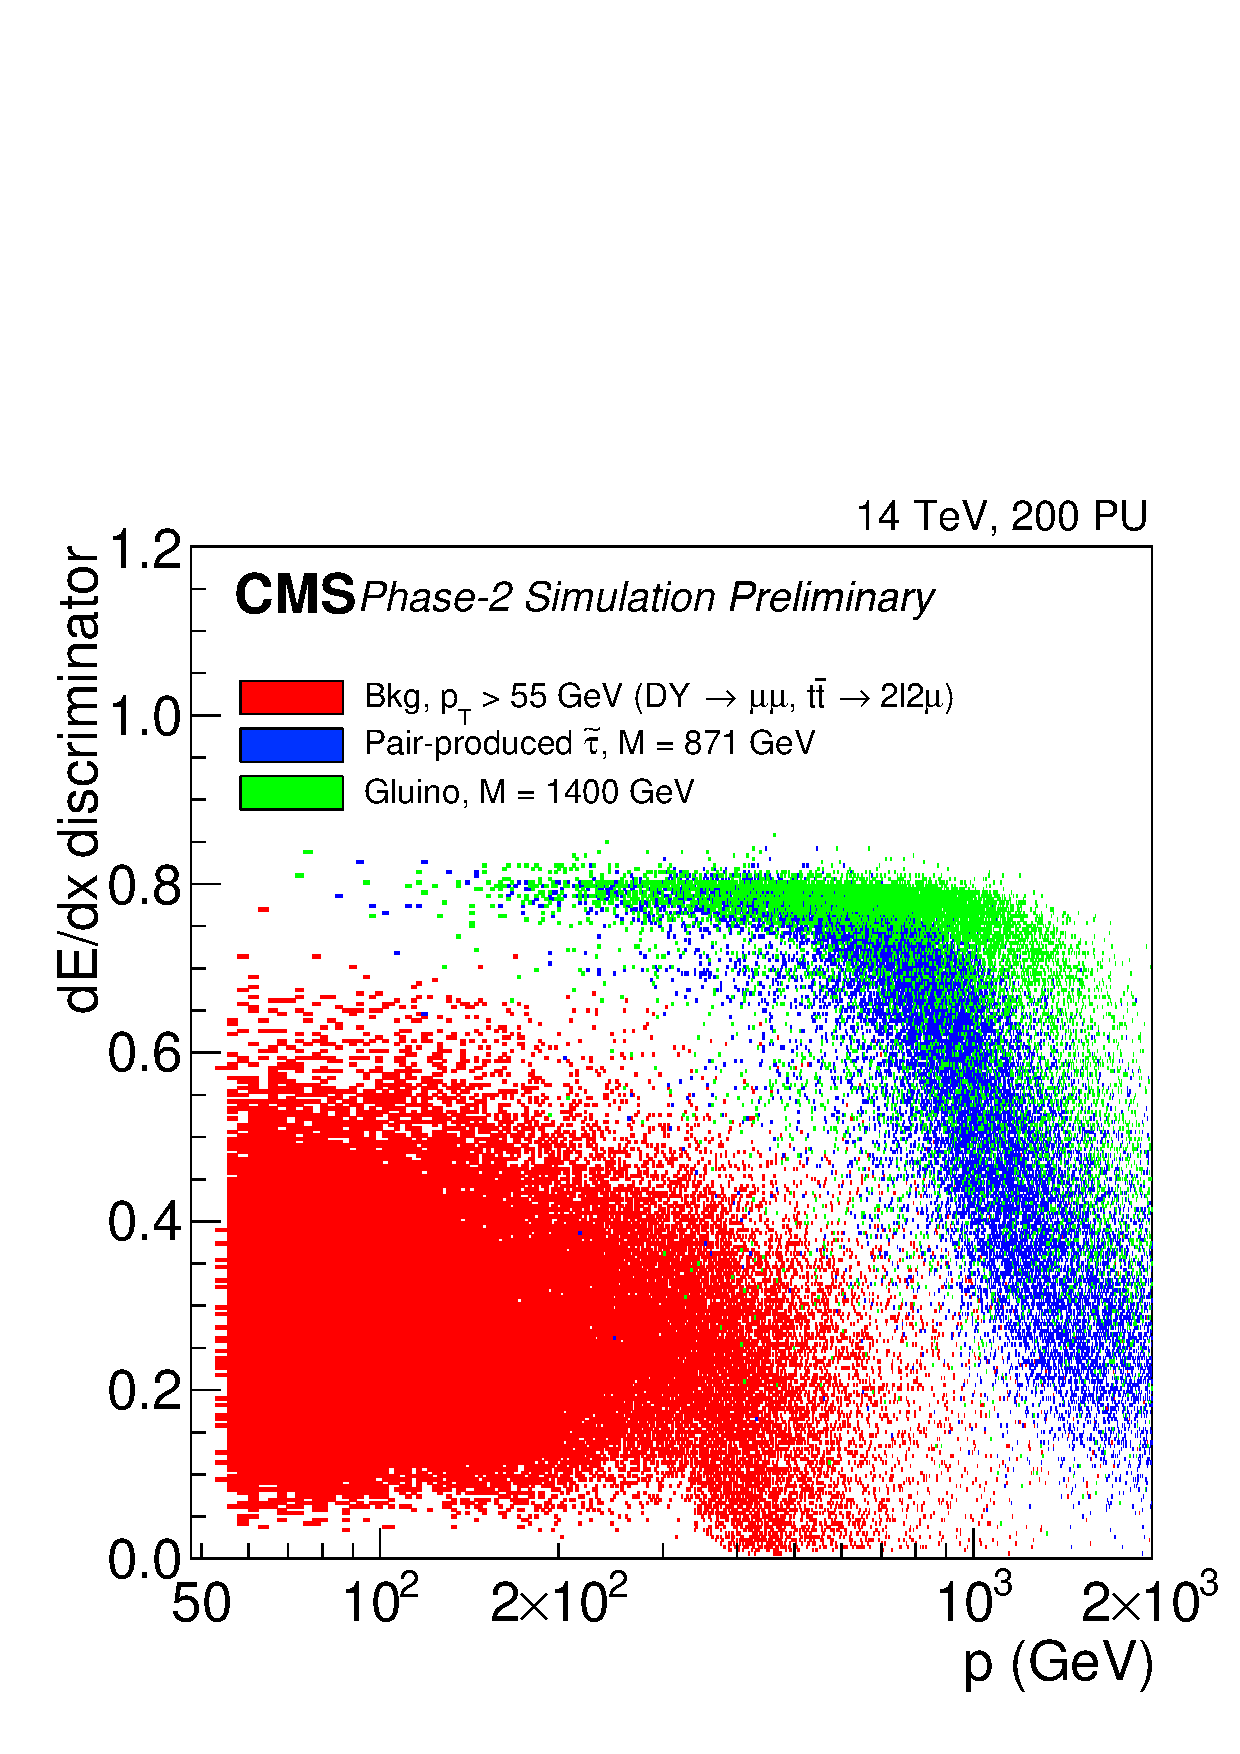
\includegraphics[width=0.47\textwidth]{figures/HSCP/TDR-17-001_fig6_26_a_HSCP_SpecialPlot_v2.pdf} \hfill
  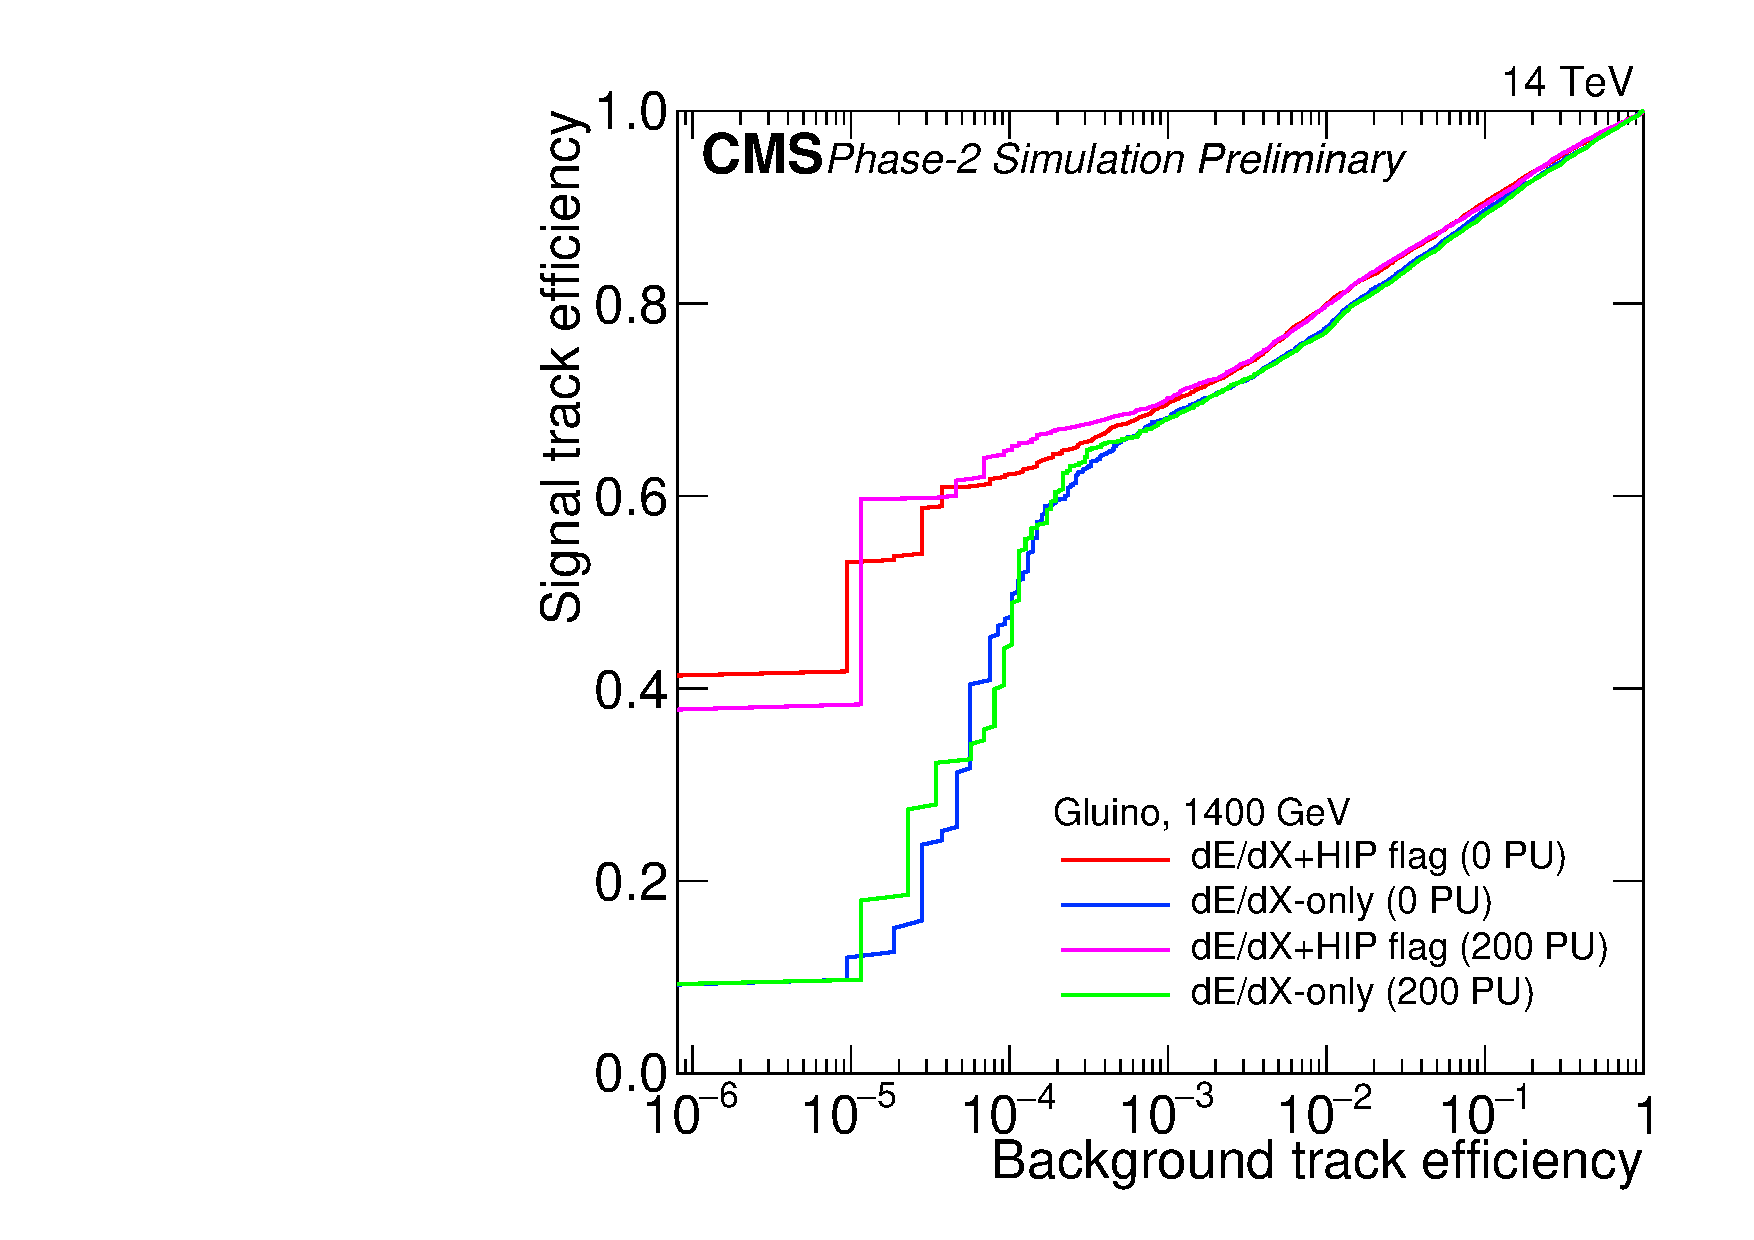
\includegraphics[width=0.47\textwidth]{figures/HSCP/TDR-17-001_fig6_27_a_HSCP_Comparison_ROC_Gluino_M1400_NoPU_Super_v2.pdf}
  \caption{Left:~Distribution in CMS of the $dE/dx$ discriminator versus track momentum ($p$) for tracks with high momentum ($p_T > 55$~GeV) in background events (red) and for candidate signal particles. Pair produced $\tilde{\tau}_S$ with a mass of 871~GeV (blue), and a gluino with a mass of 1400~GeV (green), are shown. Right:~The performance of the $dE/dx$ discriminator for selecting gluinos in events at rates of 0 pile-up (PU) and 200 PU. The signal vs. background efficiency performance curves for a discriminator making use of both the pixel information and the outer tracker HIP flag (red and magenta) demonstrate a better performance compared to a discriminator trained to exploit only the $dE/dx$ information from the pixel modules (blue and green), for a background rejection of $10^{-6}$.}
  \label{fig:cmsupgrade_hscp}
\end{center}
\end{figure}

\paragraph{HSCP trigger with muon detector upgrade}

The upgrade of the RPC system will allow the trigger and identification of slowly moving particles by measuring their time of flight to each RPC station with a resolution of $\mathcal{O}(1)$~ns. The speed of muon-like particles and the time (bunch crossing) of their origin will be computed with a fast algorithm to be implemented in the Level-1 trigger at the HL-LHC.

The RPC detectors are synchronized to register muons moving at the speed of light with a local time equal to zero with respect to the collision event that produced the trigger. Slow-moving particles, as HSCPs, will arrive with a delay depending on their speed as shown in Fig.~\ref{fig:hscp_time}. This time delay, measured by each RPC layer crossed by the HSCP, is exploited in order to trigger on and reconstruct such particles.

\begin{figure}[t]
\begin{center}
  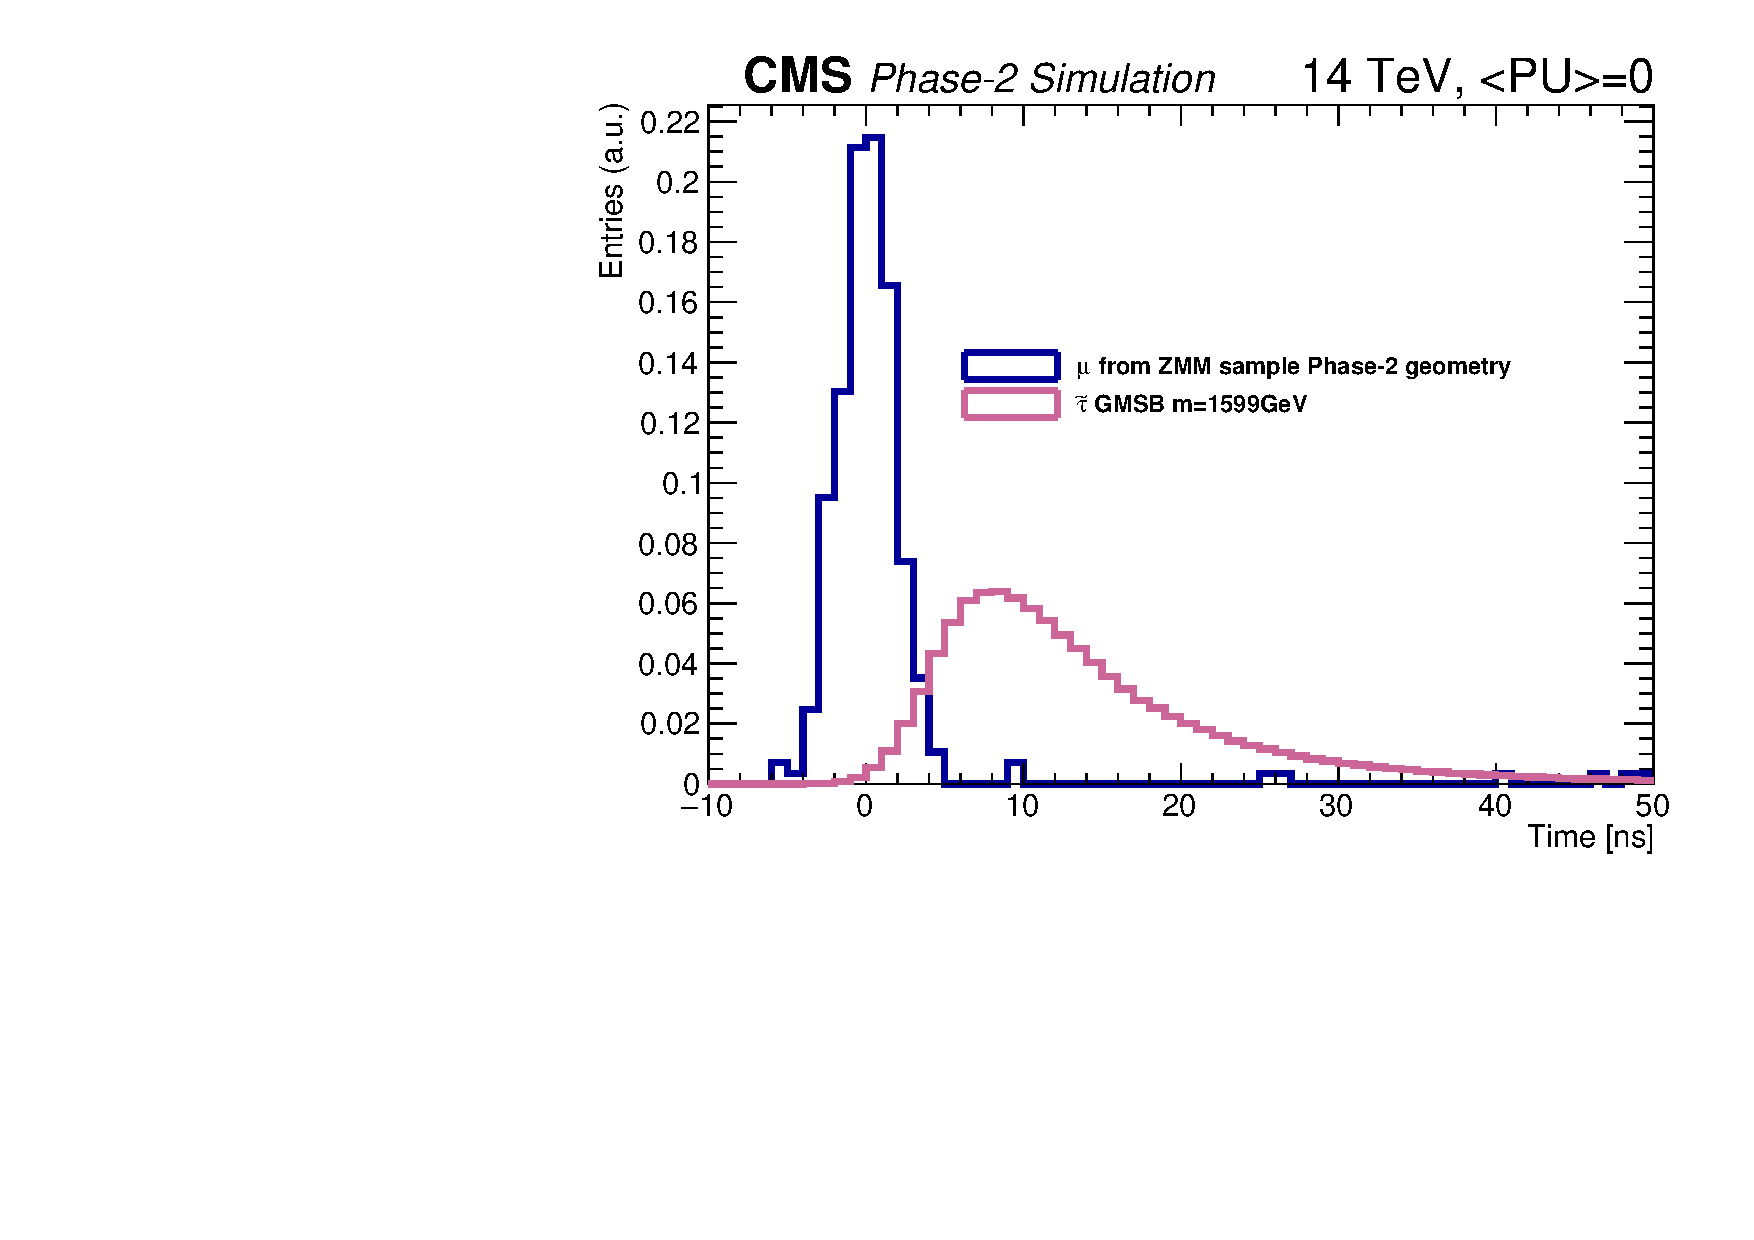
\includegraphics[width=0.9\textwidth]{figures/HSCP/time.pdf}
  \caption{RPC hit time measurement distribution in CMS for muons from $Z \to \mu\mu$ events and for semi-stable $\tilde \tau$ particles with m$\approx$1600~GeV, produced in $pp \to \tilde \tau \tilde \tau$ processes.}
  \label{fig:hscp_time}
\end{center}
\end{figure}

The principles of the proposed HSCP trigger algorithm are illustrated in Fig.~\ref{fig:HSCP_diagram}. In this figure, the vertical axis is the time of signals measured in RPC chambers, as synchronized so that muons moving nearly at the speed of light from a particular collision are measured at the time of the collision. The horizontal axis is the distance from the collision point to the position of the RPC at which the time is measured. The diagram shows three successive bunch crossings, two of which contain muons represented at horizontal lines. The diagram also shows the RPC time measurements from two HSCPs having slopes different from zero due to their traveling significantly slower than the speed of light. The time delay $\Delta t$ is related to the speed $v$ of an HSCP via the following equation:
%
\begin{equation}
\label{eq:HSCP_delay}
\Delta t = d\left(\frac{1}{v}-\frac{1}{c}\right).
\end{equation}
%
Here $d$ is the distance between the interaction point (IP) and the point where an HSCP crosses an RPC. For RE4/1 chambers and $\beta = v/c = 0.2$, the delay time is $>6$ bunch crossings, comparable to $150 \, \mathrm{ns}$.

\begin{figure}[t]
  \centering
  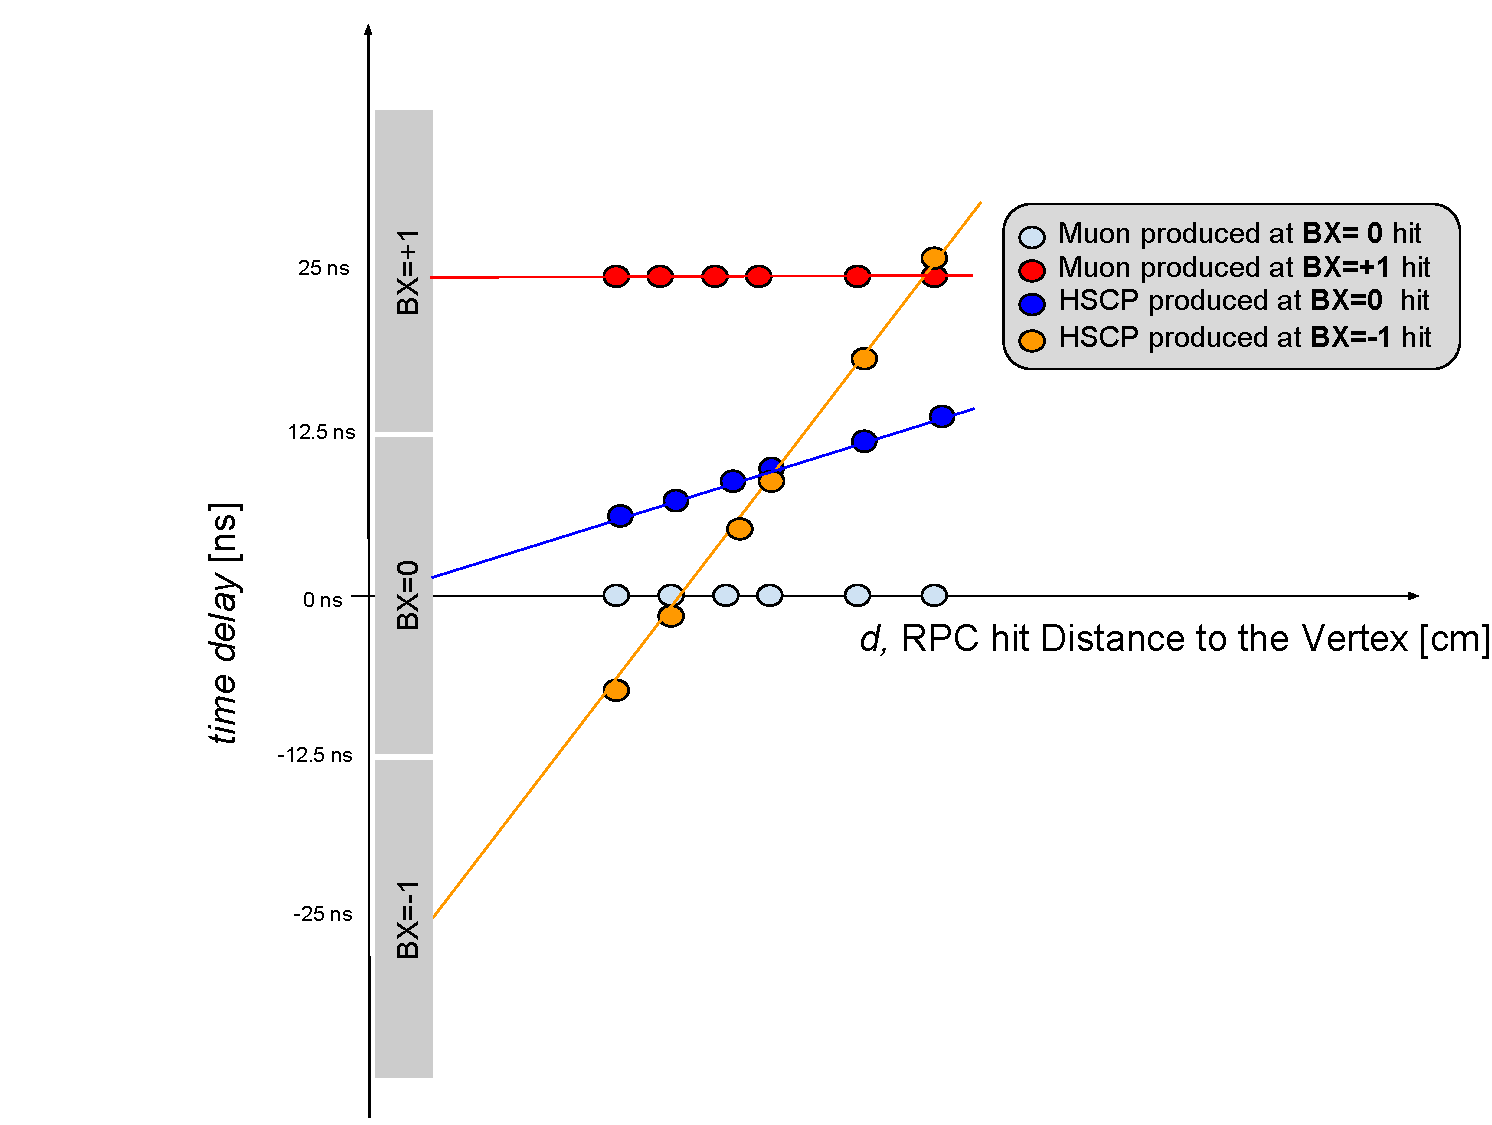
\includegraphics[width=0.9\textwidth]{figures/HSCP/diagram.pdf}
  \caption{Diagram showing times measured at different RPC stations for particles originating at different bunch crossings and with different velocities in CMS. The $x$-axis represents the distances from IP to RPC detectors, while the $y$-axis corresponds to time. The clock at each RPC station is tuned so that particles moving with the speed of light are registered with the exact same ``local'' times. Hence, relativistic particles are represented by horizontal lines on this diagram.}
  \label{fig:HSCP_diagram}
\end{figure}

A penetrating charged particle leaves a trail of hits in RPC chambers along its trajectory. The time of flight can be computed in each RPC station with respect to a number of bunch crossing hypotheses. Should there be a common velocity solution, derived from Eq.~(\ref{eq:HSCP_delay}), with $\beta < 0.6$, a trigger is formed. For $\beta >0.6$, the delays are small and can be handled by the Phase-1 trigger. The performance of this algorithm has been studied with the CMS full simulation. All the detector effects (e.g., electronics jitter, signal time propagation along strips) are considered. A particle-speed measurement resolution is shown in Fig.~\ref{fig:HCP_Trigger} (right) for the case of 25~ns signal sampling time (Phase-1) and 1.56~ns sampling time provided with the upgraded RPC Link Board System.

\begin{figure}[t]
\begin{center}
  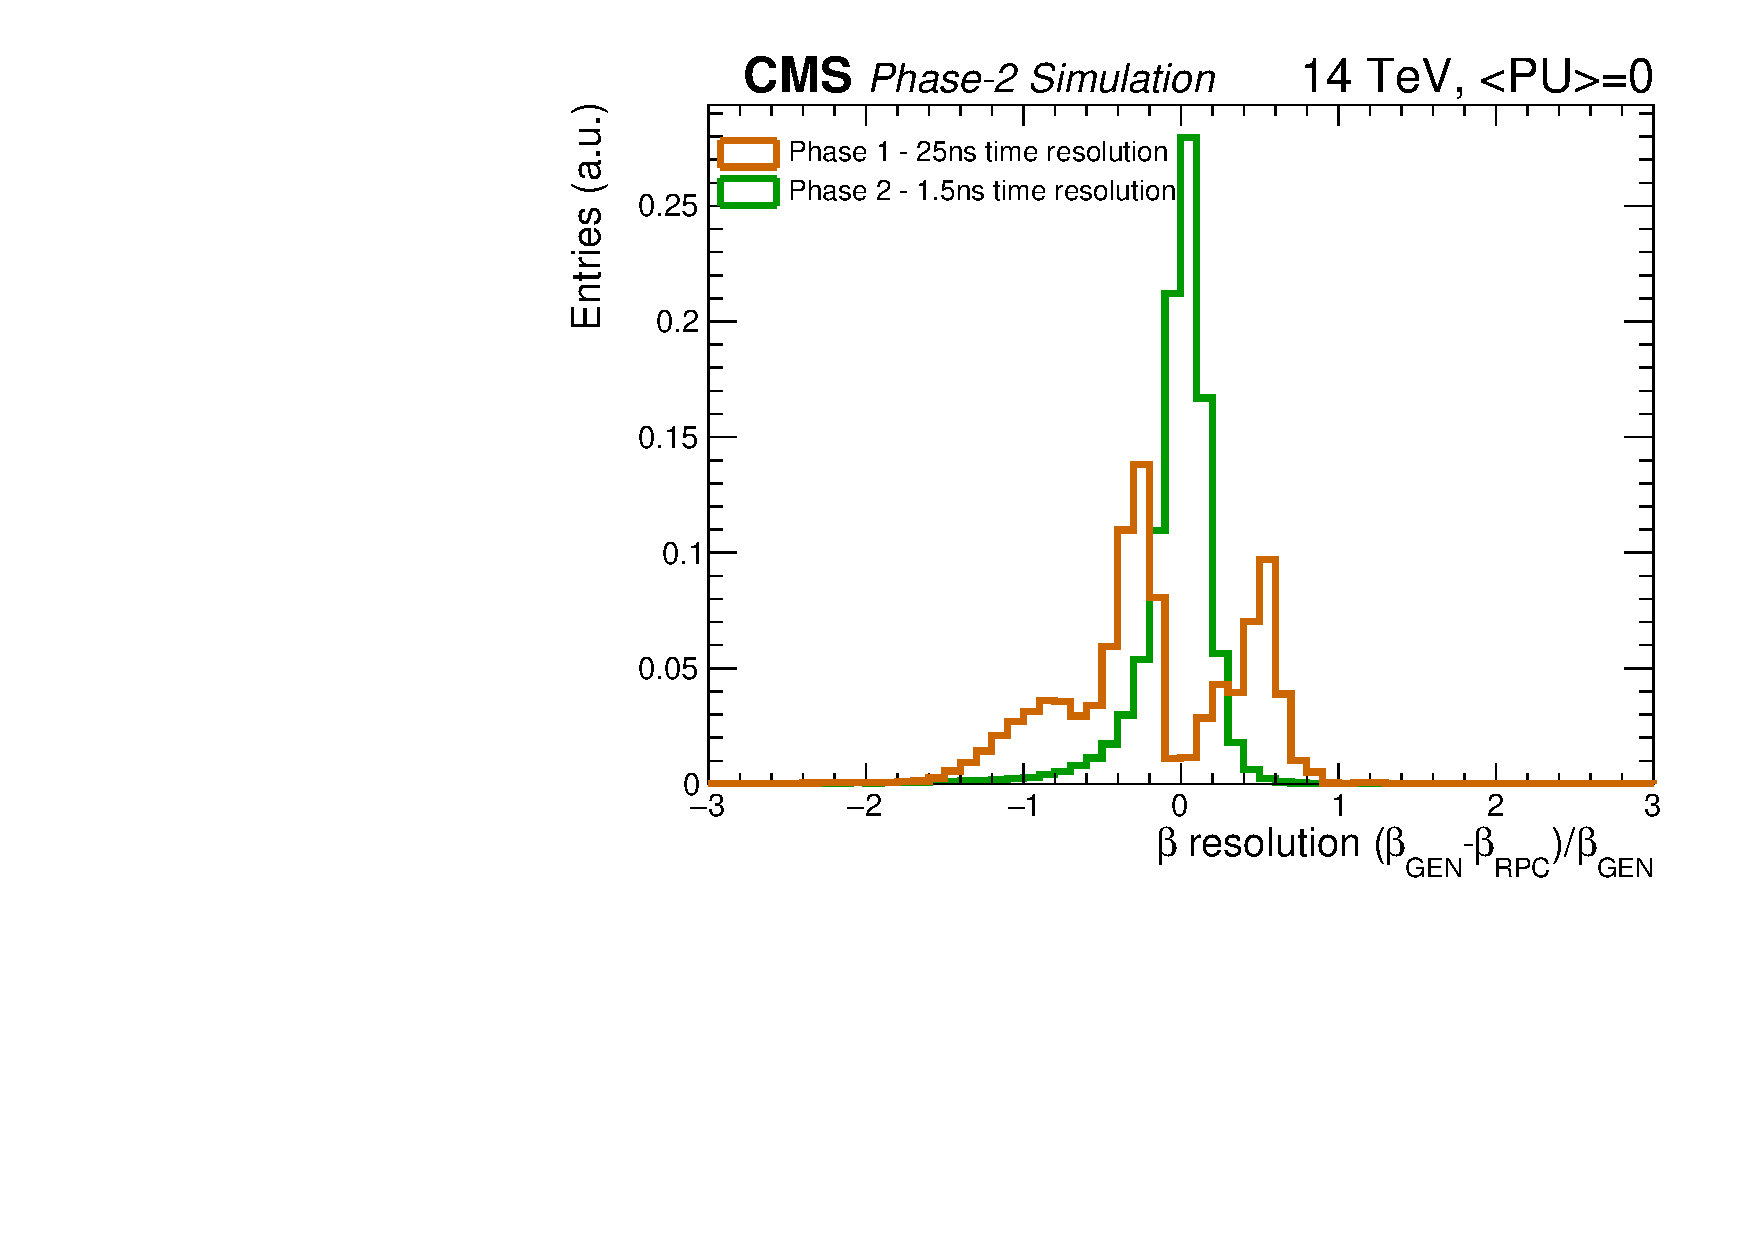
\includegraphics[width=0.47\textwidth]{figures/HSCP/beta_GenRes_2.pdf} \hfill
  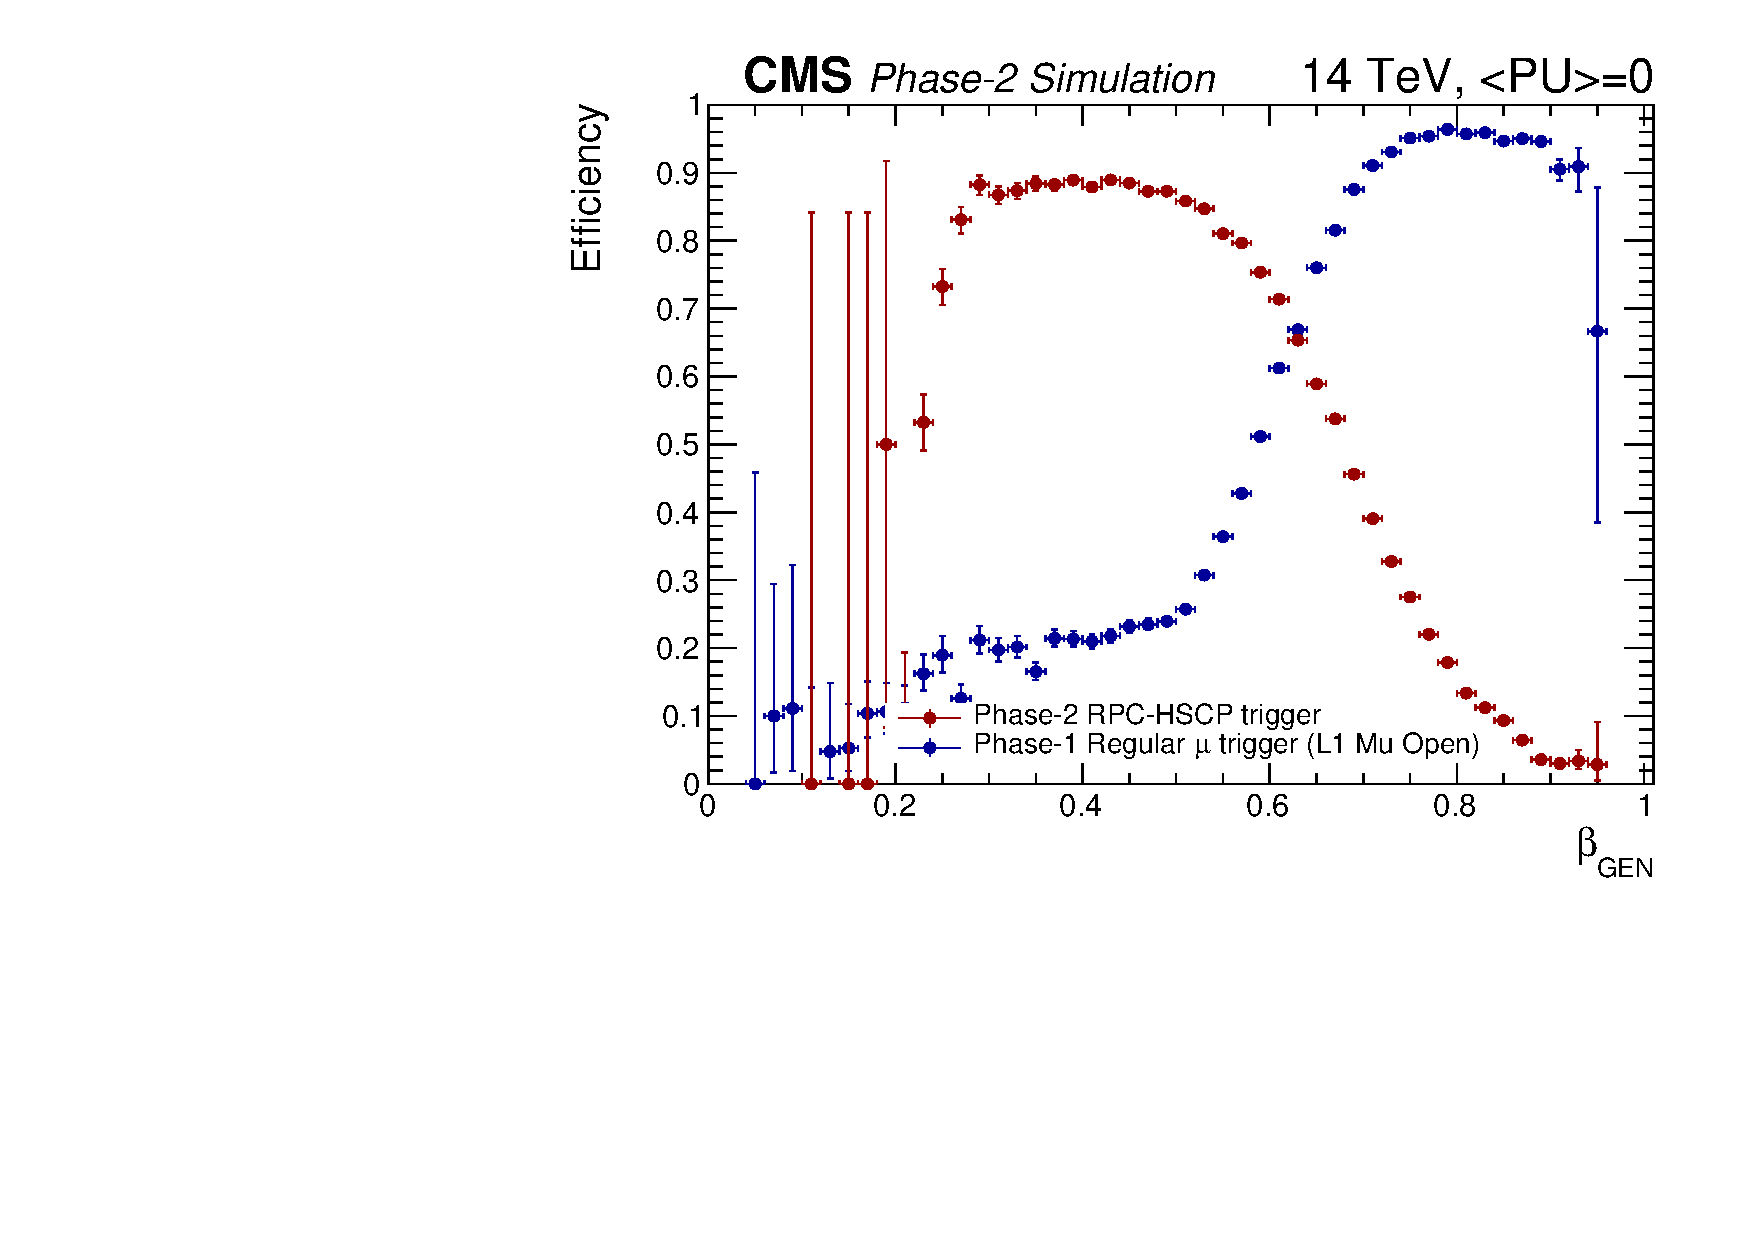
\includegraphics[width=0.47\textwidth]{figures/HSCP/trigEff-Mu-HSCPTriggers.pdf}
  \caption{Left:~Resolution of a particle-speed measurement at L1 trigger with Phase-1 and upgraded RPC Link Board System. Right:~The efficiency as a function of $\beta$ of the standard L1 muon trigger without any $p_T$ threshold, and the RPC-HSCP Phase-2 trigger with $1.56$~ns sampling time.}
  \label{fig:HCP_Trigger}
\end{center}
\end{figure}

The efficiency of the RPC-HSCP algorithm as a function of $\beta$ is studied and compared with the standard L1 muon trigger. The results are shown in Fig.~\ref{fig:HCP_Trigger} (right). The current CMS-HSCP Phase-1 trigger performs well down to $\beta \approx 0.75$. The upgraded RPC Link Board System will allow for the triggering, at the
correct bunch crossing, on possible HSCPs with velocities as low as $\beta \sim 0.25$.

Possible improvements for this trigger proposal in the $\beta$ measurement could be achieved by matching tracks in the track trigger to the HSCP muon trigger. The uncertainty coming from the propagation time along RPC strips can be reduced if the hit position is known along the local $y$ coordinate, or the global $\eta$. This correction is not needed for the RPCs thanks to the two-end strip readout for these new detectors.

\subsubsection{Displaced Muons in CMS}

%{\bf \textcolor{red}{[JB: Can this section be expanded and clarified?  For example, are we talking about single displaced muons here, or pairs of muons coming from a neutral LLP?  When a ``boosted muon'' is discussed here, what does that mean?  Typically boost is important when a parent particle is highly boosted since its decay products can be highly collimated, as in the case of low-mass dark photons, for example.  Here, is the point that the muon from, say, a smuon decay, has high-pT and thus its displaced track is very straight?  Or is there some other meaning?]}}
%{\bf \textcolor{red}{[JA: I've explained the model used, and removed the bit about boosted muons, since it's not actually that relevant. Sorry,
%we were drawing from section of the muon TDR that wasn't particularly well-worded. Hopefully now it's better. Should be checked.]}}

%Tracks from displaced muons that could result from BSM LLP decays have different properties depending upon particle boost. In the case of a sufficiently boosted muon, the corresponding track roughly points back to the primary interaction, leading to a transverse impact parameter which is smaller than that from typical muons from promptly decaying particles or background processes, but the decay may still occur at the outer edge of the tracker or even well outside the tracker volume. If the muon is not highly boosted, the corresponding track does not point back to the primary interaction vertex and we might even get a large impact parameter for a decay not far away from the primary interaction.

Many BSM theories predict particle decays with displaced muon or muon pairs in its final state, such as dark SUSY and GMSB with smuons.
In order to demonstrate the physics potential of displaced muons at the HL-LHC with the CMS detector,
a particular SUSY model is selected where the displaced signature consists of a dimuon final state emerging from the decay of heavy sparticles (smuons).
Searches for the direct production of heavy sparticles with long lifetimes are difficult in the present LHC runs,
owing to small cross sections and limited integrated luminosity, and will only become possible at the HL-LHC.
In gauge-mediated SUSY breaking models, smuons can be (co-)NLSPs (next to lightest supersymmetric particles) and decay to a muon and a gravitino~\cite{Ruderman:2010kj}.
This decay can either be prompt or the slepton can have a significant lifetime: the final state signature is then given
by two displaced oppositely charged muons and significant missing transverse energy.
The smuon pair production has the advantage that it can be characterized by a very clean final state topology, and
we will therefore focus on the process $q \bar q \to \widetilde{\mu} \widetilde{\mu}$, where the two smuons decay far from the primary interaction vertex.
For this process, the muon $|d_0|$ can reach up to approximately one meter (or longer) for sufficiently large lifetimes,
as shown in Fig.~\ref{fig:perfDisplaced} (left). Figure~\ref{fig:perfDisplaced} (right)
compares the number of hits created by these displaced muons in the CMS muon system in Phase-2 and the current CMS detector.
The hits plotted here are those associated with the displaced stand-alone muon tracks, which is a muon track reconstruction
algorithm specifically designed for displaced muons that can only be reconstructed in the muon system~\cite{CMS-DP-2015-015}.


\begin{figure}[t]\begin{center}
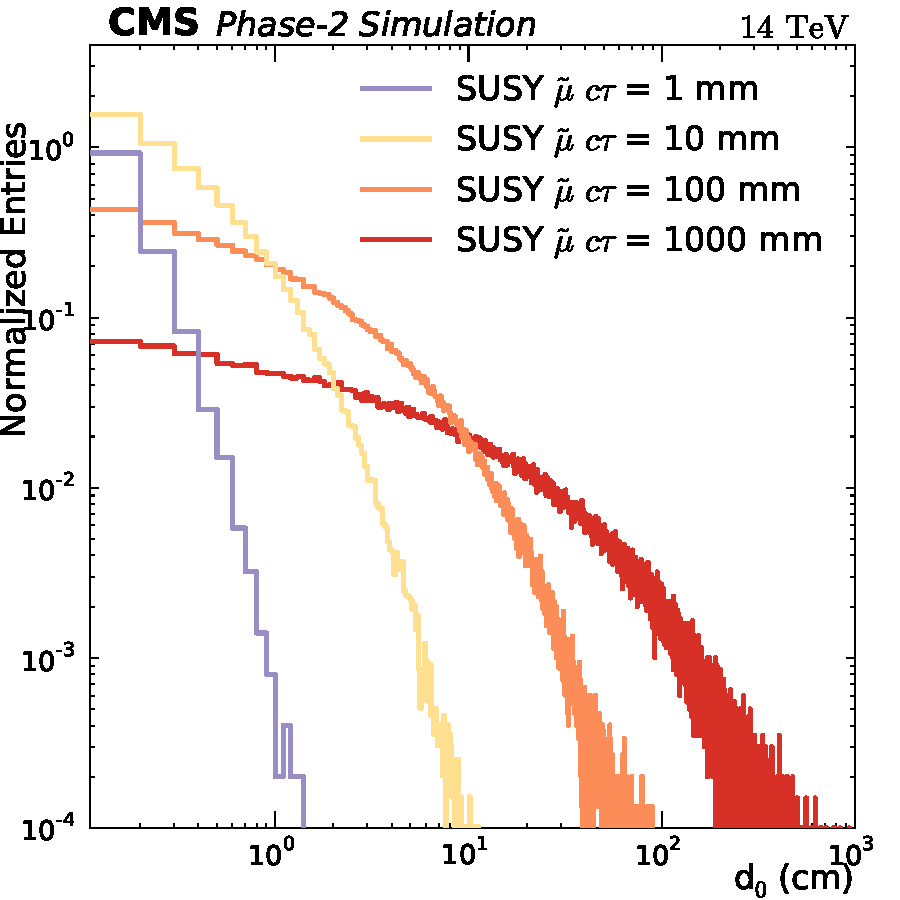
\includegraphics[width=0.47\textwidth]{figures/Stage0h1_0_d0_smuon_daughter}
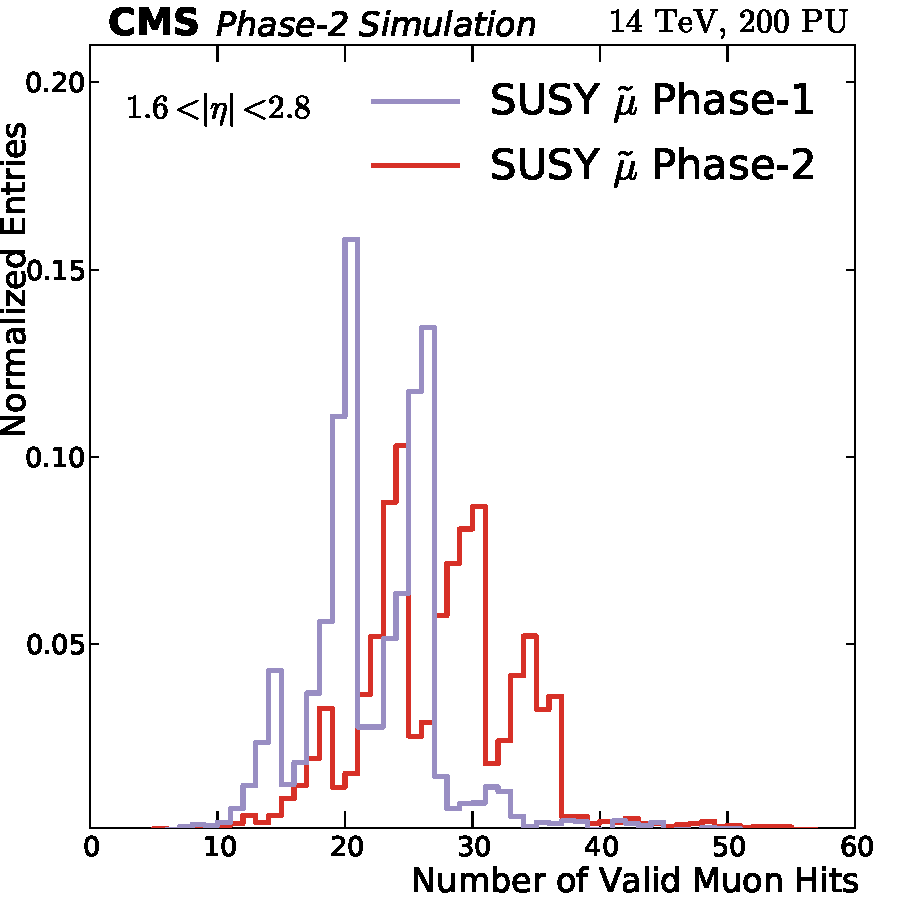
\includegraphics[width=0.47\textwidth]{figures/MuonHitsEndcap}
\caption{
Left: The muon transverse impact parameter, $|d_{0}|$, for several simulated smuon decay lengths, $c\tau$, at the generator level.
Right: Distribution of the minimum number of valid hits in the CMS Phase-2 muon system for a SUSY $\widetilde{\mu}$ with $m_{\widetilde{\mu}}$ = 500~GeV and $\tau$ = 1000~mm for the Run 2 (blue) and Phase-2 (red) detectors.
}
\label{fig:perfDisplaced}
\end{center}
\end{figure}

Standard triggers and reconstruction algorithms that use the position of the primary vertex will not efficiently reconstruct tracks with large impact parameters. Consequently, triggering on and reconstructing muons produced far  from the IP is challenging and requires dedicated triggers and reconstruction algorithms. The upgrades to the muon system in CMS, as well as the L1 tracking capabilities, significantly improve the experiment's ability to search for displaced muons at the HL-LHC.

\paragraph{Triggering on Displaced Muons}

The momentum resolution of the L1 muon trigger for muons coming from the primary vertex will be greatly improved by adding information from the L1 track trigger, discussed previously. The L1 track trigger can also be directly combined with trigger primitives at the first stage of the muon track-finder electronics; this would mirror the offline reconstruction of ``Tracker Muons'' which improve the efficiency for very low-$p_T$ muons, especially in the barrel region.

To trigger on both prompt and non-prompt muons effectively at L1, a standalone L1 muon generates two $p_T$ measurements for each muon, prompt and non-prompt, which are matched with L1 tracks. If the track match is successful, the L1 track trigger $p_T$ is used and a prompt candidate is formed. If the match is unsuccessful and the muon is not vetoed by L1 tracks, the non-prompt L1 muon $p_T$ is used to form a displaced muon candidate. Figure~\ref{fig:cmsL1mu} shows good performance for displaced muons with this method, i.e., there is a reasonably high efficiency and a trigger rate for a single muon trigger of around 10~kHz under HL-LHC conditions. Further improvements to the algorithm are underway to accommodate high pile-up conditions. The upgrade of the RPC system will allow slowly-moving particles to pass the trigger and be identified by measuring their time of flight to each RPC station with a resolution of $\mathcal{O}(1)$~ns. The speed of muon-like particles and the time (bunch crossing) of their
origin will be computed with a fast algorithm to be implemented in the L1 trigger for the HL-LHC.

\begin{figure}[t]
\begin{center}
  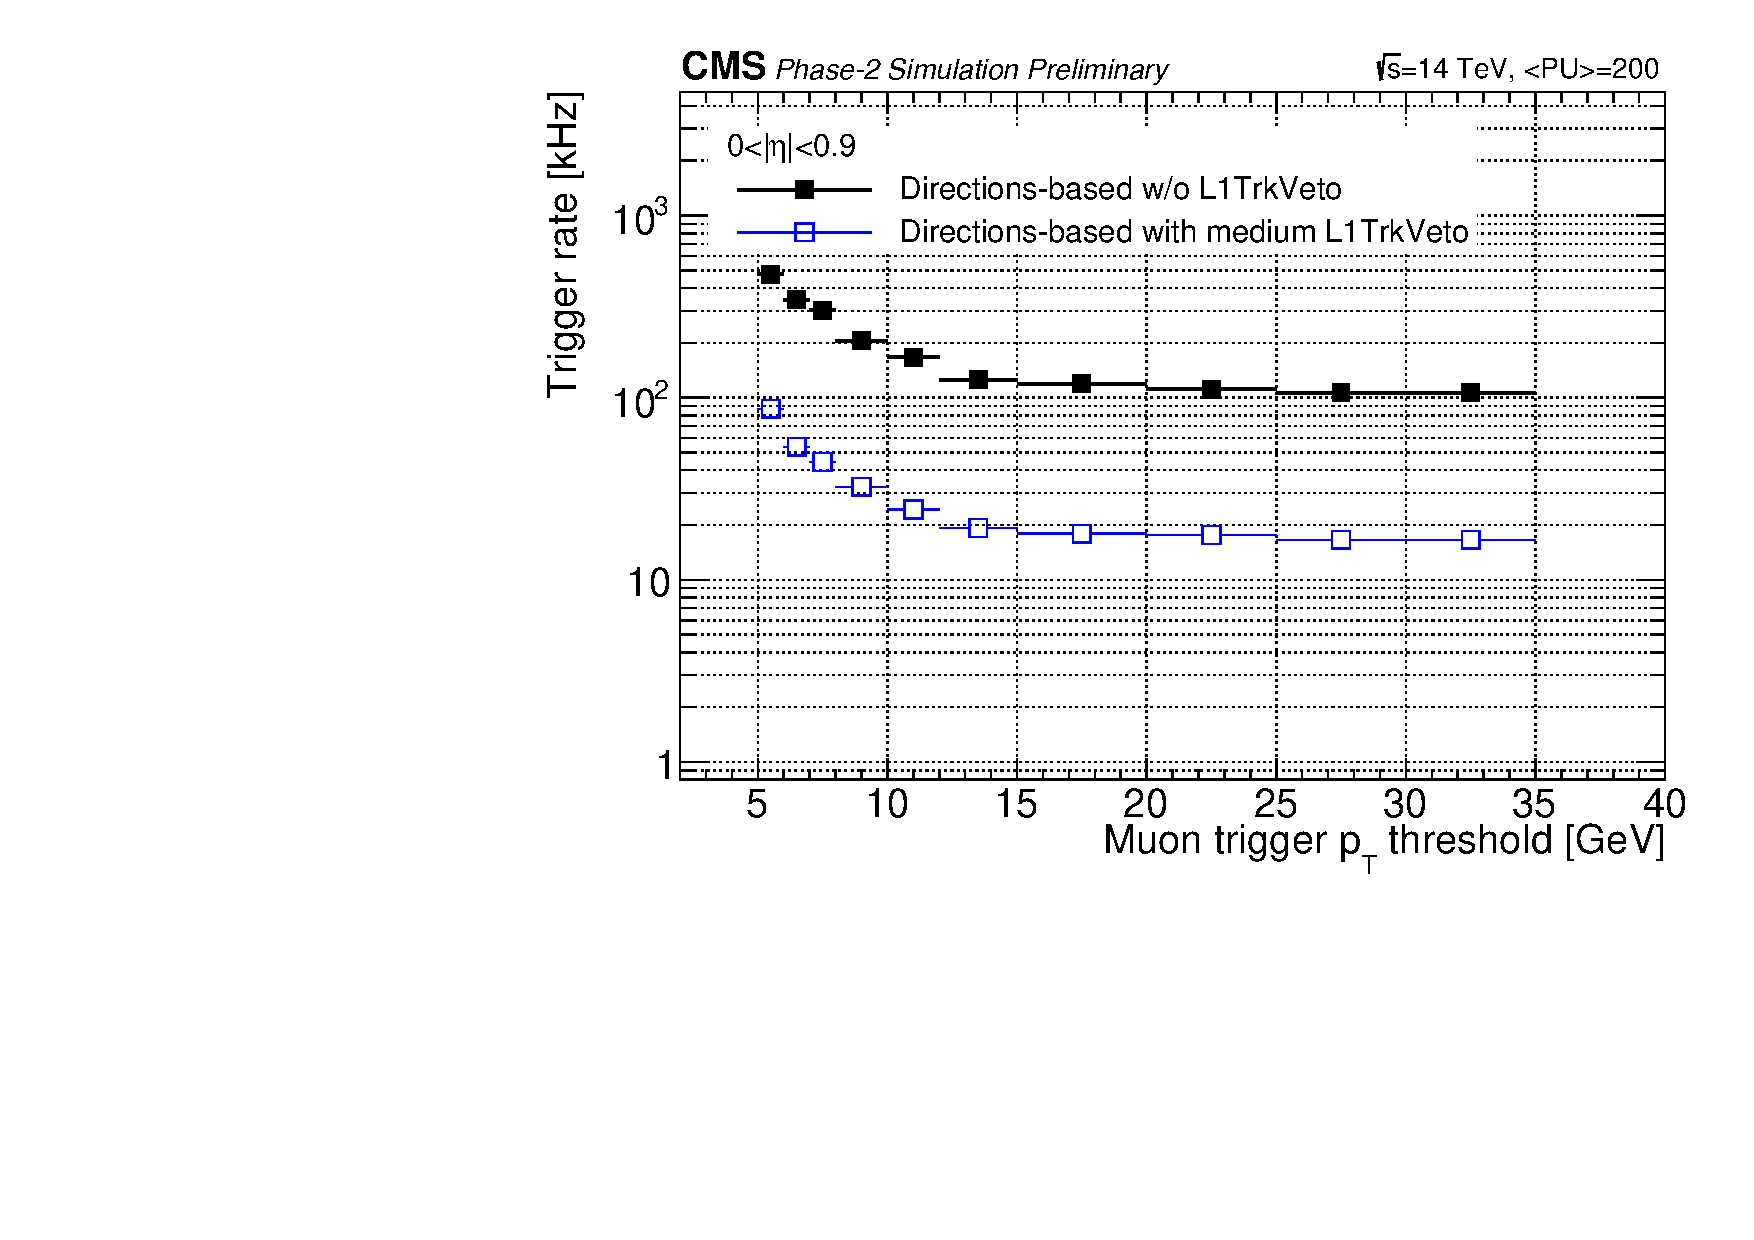
\includegraphics[width=0.47\textwidth]{figures/cmsupgrade/TDR-17-003_fig_7_11_a_Prompt_L1Mu_trigger_rate_pt__L1Mu__L1Mu2st__DisplacedL1MuDirectionBased_MB1_MB2_MB3_MB4_combined_eta0to0p9.pdf} \hfill
  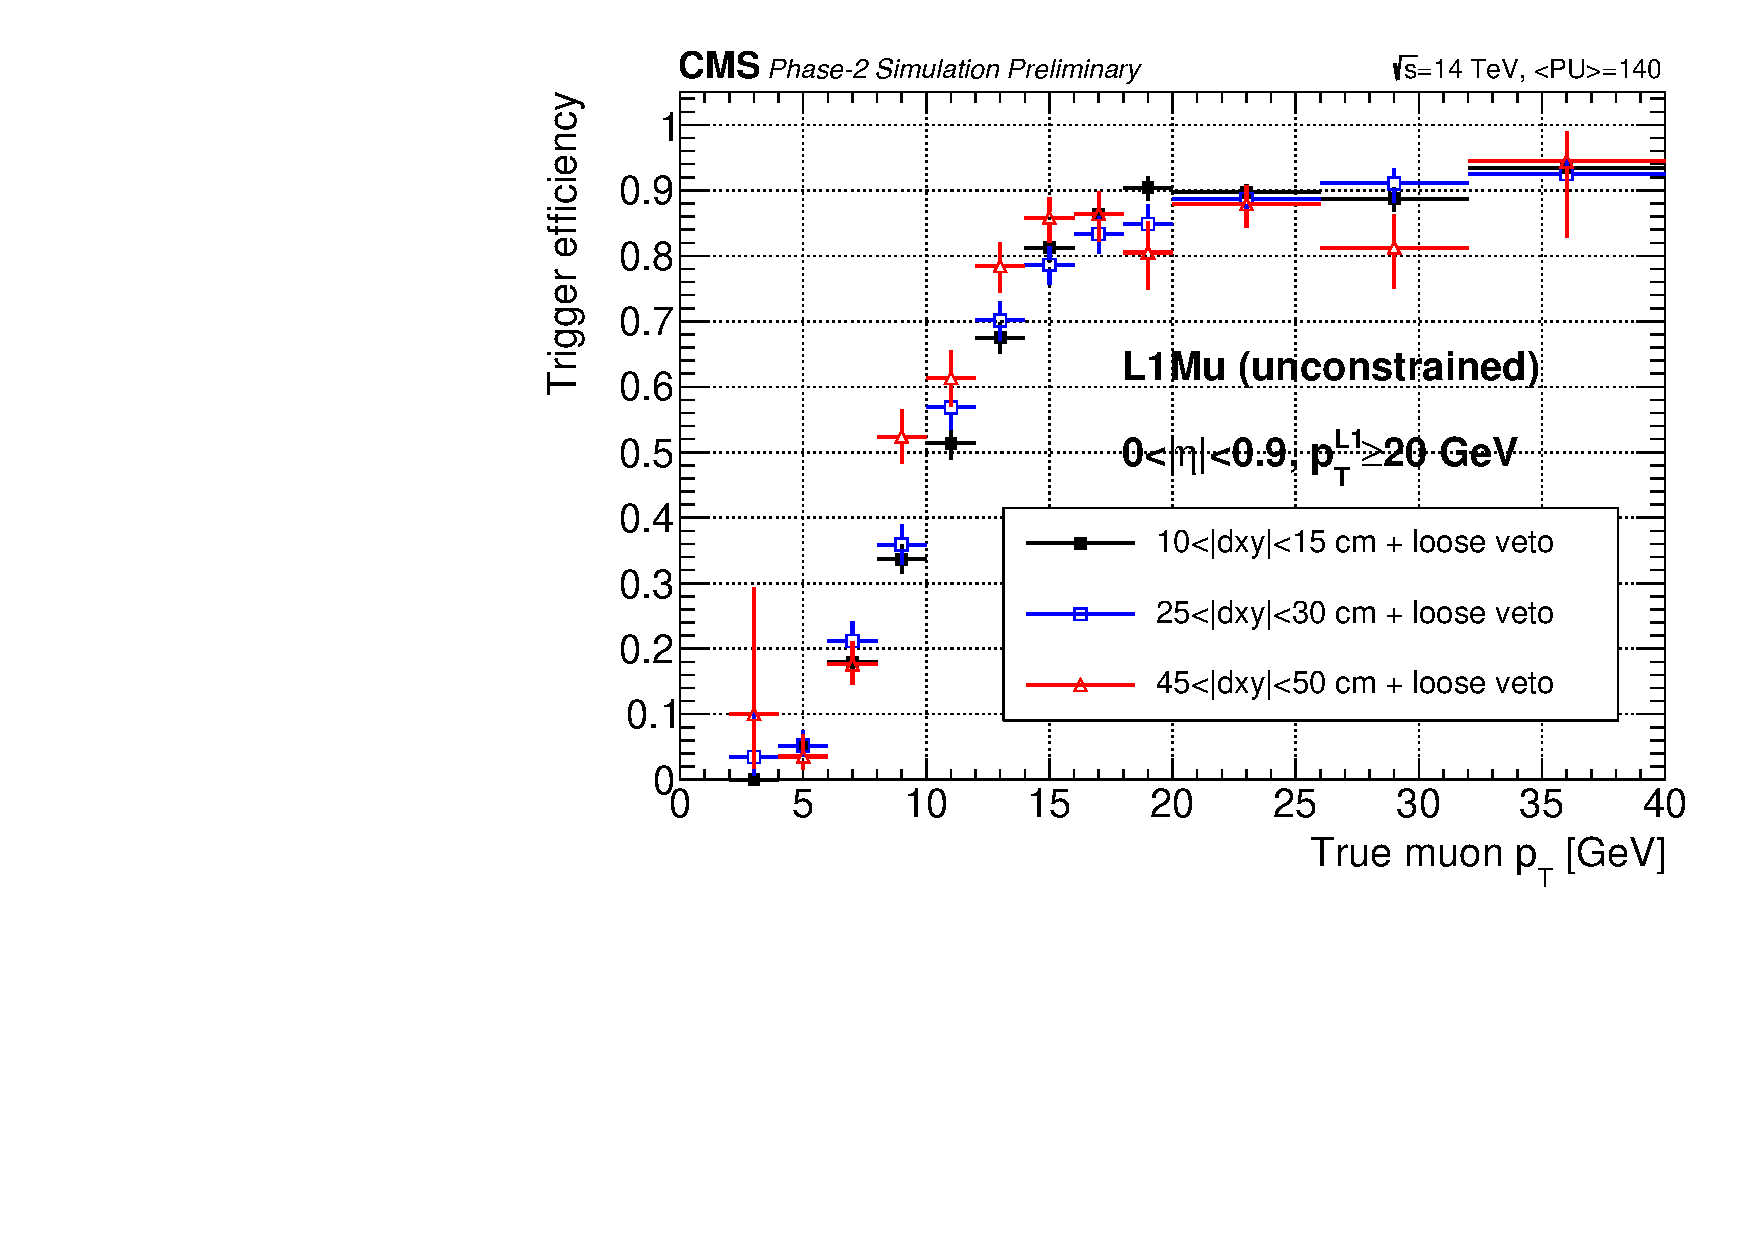
\includegraphics[width=0.47\textwidth]{figures/cmsupgrade/TDR-17-003_fig_7_11_b_L1MuonTDR2017Displaced_L1MuPt20_SimMuPt_DT1_DT2_DT3_DT4_combined_eta0to0p9_dxy5to50_looseVeto.pdf}
  \caption{L1 Muon trigger rate (left) and efficiency (right) %{\bf \textcolor{red}{[JB: Trigger efficiency of what?  Defined how?]}}
versus muon $p_T$ threshold for the barrel displaced muon algorithm.}
  \label{fig:cmsL1mu}
\end{center}
\end{figure}


\paragraph{Reconstruction}

A dedicated muon reconstruction algorithm was designed for non-prompt muons that leave hits only in the muon system. This displaced stand-alone (DSA) algorithm is seeded by groups of track segments in the muon chambers. For each seed, a muon track is reconstructed with the same Kalman-filter technique as for the standard stand-alone (SA) muon reconstruction algorithm, but without constraining the interaction point. Figure~\ref{fig:perfDisplaced} (right) shows the distribution of the number of hits in the Run 2 and HL-LHC detectors for displaced muons. The impact of the new stations is clearly visible. The charge mis-identification probability is expected to further decrease with the additional hits.

\paragraph{Sensitivity Projection with a GMSB Model}

To study the impact on physics sensitivity, a particular gauge-mediated SUSY breaking (GMSB) model is selected where the displaced signature consists of a dimuon final state plus gravitinos, emerging from the decay of heavy long-lived sparticles (smuons), where the gravitinos escape detection. This maps to the direct pair production simplified model with neutral LLP decays to muon + invisible in Sec.~\ref{sec:proposal}. This signal can serve as a proxy for other models with two LLPs decaying into muons. The final-state signature is then given by two displaced, oppositely-charged muons and significant \met. Example long-lived particles with $c\tau=10, 100, 1000$~mm\,and several mass hypotheses (0.2, 0.5, 1~TeV) are simulated.

The main background for this search comes from multi-jet production (QCD), \ttbar~production, and Z/DY $\to\ell\ell$ events where large impact parameters are (mis)reconstructed. Cosmic-ray muons have been studied in Run 2 and are independent of the instantaneous luminosity. %{\bf \textcolor{red}{[JB: Isn't this trivially true?]}}
In the barrel, they are efficiently rejected by the timing of the hits in the upper leg. Cosmic-ray muons do not originate at the vertex and therefore pass the upper-barrel sectors in reverse direction from outside in. The fraction of cosmic-ray muons in the endcaps is negligible.

Given the very low cross section of the signal process, it is essential to reduce the background efficiently. The best background discriminator is the impact parameter significance $d_0 / \sigma (d_0) \geq 5$. Given the signal kinematics, the muons from a signal process are expected to move in roughly opposite directions and \met can be expected to be larger than $50$~GeV. After this selection the signal efficiency is about 4--5\% for $c\tau \approx 1000$~mm, nearly independent of the smuon mass, and $10^{-5}$ -- $10^{-4}$ for QCD, \ttbar, and DY backgrounds.

In Figure~\ref{fig:displResults}, the expected exclusion limits are shown for the GMSB model in which the smuon is a (co-)next-to-lightest supersymmetric particle (NLSP, where ``LSP'' indicates the lightest supersymmetric particle), for the predicted cross section as well as for a factor 100 larger cross section. The exclusion limits are shown as functions of smuon mass in Figure~\ref{fig:displResults} (left) and decay length in Figure~\ref{fig:displResults} (right).

\begin{figure}[t]\begin{center}
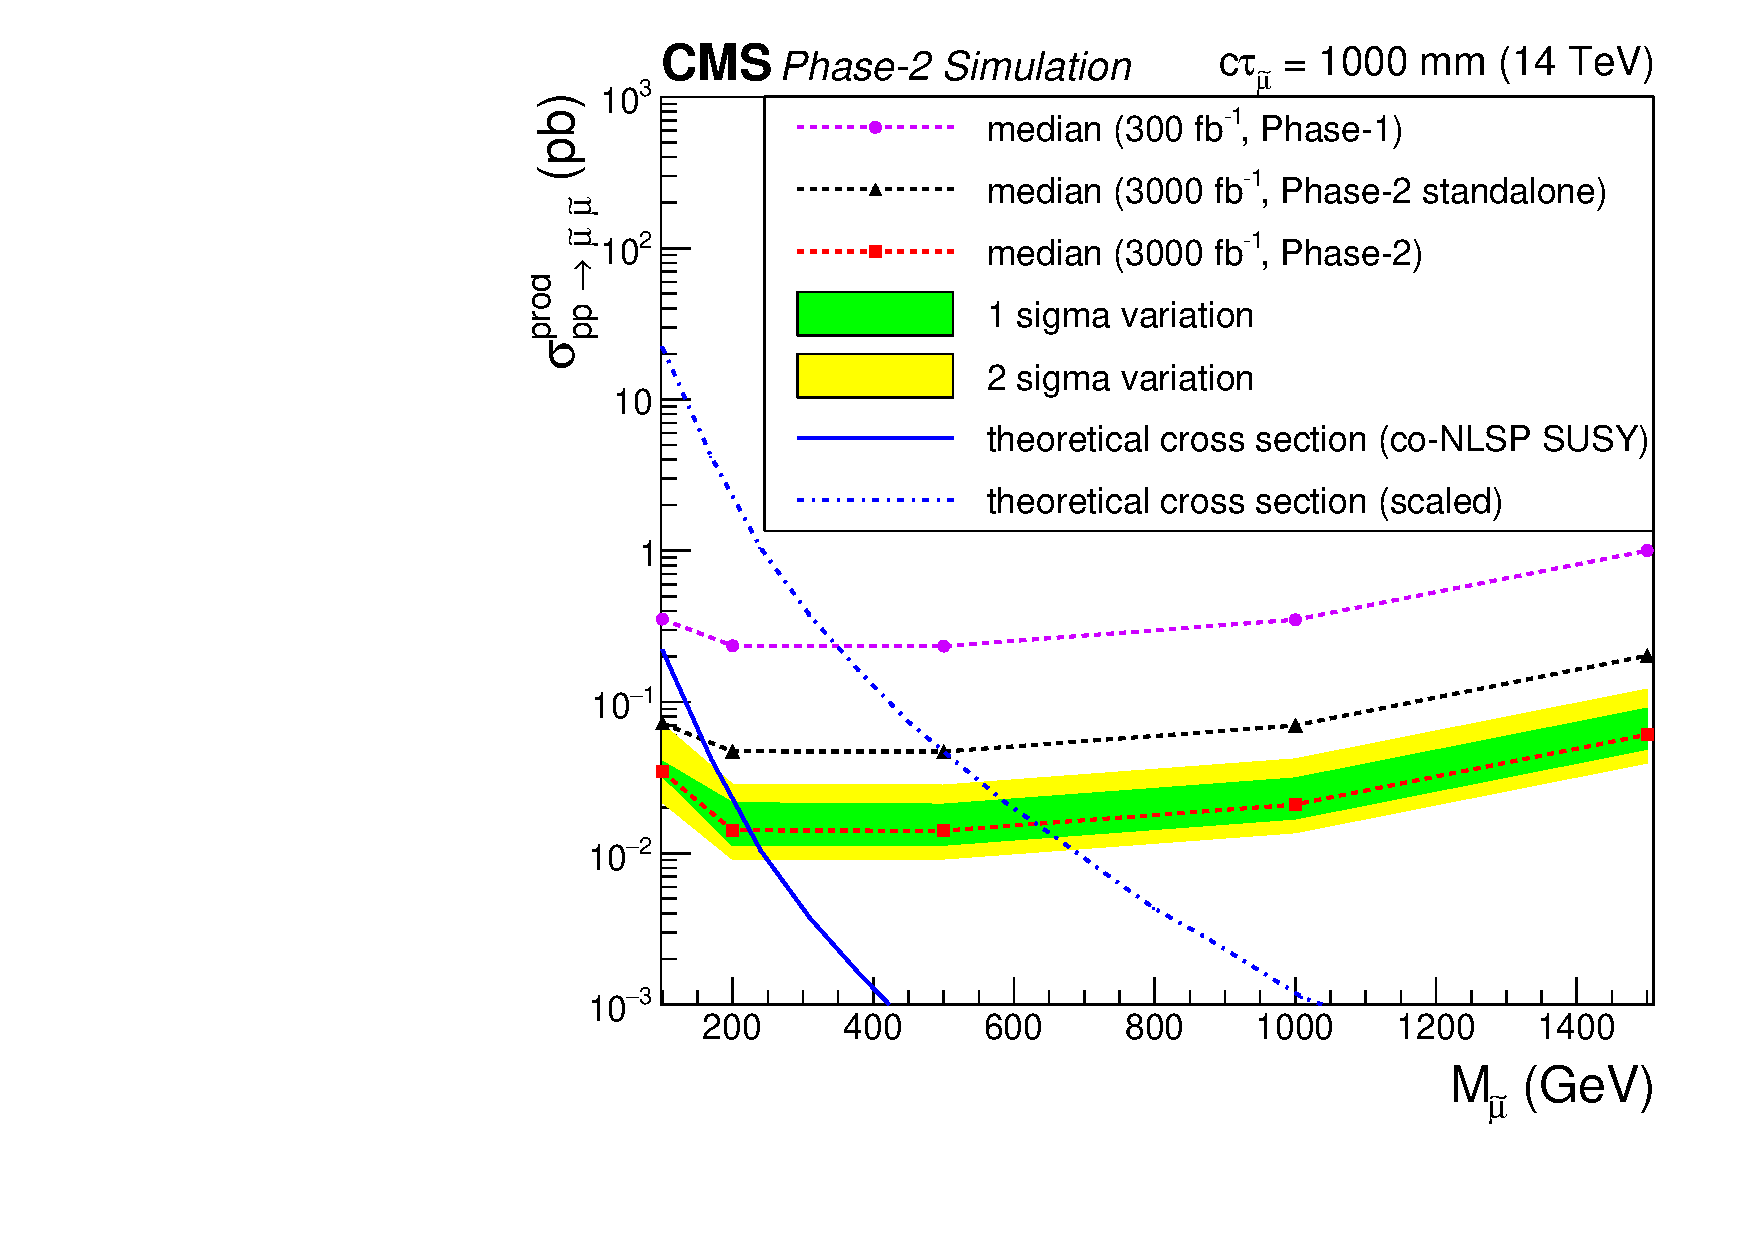
\includegraphics[width=0.47\textwidth]{figures/LimitComparison_withStandAloneEff.pdf}
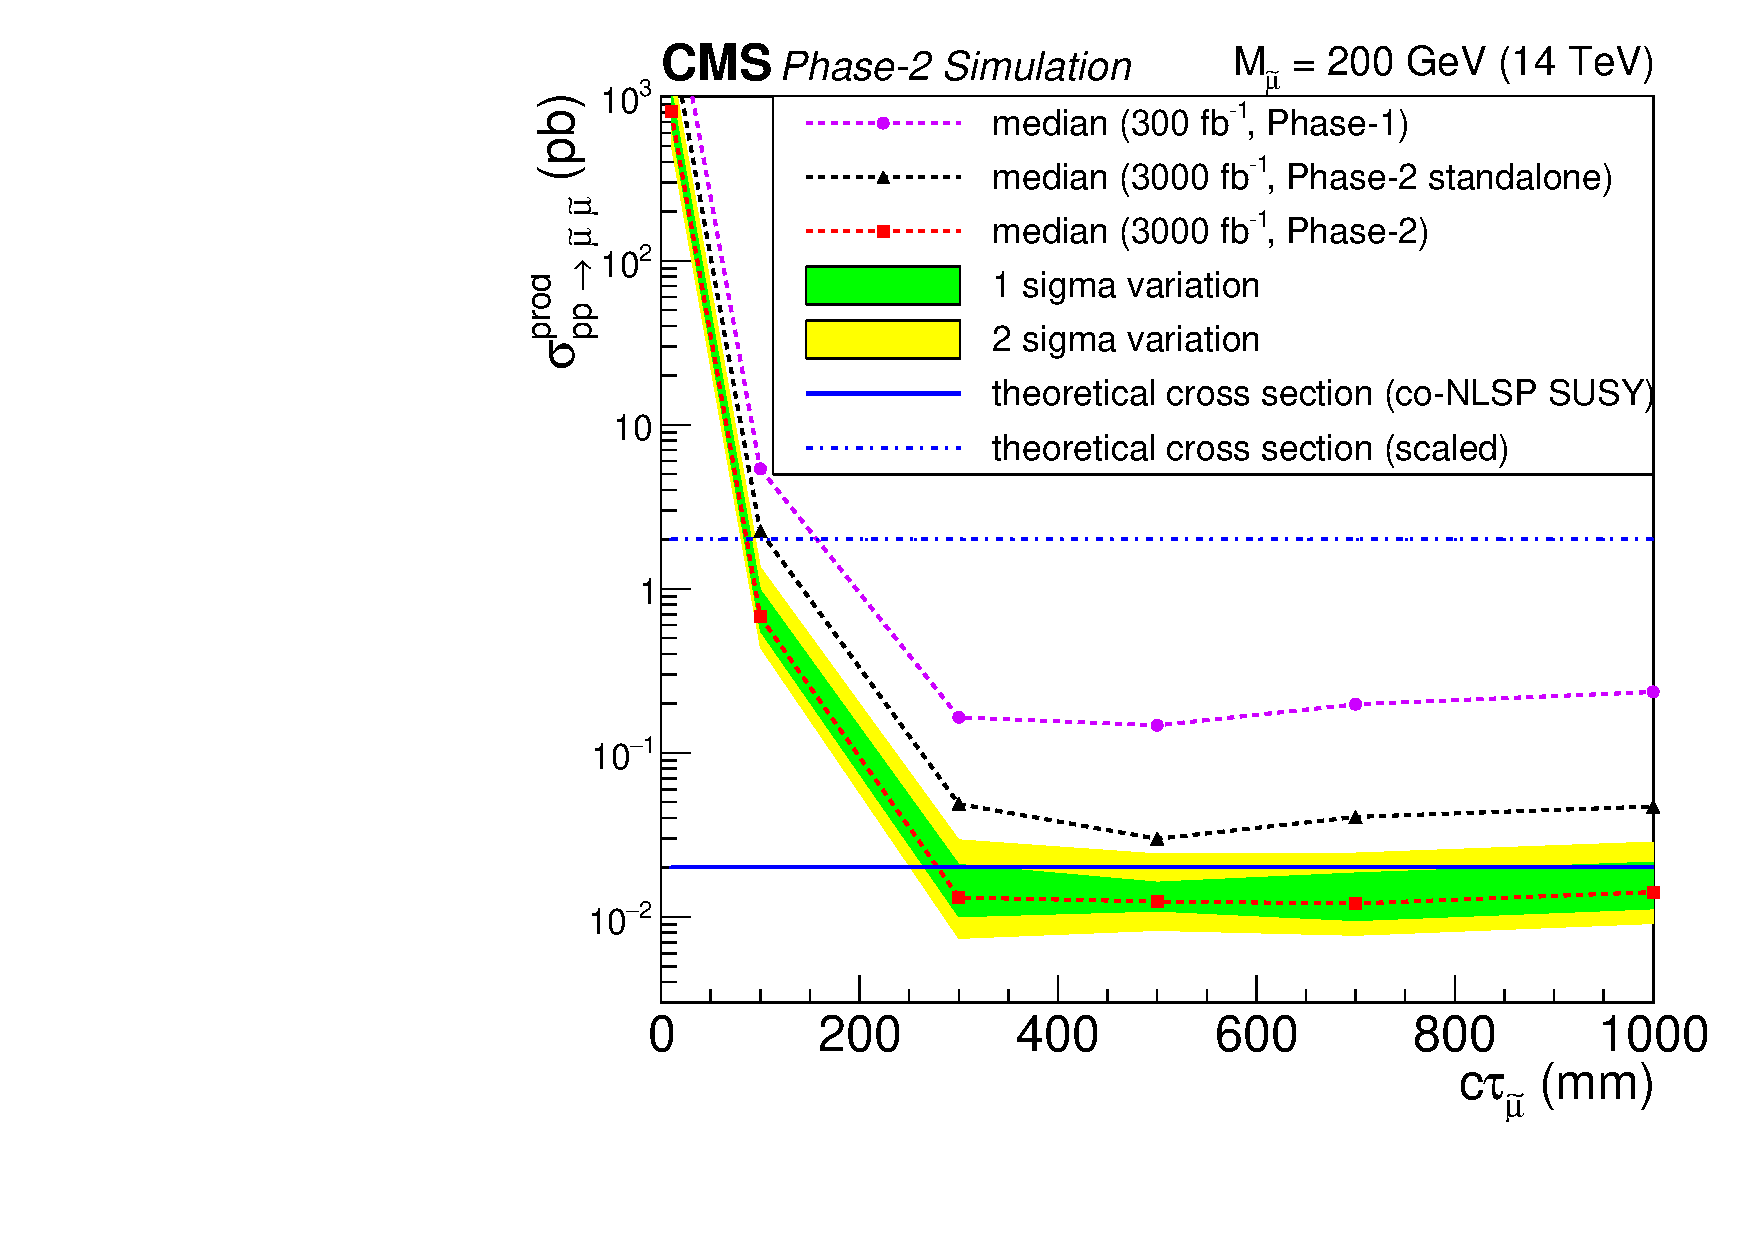
\includegraphics[width=0.47\textwidth]{figures/LimitComparison_asfuncofCtau.pdf}
\caption{The 95\% CL projected upper limits at CMS for $q \bar q \to \widetilde{\mu} \widetilde{\mu}, \widetilde{\mu}\rightarrow \mu\widetilde{G}$ for various mass hypotheses for $c\tau$ = 1~m (left), and as a function of the decay length for $m_{\widetilde{\mu}}$ = 200~GeV (right). In both panels, the theoretical cross section for the specific model is represented by the blue solid line. For different SUSY breaking scales, tan~$\beta$ or otherwise modified parameters, the cross sections may be 100 times larger, reflected by the blue dash-dotted line. Green (yellow) shaded bands show the one (two) sigma range of variation of the expected 95\% CL limits. Phase-2 results with an average of 200 pile-up collisions per bunch crossing and an integrated luminosity of $300$\fbinv are compared to results obtained with $300$\fbinv. The black line shows the sensitivity without the DSA algorithm, which reduces the reconstruction efficiency by a factor three.
%%% Drop discovery significance?
%c) Discovery sensitivity for various mass hypotheses. WORKING ON IT.
 }
\label{fig:displResults}
\end{center}
\end{figure}

The sensitivity depends on $c\tau$ because shorter decay lengths shift the signal closer to background. In Figure~\ref{fig:displResults} (right), the resulting physics sensitivities in terms of production cross section for the HL-LHC, normalized to $3000$\fbinv, are shown for the dedicated reconstruction of displaced muons and for the standard reconstruction. Also shown is the expected sensitivity at the end of Phase-1. Systematic uncertainties for the Phase-1 scenario are taken from current Run 2 analyses and adapted for expected HL-LHC conditions based on the assumptions of reduced systematics described in Ref.~\cite{FTR-16-005}. Clearly, only the HL-LHC will allow this process to be studied. The expected exclusion limit is around 200~GeV for $c\tau = 1000$~mm with 3000\fbinv. This also illustrates the importance of keeping lepton trigger thresholds at several tens of GeV, even in the environment of 200 pile-up interactions per bunch crossing.

In order to evaluate the discovery sensitivity of a search for the GMSB model the same input is used as in the limit calculation, now with the assumption that one would have such a signal in the data. The discovery sensitivity is shown as a function of smuon mass in Figure~\ref{fig:displResultsSensitiviy} (left) and decay length in Figure~\ref{fig:displResultsSensitiviy} (right). The dependence of the discovery sensitivity on signal parameters is similar to the limit calculation. Similarly to the limit calculation, the sensitivities are also shown for the end of the HL-LHC, normalized to 3000\fbinv, for the dedicated reconstruction of displaced muons and for the standard reconstruction. For comparison, the expected sensitivity at the end of Phase-1 is also shown. One can conclude that only the HL-LHC is sensitive to the discovery of a long-lived particle such as the smuon with a mass higher than $200$~GeV. Another prominent difference is seen in the discovery sensitivity for standard standalone reconstruction and dedicated displaced standalone reconstruction up to 1~$\sigma$ and 4~$\sigma$, respectively.

\begin{figure}[t]\begin{center}
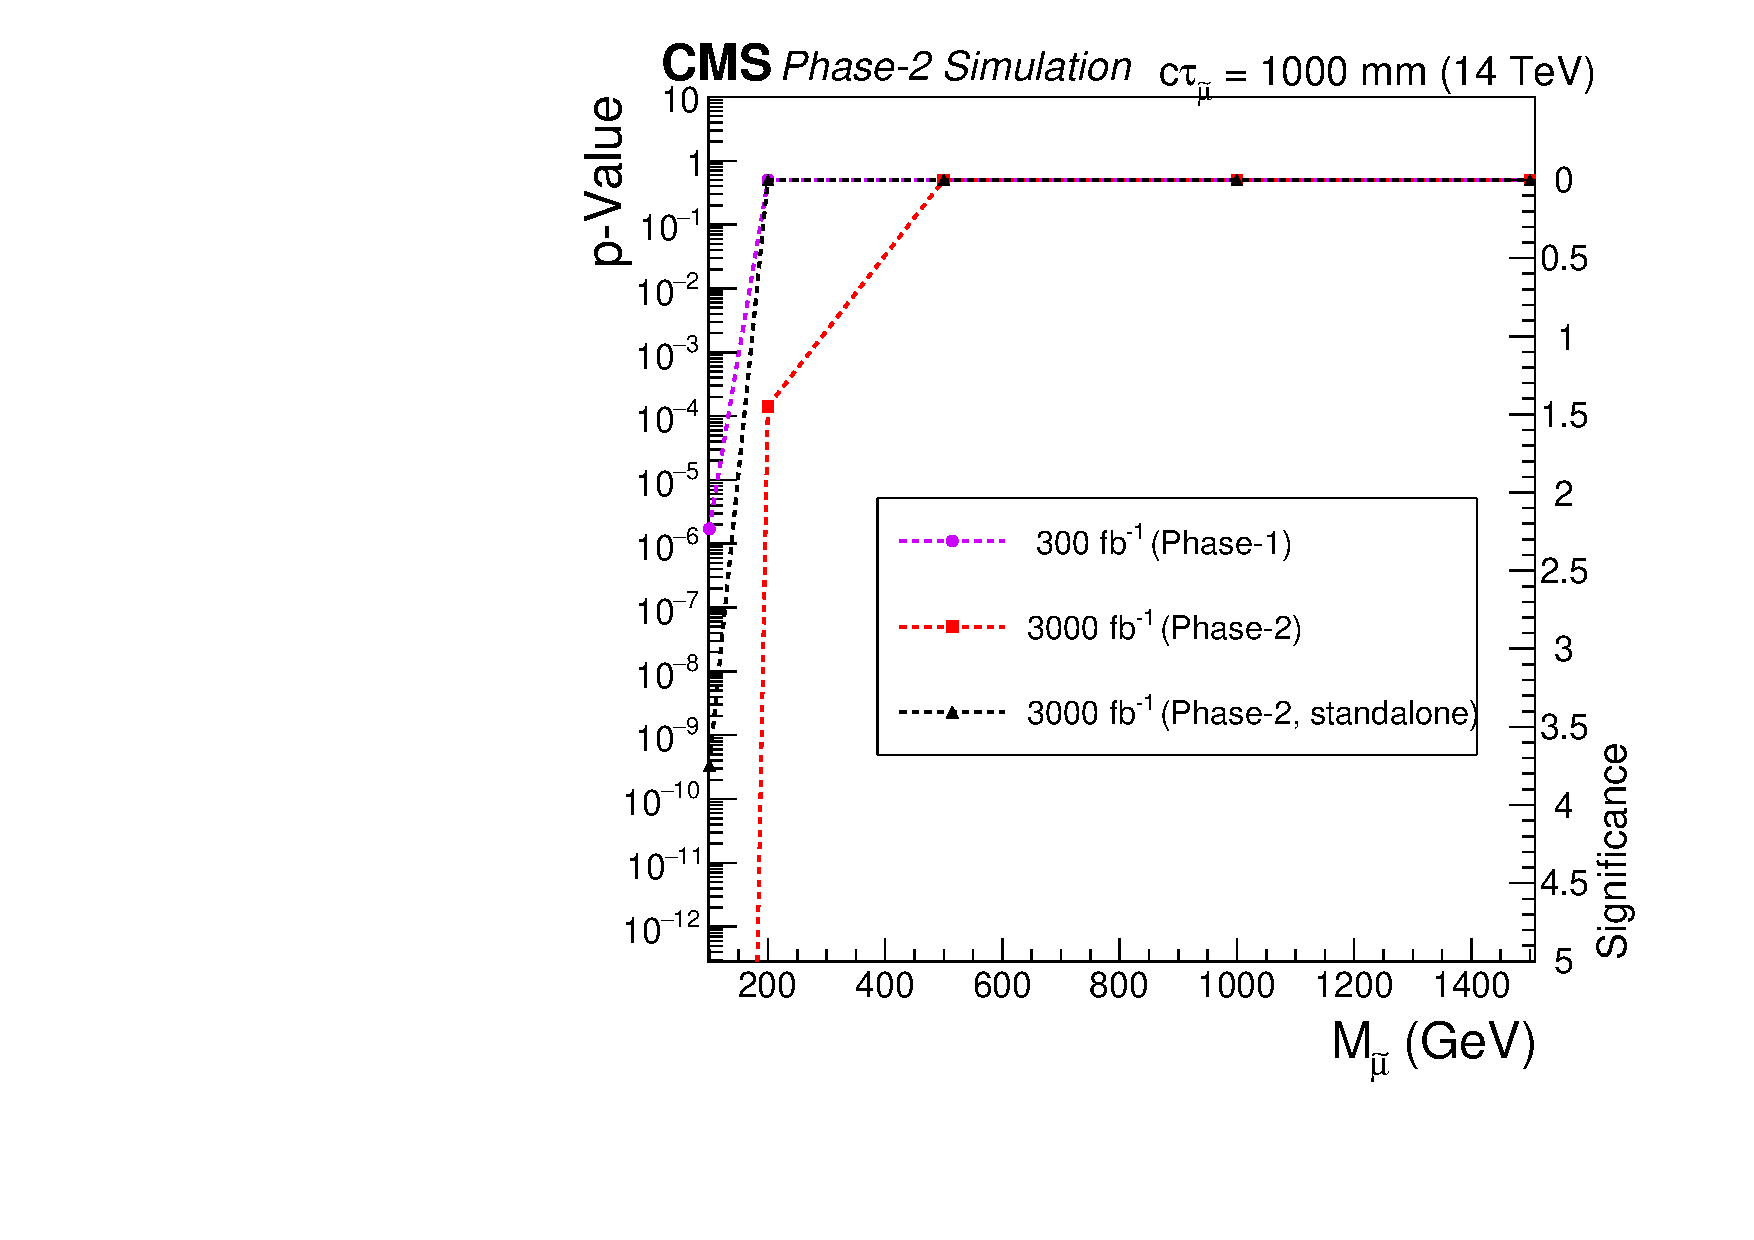
\includegraphics[width=0.47\textwidth]{figures/SignificanceComp.pdf}
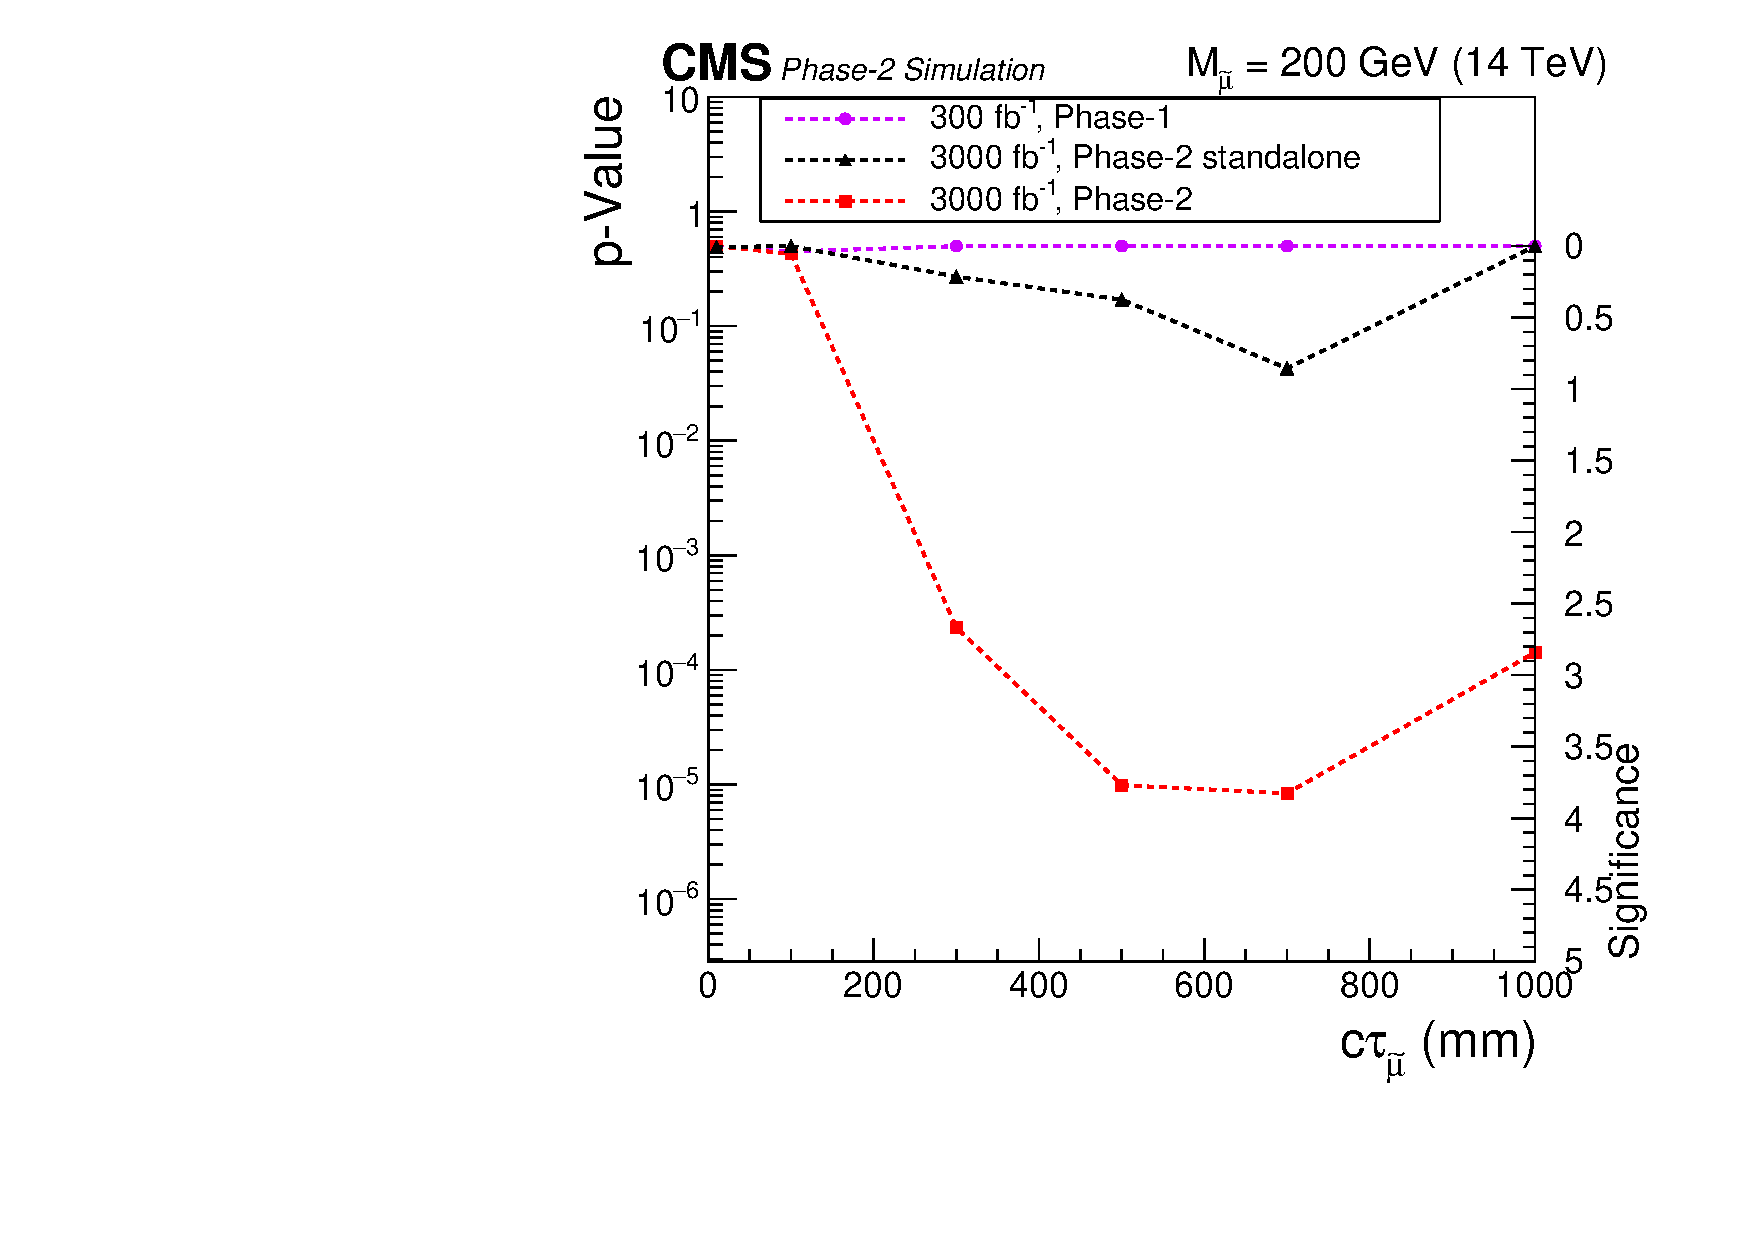
\includegraphics[width=0.47\textwidth]{figures/SignificanceComp_asfuncofCtau.pdf}
\caption{The projected discovery sensitivity at CMS for  $q \bar q \to \widetilde{\mu} \widetilde{\mu}, \widetilde{\mu}\rightarrow \mu\widetilde{G}$ for various mass hypotheses and $c\tau$ = 1~m (left) and as a function of the decay length for $m_{\widetilde{\mu}}$ = 200~GeV (right). Together with the discovery sensitivity the corresponding $p$-value is shown. Phase-2 results with an average of 200 pile-up interactions per bunch crossing and an integrated luminosity of 3000\fbinv are compared to results obtained with 300\fbinv. The black line shows the sensitivity without the DSA algorithm, which reduces the reconstruction efficiency by a factor three.
%NOT APPROVED!!! {\bf \textcolor{red}{[JB: It seems that the possibility of this plot being able to be shown publicly needs to be clarified.  Can our CMS colleagues look into it?]}} {\bf \textcolor{red}{[JA: All of these plots should be fine now.]}}
%~ In both panels, the theoretical cross section for the specific model is represented by the blue solid line.
%~ For different SUSY breaking scales, tan $\beta$ or otherwise modified parameters, the cross sections may be  100 times larger, reflected by the blue dash-dotted line.
%~ Green (yellow) shaded bands show the one (two) sigma range of variation of the expected 95\% CL limits. Phase-2 results with an average 200 pile-up events and an integrated luminosity of 3000\fbinv are compared to results obtained with 300\fbinv. The black line shows the sensitivity without the DSA algorithm, which reduces the reconstruction efficiency by a factor three.
%%% Drop discovery significance?
%c) Discovery sensitivity for various mass hypotheses. WORKING ON IT.
 }
\label{fig:displResultsSensitiviy}
\end{center}
\end{figure}


\paragraph{Sensitivity Projection with a Dark SUSY Model}
The analysis presented above was reinterpreted using a Dark SUSY model (\cite{Baumgart:2009tn,Falkowski:2010cm}), in which an additional dark $U_D(1)$ symmetry is added as a supersymmetric SM extension. Breaking this symmetry gives rise to an additional massive boson, the so-called dark photon ($\gamma_D$), which couples to SM particles via a small kinetic mixing parameter $\epsilon$. If $\epsilon$ is very weak, the lifetime of the dark photon can range from a few millimeters up to several meters. The lower $\epsilon$, the longer is the dark photon lifetime which then decays displaced from the primary vertex. A golden channel for such searches is the decay to displaced muons.

In the model studied here~\cite{CMS-PAS-FTR-18-002}, dark photons are produced in cascade decays of the SM Higgs boson that would first decay to a pair of MSSM-like lightest neutralinos ($n_1$), each of which can decay further to a dark sector neutralino ($n_D$) and the dark photon.

For the branching fraction BR$(H \to 2\gamma_D + \mathrm{X})$, where X denotes the particles produced in the decay of the SM Higgs boson apart
from the dark photons, $20\%$ is used. Neutralino masses $m(n_1) =
50~\mathrm{GeV}$ and $m(n_D) = 1~\mathrm{GeV}$ are assumed. Final states with two
and four muons are included in the analysis. In the former case, one dark photon decays to a pair of muons while the other dark photon decays
to some other fermions (2-muon final state). In the latter case, both dark photons decay to muon pairs (4-muon final state).

The main background for this search comes from multi-jet production (QCD), ttbar~production,
and Z/DY $\to\ell\ell$ events  where large impact parameters are (mis)reconstructed. Cosmic ray muons can travel through the detector far away from the primary vertex and mimic the signature of displaced muons.
However, thanks to their striking detector signature, muons from cosmic rays can be suppressed by rejecting back-to-back kinematics.

For each event, at least two DSA muons are required. If more than two, the ones with the
highest $p_T$ are chosen. The two muons must have opposite charge ($q_{\mu,1} \cdot q_{\mu,2} = -1$) and must be separated by $\Delta R = \sqrt{\Delta \phi^2 + \Delta
\eta^2} > 0.05$. The three-dimensional angle between the two displaced muons is required to be less than $\pi - 0.05$ (not back-to-back) in order to suppress cosmic
ray backgrounds. Additionally, $\ptmiss \geq 50~\mathrm{GeV}$ is imposed to account for the dark neutralinos escaping the detector without leaving any signal.

In order to discriminate between background and signal, the three-dimensional distance from the primary vertex to the point of closest approach of the extrapolated
displaced muon track, called $R_{\text{Muon}}$, is used.
The event yield after full event selection of both selected muons as a function of $R_{\rm Muon-1}$ and $R_{\rm Muon-2}$ is used to search for the signal. Figure\ref{fig:DarkPhoton_Distr_Disc}-left shows $R_{\rm Muon-1}$ of the first selected muon for signal and background samples.

\begin{figure}[hbtp]
\begin{center}
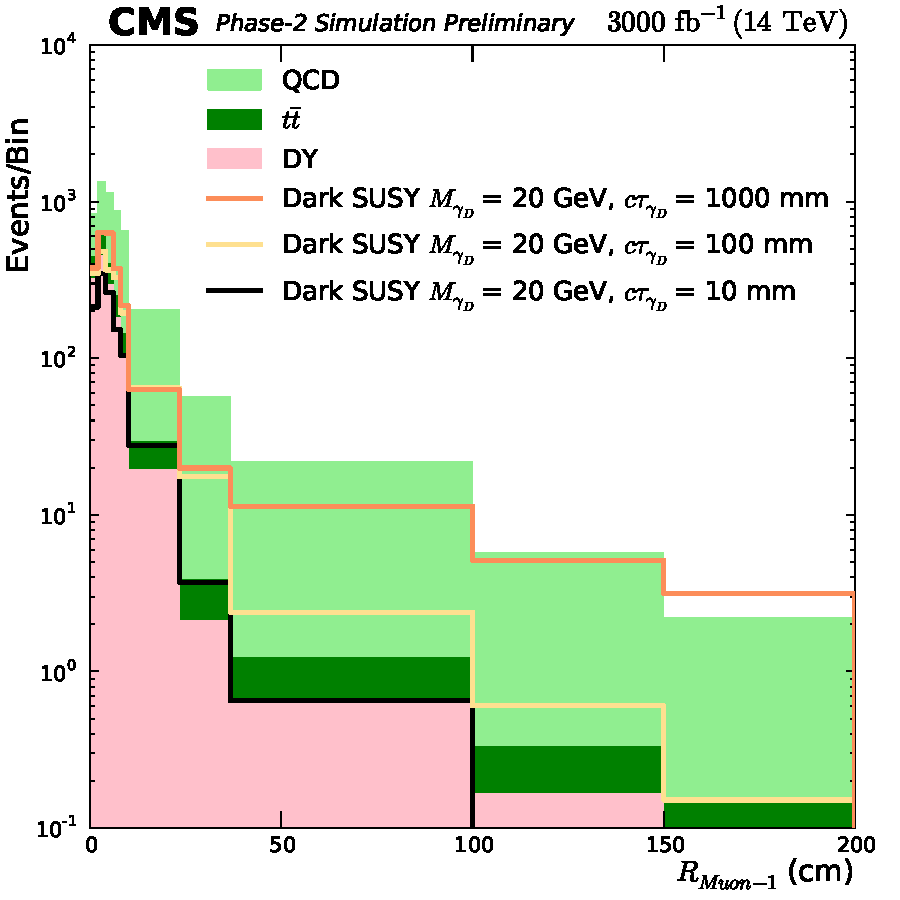
\includegraphics[width=0.45\textwidth]{tex/figures/cmsupgrade/FTR-18-002/DarkPhoton_Distribution}
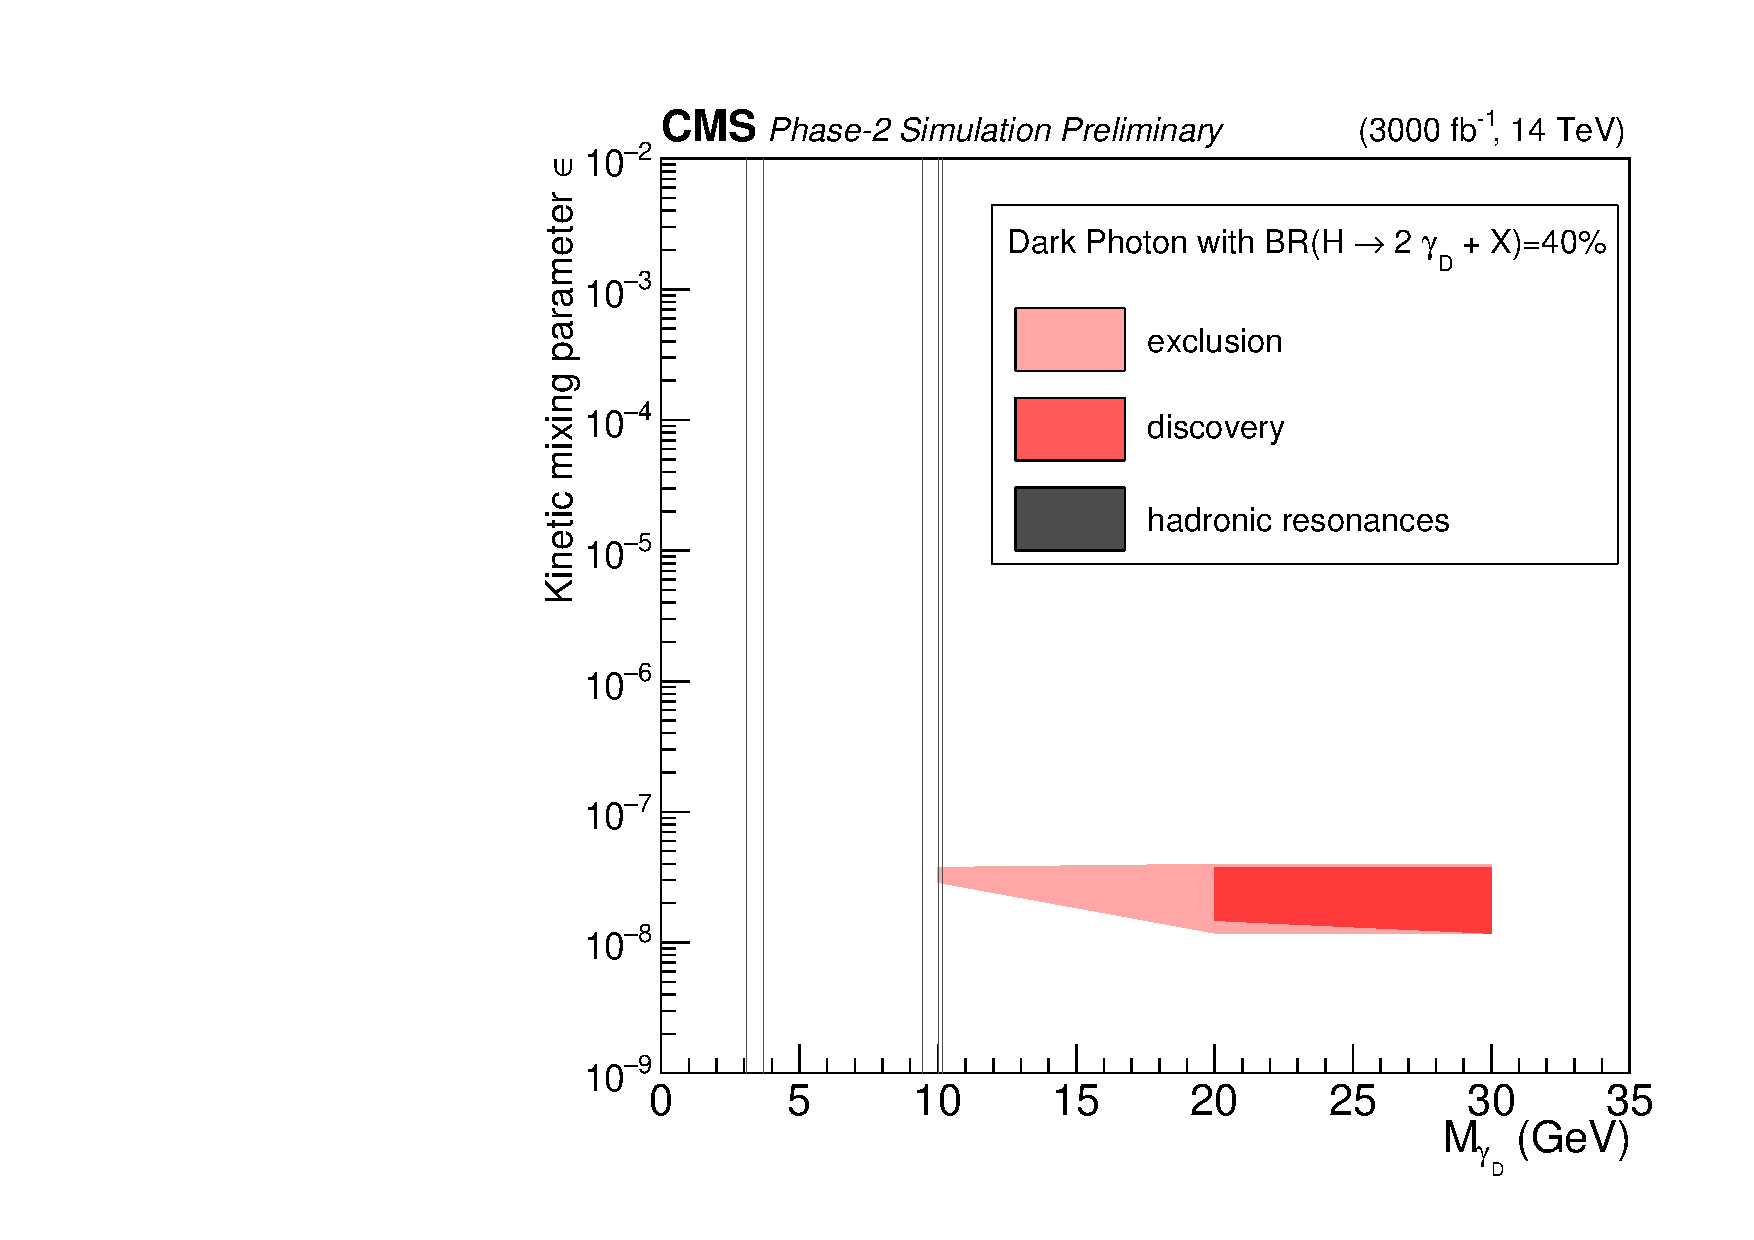
\includegraphics[width=0.45\textwidth]{tex/figures/cmsupgrade/FTR-18-002/Paramspace_merged.pdf}
 \caption{Left: Distance of the closest approach of the displaced muon track with maximum $p_T$  to the primary interaction vertex, $R_{\rm Muon-1}$, for signal and background after the final event selection.
Right:Parameter scan in the $\epsilon-m_{\gamma_D}$ plane. The grey lines indicate the regions of narrow hadronic resonances where the analysis does not claim any sensitivity.}
\label{fig:DarkPhoton_Distr_Disc}
\end{center}
\end{figure}


%%% Sensitivity in exclusion and discovery
The search is performed using a simple counting experiment approach. In presence of the expected signal, significance of the corresponding event excess over the expected background is assessed using the likelihood method.
In order to evaluate the discovery sensitivity the same input is used as in the limit calculation, now with the assumption that one would have such a signal in the data. The discovery sensitivity is shown in the two-dimensional $m_{\gamma_D}$-$c\tau$ plane
in Fig.~\ref{fig:DarkPhoton_Distr_Disc}-right. This search is sensitive to large decay length of the dark photon.

In absence of a signal, upper limits at $95\%$ confidence level (CL) are obtained on a signal
event yield with respect to the one expected for the considered model. A Bayesian method with a uniform prior for the signal event rate is used and the nuisance
parameters associated with the systematic uncertainties are modeled with log-normal distributions.
The resulting limits for the Dark SUSY models are depicted in Fig. \ref{fig:NewCompLimit_DarkPhoton}. While the results shown in Fig.\ref{fig:NewCompLimit_DarkPhoton}-left are for a dark photon with a decay length of $1~\mathrm{m}$ as a function of the dark photon mass, Fig.\ref{fig:NewCompLimit_DarkPhoton}-right shows the results for a dark photon mass of $20~\mathrm{GeV}$ as a function of the decay length~\cite{CMS-PAS-FTR-18-002}.



\begin{figure}[hbtp]
\begin{center}
\includegraphics[width=0.45\textwidth]{tex/figures/cmsupgrade/FTR-18-002/LimitComp_Ratio_DarkPhotons.pdf}
\includegraphics[width=0.45\textwidth]{tex/figures/cmsupgrade/FTR-18-002/LimitComp_Ratio_asfuncofCtau_DarkPhotons.pdf}
 \caption{Upper limits at $95\%$ CL on production cross section $\sigma / \sigma_{\text{theory}}$ for various dark photon mass hypotheses and a fixed decay length of $c\tau = 1000$~mm (a) and a fixed mass of $M_{\gamma_D} = 20$~GeV (b). Green and yellow shaded bands show the one and two sigma range of variation of the expected $95\%$ CL limits, respectively. The grey lines indicate the regions of narrow hadronic resonances where the analysis does not claim any sensitivity.}
\label{fig:NewCompLimit_DarkPhoton}
\end{center}
\end{figure}


\subsubsection{Displaced Photons at CMS}

%{\bf \textcolor{red}{[BS: Is it possible to explain the Lambda parameter in the GMSB model more in CMS displaced pohton section?]}}

A number of new physics scenarios predict new particles that, upon decay, result in displaced photons in the final state (see Sec.~\ref{sec:proposal} and Sec.~\ref{subsec:dphotons}). At the CMS experiment, with the scintillating crystal design of the ECAL that provides excellent resolution but lacks pointing capability, the photon arrival time in the ECAL is the main observable used to distinguish signal from background in displaced photon searches.

One benchmark model for displaced photon searches is the GMSB model where the lightest neutralino ($\tilde{\chi}_0^1$) is the next-to-lightest supersymmetric particle, can be long-lived, and decays to a photon and a gravitino ($\tilde{G}$), which is the LSP, as illustrated in Fig.~\ref{fig:cmsupgrade_photon} (left). For a long-lived neutralino, the photon from the $\tilde{\chi}_0^1\to\tilde{G}+\gamma$ decay is produced at the $\tilde{\chi}_0^1$ decay vertex, at some distance from the beam line, and reaches the detector at a time later than that of prompt, relativistic particles produced at the interaction point. The time of arrival of the photon at the detector can be used to discriminate the signal from the background. The aforementioned upgrade to the ECAL electronics in the barrel region, and the HGCAL upgrade in the endcaps, will improve photon timing resolution at HL-LHC by an order of magnitude to as little as $\sim30$~ps for photons with $p_T$ of tens of GeV or above, hence significantly improve the experimental reach of displaced photon searches.

Moreover, the proposed MIP Timing Detector (MTD) will be able to provide another dimension of information to reconstruct LLP decays. The time of flight of the photon inside the detector is the sum of the time of flight of the neutralino before its decay and the time of flight of the photon itself, until it reaches the detector. Since the neutralino is a massive particle the latter is clearly negligible with respect to the former. In order to be sensitive to short neutralino lifetimes of order 1~cm, the performance of the measurement of the photon time of flight is a crucial ingredient of the analysis. Therefore, the excellent resolution of the MTD apparatus can be exploited to determine with high accuracy the time of flight of the neutralino, and similarly the photon, also in case of a short lifetime.

An analysis has been performed at generator level in order to evaluate the sensitivity power of a search for displaced photons at CMS in the scenario where a 30~ps timing resolution is available from the MTD. The events were generated with Pythia 8~\cite{Sjostrand:2007gs}, exploring neutralino lifetimes ($c\tau$) in the range 0.1--300~cm. The values of the $\Lambda$ scale parameter, which controls the ??,%{\bf \textcolor{red}{[JB: Word missing.]}}
were considered in the range 100--500 TeV, which is relevant for this model to be consistent with the observation of a 125~GeV Higgs boson. After requiring the neutralino to decay within the CMS ECAL acceptance and the photon energy being above a ``trigger-like'' threshold, the generator-level photon time of flight was smeared according to the expected experimental resolutions. A cutoff at a photon time greater than 3$\sigma$ of the timing resolution is applied and the ``signal region'' is assumed to be background free to estimate the sensitivity. The signal efficiency of such a requirement is computed and translated, assuming the theoretical cross sections provided in Ref.~\cite{Strassler:2006im}, to an upper limit, at 95\% CL, on the production cross section of the $\tilde{\chi}_0^1 \to \tilde{G} + \gamma$ process.

In Figure~\ref{fig:cmsupgrade_photon} (right), the analysis sensitivity in terms of the $\Lambda$ scale (and therefore of the neutralino mass) and lifetime is shown for three different assumptions on the timing resolution. The 300~ps resolution is representative of the time-of-flight resolution (TOF) consistent with current CMS detector performance. The 180~ps resolution is representative of the TOF resolution of the upgraded CMS detector without the MTD, in which case the TOF measurement will be dominated by the time spread of the luminous region. The vertex timing provided by the MTD detector will bring the TOF resolution to about 30~ps. As visible in the figure, a full-scope upgrade of the CMS detector with photon and track timing will provide a dramatic increase in sensitivity at short lifetimes and high masses, even with the first $300\,\,\mathrm{fb}^{-1}$ of integrated luminosity.

\begin{figure}[t]\begin{center}
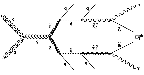
\includegraphics[width=0.47\textwidth]{figures/MTD/diagram.pdf}
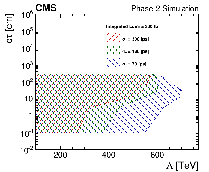
\includegraphics[width=0.47\textwidth]{figures/MTD/Limits_excl_2D_ComparingRes.pdf}
\caption{
Left: Diagrams for a SUSY process that results in a diphoton final state through gluino production at the LHC. Right: Sensitivity to GMSB $\tilde{\chi}_0^1 \to \tilde{G} + \gamma$ signals expressed in terms of neutralino lifetimes for 300, 180 and 30~ps resolution, corresponding to the current detector, the HL-LHC detector with photon timing without MTD and with MTD, respectively.
}
\label{fig:cmsupgrade_photon}
\end{center}
\end{figure}

\subsubsection{Displaced Jets in ATLAS}

%{\bf \textcolor{red}{[JB: Can this section be expanded a bit?  The discussion assumes a lot of knowledge that will be unclear to someone not in ATLAS.]}}

Neutral long-lived particles that can decay into jets displaced from the proton-proton interaction point arise in many BSM theories (see Chapter~\ref{sec:simplifiedmodel} for an extensive discussion). For example, in hidden sector models a new set of particles and forces is proposed that is weakly coupled to the SM via a communicator particle. The hidden sector is otherwise invisible to the SM sector, but its particles (some of which can be long-lived) may decay to SM particles via the communicator. The lifetimes of these LLPs are typically unconstrained and could be long enough for the LLPs to decay inside the ATLAS detector volume. Such particles produce unique signatures which may have been overlooked by more traditional searches for new physics. One ATLAS search for such displaced jet signatures focuses on LLPs which decay in the ATLAS hadronic calorimeter (HCal) and consequently deposit most of their energy there and very little or none in the electromagnetic calorimeter, and also have few or no charged tracks pointing at the hadronic energy deposits. A signature-driven trigger that optimizes the acceptance for this class of events is required for the online selection.

The existing ATLAS analysis described in Sec.~\ref{subsec:djets} can likely be improved by planned upgrades by using HCal information splitting the B-C layers in the calorimeter to identify the LLP decay position. %{\bf \textcolor{red}{[JB: What are the B-C layers?  Are they something new for the upgrade?  How does this change from now till upgrade time?]}}
The splitting between B-C layers will provide more information on the longitudinal shower profile, see~Figure~\ref{fig:Caloratio}.

This analysis uses a hidden sector benchmark model and considers the decay of a heavy boson to two long-lived neutral scalars; this maps to the simplified model with Higgs boson production of hadronically decaying LLPs in Sec.~\ref{sec:proposal}. The heavy scalar bosons decaying into LLPs have masses ranging from 125 GeV to 1000 GeV, and the LLP scalars have masses ranging between 5 GeV and 400 GeV.
Background processes, dominated by QCD dijet production, are suppressed in this analysis by requiring both scalars to decay both in the calorimeter.

\begin{figure}[hbtp]
\begin{center}
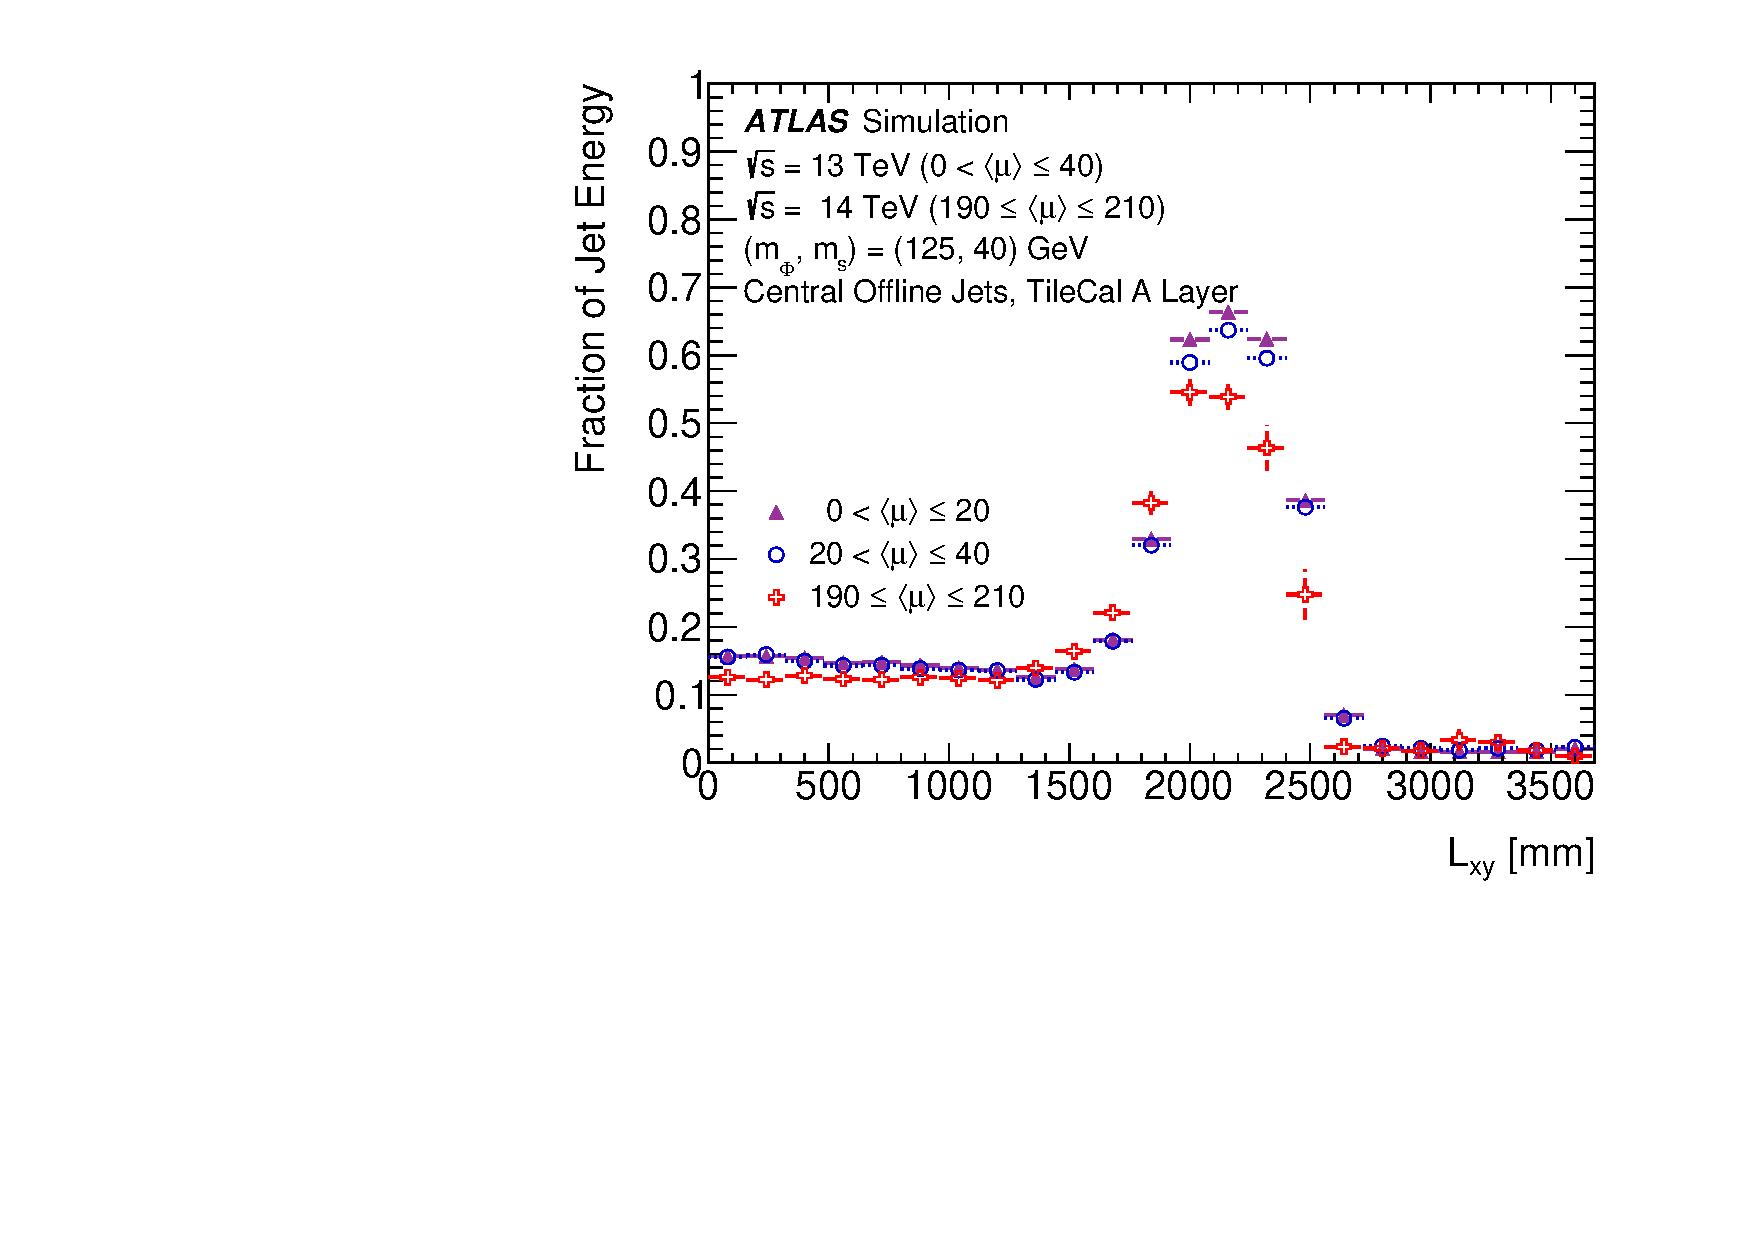
\includegraphics[width=0.47\textwidth]{figures/caloratio1.pdf}
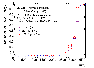
\includegraphics[width=0.47\textwidth]{figures/caloratio2.pdf}\\
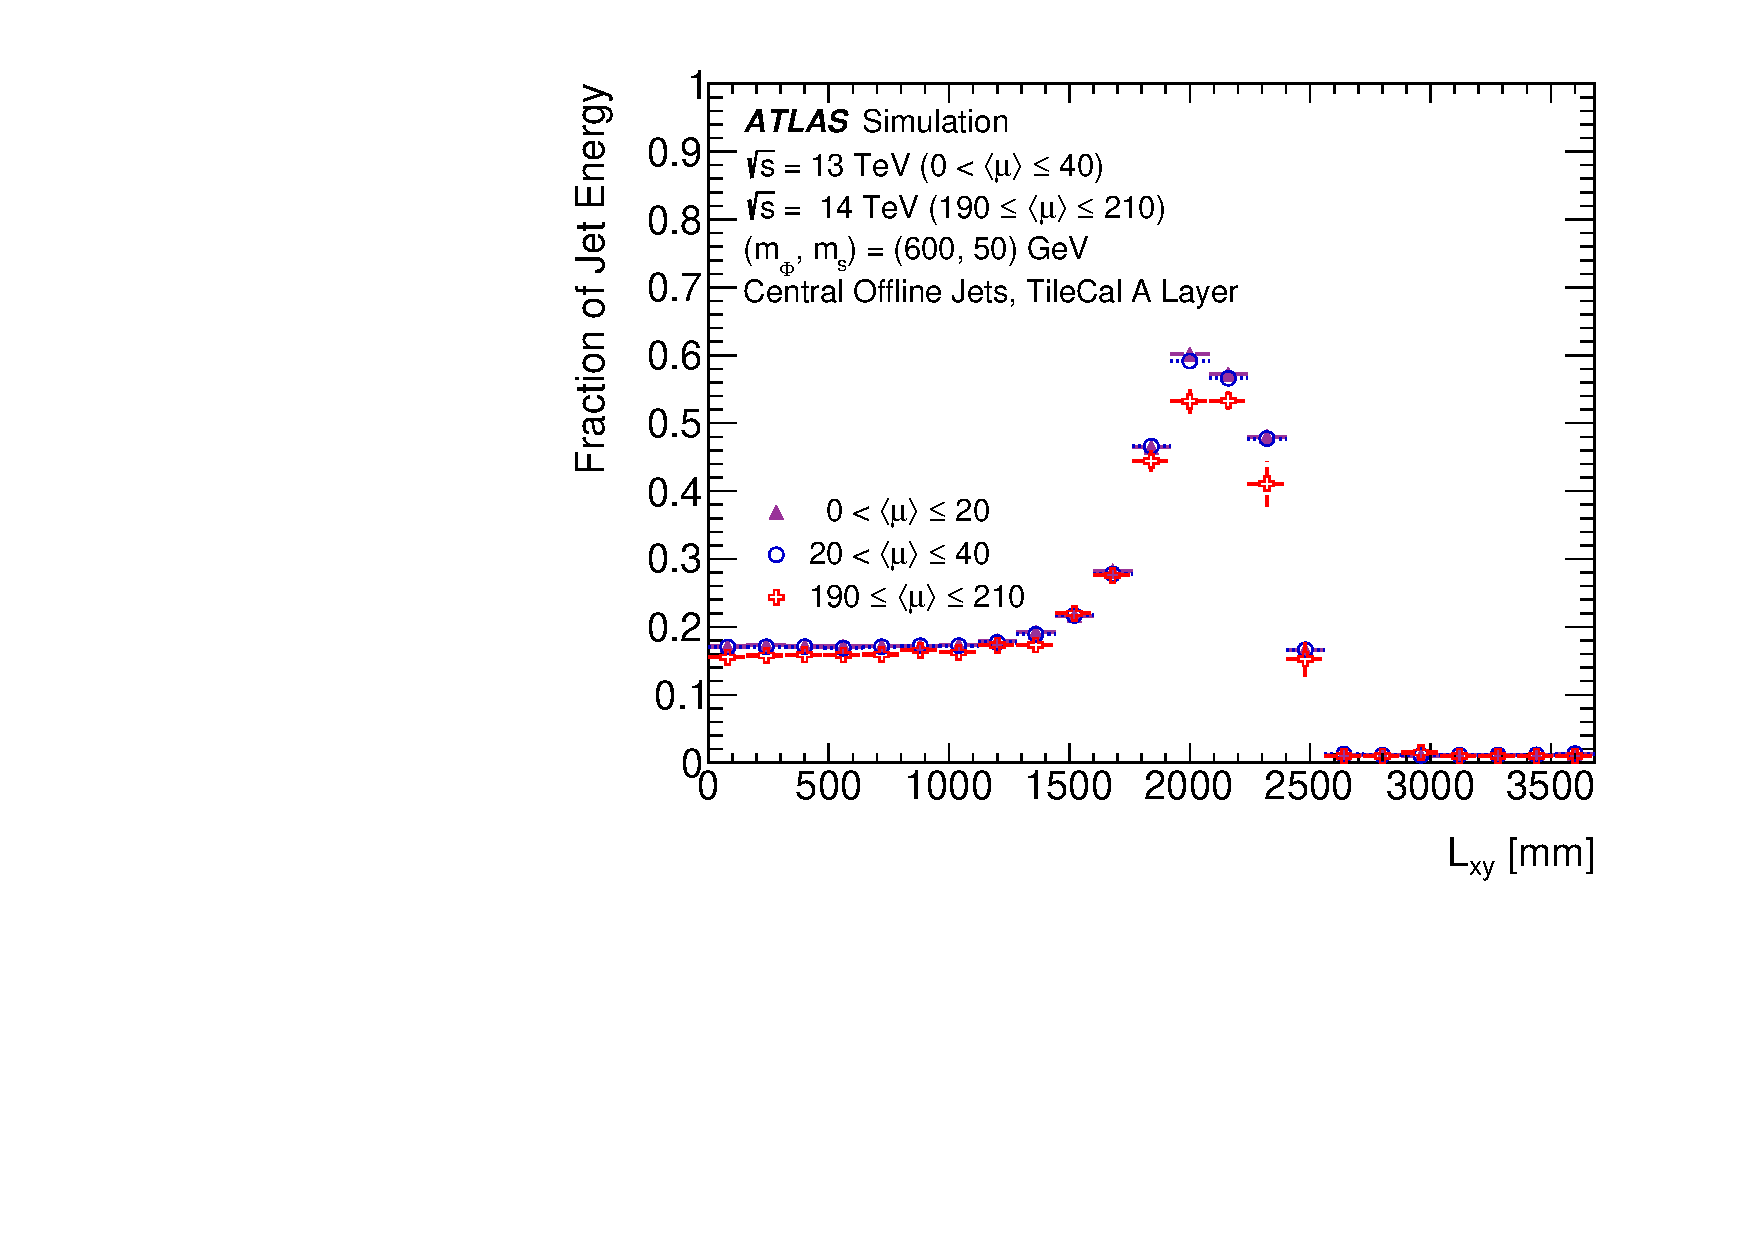
\includegraphics[width=0.47\textwidth]{figures/caloratio3.pdf}
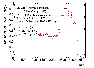
\includegraphics[width=0.47\textwidth]{figures/caloratio4.pdf}\\
\caption{ %{\bf \textcolor{red}{[JB: Can this be described?  What are these plots?]}}
}
\label{fig:Caloratio}
\end{center}
\end{figure}

%\noindent {\bf \textcolor{red}{[BS: This section kind of just ends after the figure. What is the outcome of the study?]}}

\subsubsection{Disappearing Tracks}

In the ATLAS experiment, the planned ITk upgrade of the tracking volume for the HL-LHC can be exploited to improve the existing searches for BSM particles with a disappearing track.

Such particles are predicted by many well-motivated supersymmetric models such as anomaly-mediated SUSY-breaking scenarios, where the supersymmetric partners of the Standard Model $W$ bosons, the wino fermions, are the lightest SUSY state. In such models, the lightest neutralino and chargino can be nearly mass-degenerate, with a mass splitting around 160~MeV. When produced in a high-energy collider, the chargino can acquire a relatively long lifetime,%{\bf \textcolor{red}{[JB: Does the chargino acquire the long lifetime from the high-energy collider?]}}
and leave multiple hits in the traversed tracking layers before decaying. When performing searches for such signatures in ATLAS, selected events are typically required to contain at least one short track, hereafter called a tracklet. To study how such searches can be improved with the ITk upgrade, some assumptions have been made for simulating events and projected detector response. The detector response is parametrised by using response functions based on studies performed with Geant4 simulations of the upgraded detector in high-luminosity pile-up conditions.

The tracklet reconstruction efficiency for signal charginos as a function of the decay radius inside the detector is shown in Figure~\ref{fig:ATLAS_DT1}. A 30\% systematic uncertainty on the background yields is assumed, as observed for the Run 2 analysis. The expected background is largely dominated by fake tracklets. %{\bf \textcolor{red}{[JB: Fake tracklets from what?]}}
%
\begin{figure}[t]\begin{center}

\includegraphics[width=0.9\textwidth]{figures/ch03_fig_039.pdf}
\caption{ %{\bf \textcolor{red}{[JB: Can this be described?  What is this plot?]}}
}
\label{fig:ATLAS_DT1}
\end{center}
\end{figure}

Expected limits at 95\% CL are shown in Figure~\ref{fig:ATLAS_DT2} as a function of the chargino mass and lifetime for a pure wino and a pure higgsino LSP scenario. For comparison, the current Run 2 limit for 36.1 ${\rm fb}^{-1}$ in the wino LSP scenario is also shown. The HL-LHC dataset of 3000 ${\rm fb}^{-1}$ extends the sensitivity of neutrinos and charginos up to 250~GeV, assuming a pure higgsino scenario.

%
\begin{figure}[t]\begin{center}

\includegraphics[width=0.47\textwidth]{figures/ch03_fig_040a.pdf}

\includegraphics[width=0.47\textwidth]{figures/ch03_fig_040b.pdf}

\caption{ %{\bf \textcolor{red}{[JB: Can this be described?  What are these plots?]}}
}
\label{fig:ATLAS_DT2}
\end{center}
\end{figure}

\subsubsection{Displaced Vertices in ATLAS}

Massive, long-lived particles with lifetimes of the order of O(10) ps to O(10) ns can decay inside the inner tracker into charged and stable particles. The products of these decays are reconstructed as tracks with measurably distant impact parameters with respect to the IP. The reconstruction of such displaced tracks is very challenging compared to the track reconstruction of prompt particles, due to fewer hits along the track and a larger parameter phase space for track finding. %{\bf \textcolor{red}{[JB: This is a good initial discussion of displaced tracking but this is the section about identifying displaced vertices, yes?  How do the two relate?]}}

Several physics models predict the existence of long-lived, massive particles. For example, a standard SUSY scenario can contain a gluino with a mass of 2~TeV and a lifetime of 1~ns. The long-lived gluino hadronises into an R-hadron, which decays into a 100~GeV neutralino and hadrons.

In ATLAS, this topology has been investigated in Run 2 by using a dedicated algorithm for reconstructing displaced vertices. The performance expected to be achieved for the ITk upgrade for this signal has been tested with a simplified simulation which has a description of the ITk active sensors and a modeling of the magnetic field. The kinematics and location of the decay products of the R-hadron are injected into the simulation and their trajectories are extrapolated through the detector model. The probability of producing at least seven silicon hits in the ITk geometry is tested.

%{\bf \textcolor{red}{[JB: What are we to conclude from this discussion?  Is anything public?  Can we show a plot?  If not, can we describe in words, even roughly, whether the sensitivity for this search is expected to improve with upgrades?]}}

\subsubsection{LLP searches with precision timing at CMS}

%{\bf \textcolor{red}{[BS: Are the track resolutions in mm or microns?! Seems like it should be microns.]}}
%{\bf \textcolor{red}{[JA: Yes, should have been microns. Fixed.]}}

The CMS MTD will provide new, powerful information in searches for long-lived particles. In addition to the aforementioned displaced photon search, the additional timing information can be used to provide full kinematic reconstruction of LLP decays, and can be a powerful tool in background suppression.

\paragraph{Possible improvements in the ability to reconstruct LLP mass}

A precision MIP timing detector allows each reconstructed vertex to be assigned a time and therefore to measure the time of flight of LLPs between primary and secondary vertices. Using the measured displacement between primary and secondary vertices in space and time, the velocity of an LLP in the laboratory frame, $\vec{\beta}_{LAB}^{p}$ (or, equivalently, the boost $\gamma^p$), can be measured. In such scenarios, the LLP can decay to fully visible or partially invisible systems. Using the measured energy and momentum of the visible portion of the decay, one can calculate its energy in the LLP rest frame and reconstruct the mass of the LLP, assuming that the mass of the invisible system is known.

This capability can be demonstrated in scenarios where the LLP decay produces a $Z$ boson, which then decays to an electron-positron pair. For example, in the GMSB model where the $\tilde{\chi}_0^1$ couples to the gravitino $\tilde{G}$ via higher-dimension operators sensitive to the SUSY breaking scale, the $\tilde{\chi}_0^1$ may have a long lifetime, and can be produced in top-squark pair production with $\tilde{t}\to t+\tilde{\chi}_0^1$, $\tilde{\chi}_0^1 \to Z+\tilde{G}$, $Z\to ee$.

Studies with simulated event samples have been performed to estimate the possible improved sensitivity of the search with the CMS MTD upgrade. The events are generated with Pythia 8, and the masses of the top-squark and neutralino are set to 1000~GeV and 700~GeV, respectively. Generator-level quantities are smeared according to the expected experimental resolutions. A position resolution of $12\,\,\mu\mathrm{m}$ in each of the three spatial directions is assumed for the primary vertex. The secondary vertex position for the electron-positron pair is reconstructed assuming $30\,\,\mu\mathrm{m}$ position resolution in the transverse direction. The momentum resolution for electrons is assumed to be $2\%$. Finally, the time resolution of charged tracks at the displaced vertex is assumed to be 30~ps.

The mass of the LLP is reconstructed assuming that the gravitino is massless. The fraction of events with separation between primary and secondary vertices exceeding 3$\sigma$ in both space and time as a function of the MTD resolution is shown in Figure~\ref{fig:cmsupgrade_mtd} (left). The mass resolution, defined as half of the shortest mass interval that contains $68\%$ of events with 3$\sigma$ displacement is shown in Figure~\ref{fig:cmsupgrade_mtd} (right), as a function of the MTD resolution.

\begin{figure}[t]\begin{center}
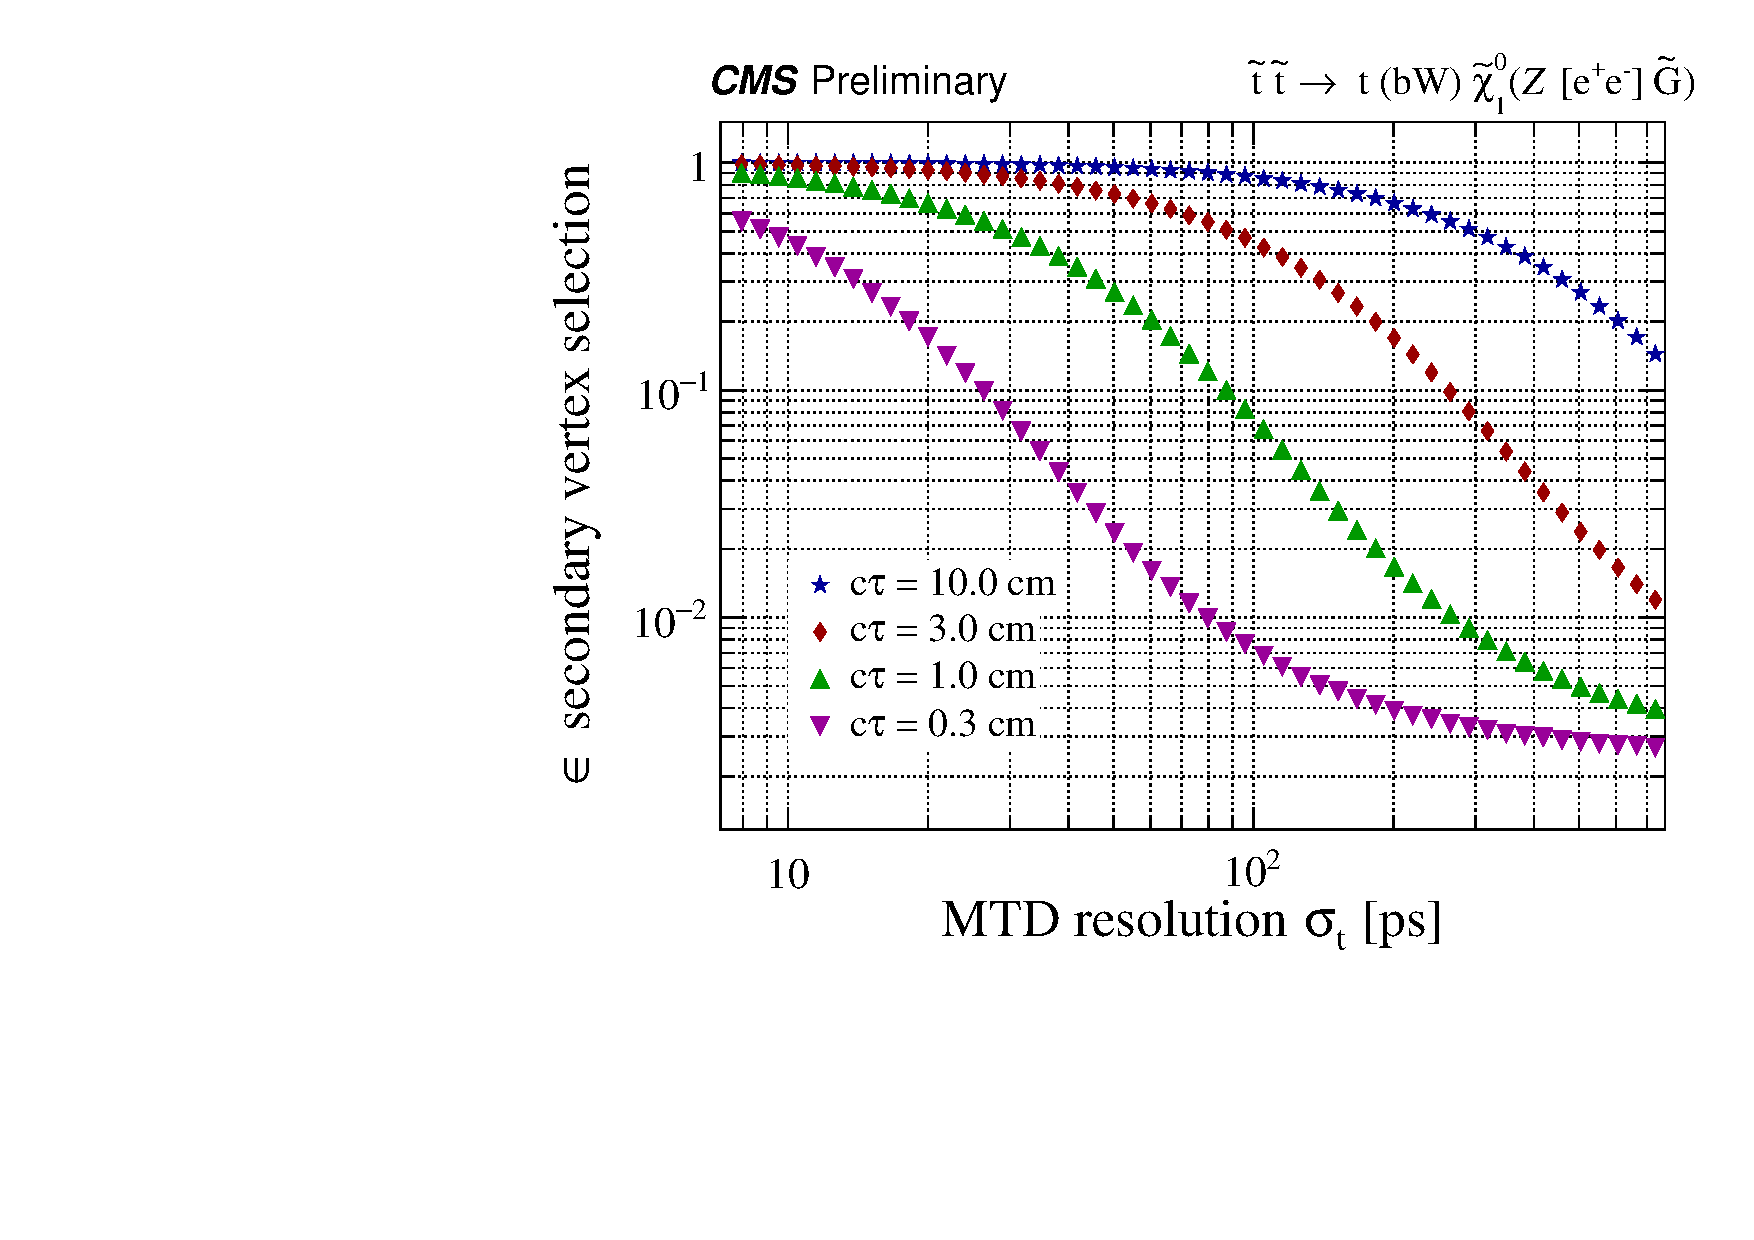
\includegraphics[width=0.47\textwidth]{figures/MTD/171025_52.pdf}
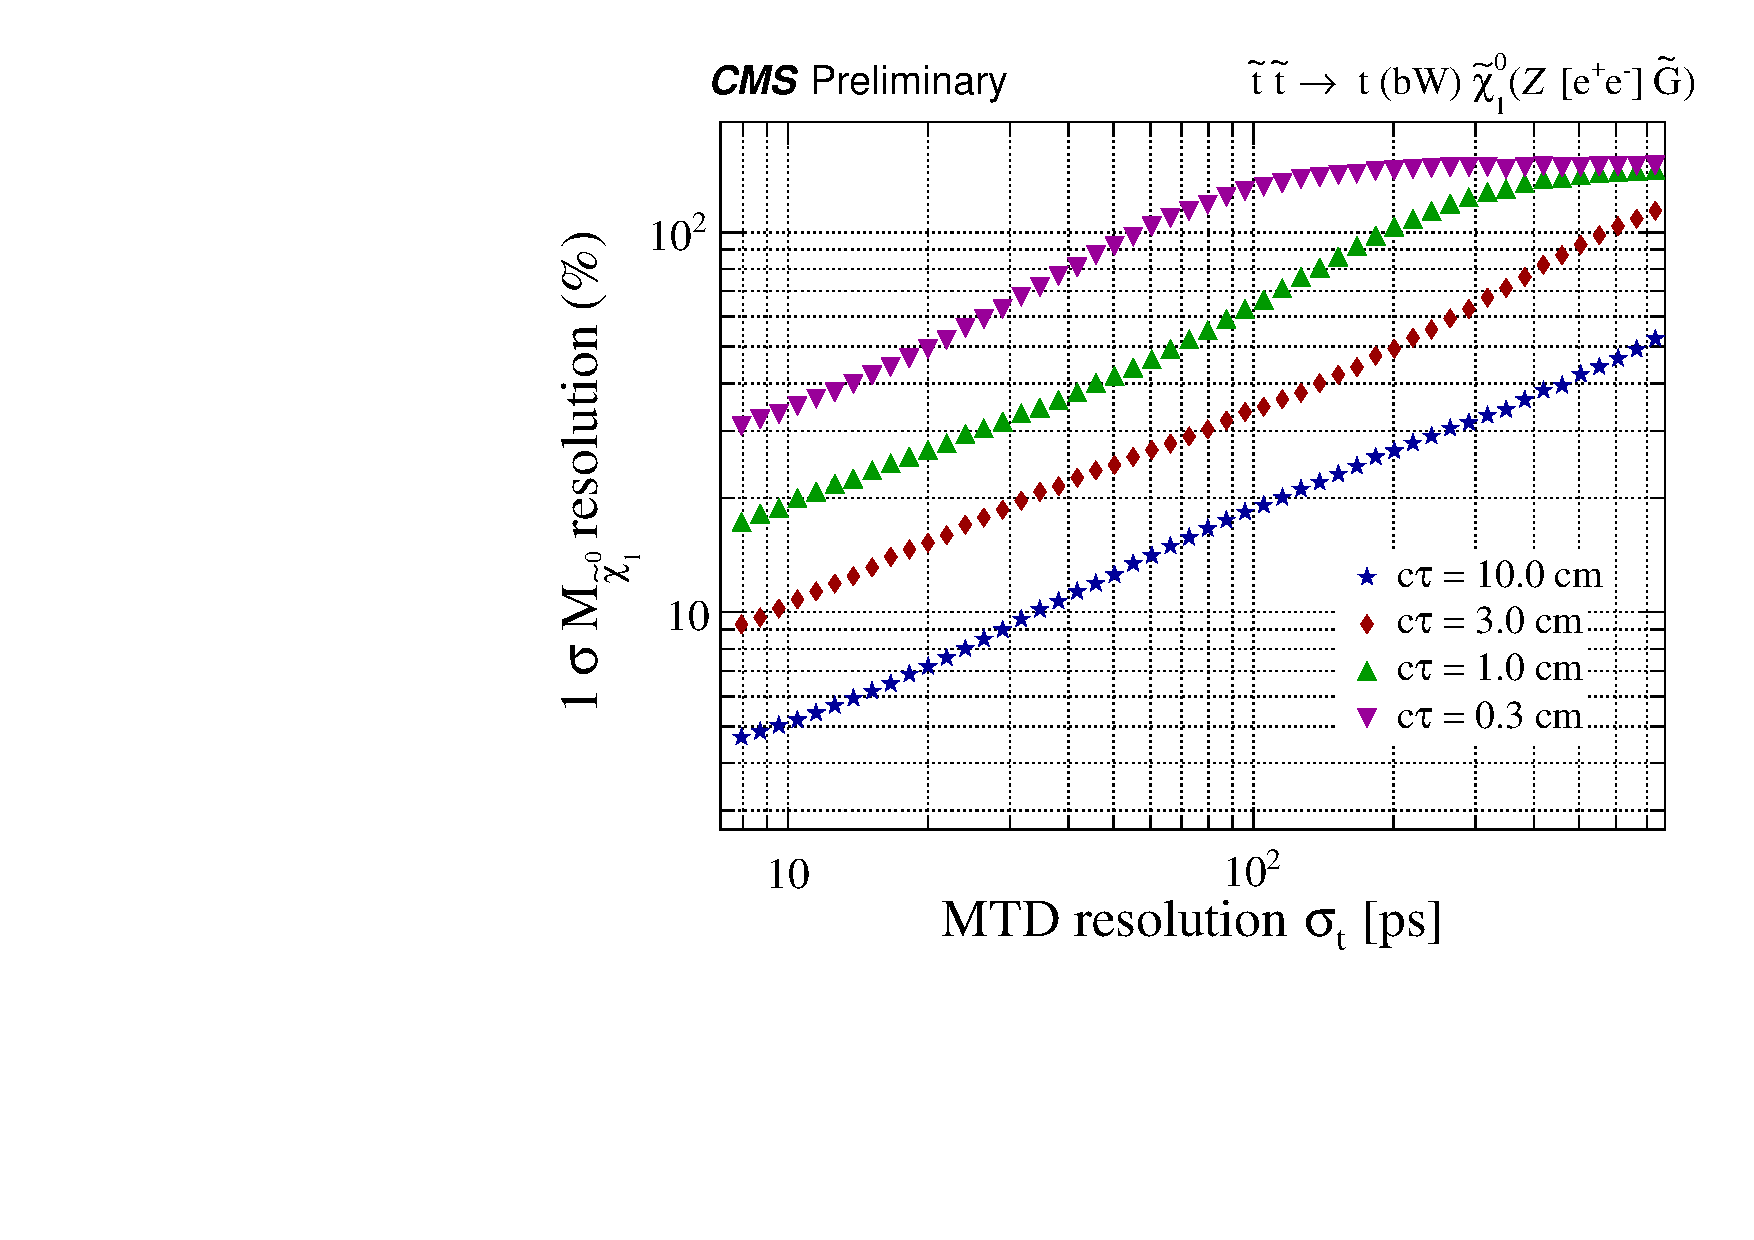
\includegraphics[width=0.47\textwidth]{figures/MTD/171025_53.pdf}
\caption{
Efficiency (left) and mass resolution (right) as a function of the timing resolution of the MTD for reconstruction of the $\tilde{\chi}_0^1$ mass in the SUSY GMSB example of $\tilde{\chi}_0^1 \to \tilde{G} e^{+} e^{-}$, with mass of $\tilde{\chi}_0^1=700$~GeV, considering events with a separation of primary and secondary vertices by more than $3\sigma$ in both space and time.
}
\label{fig:cmsupgrade_mtd}
\end{center}
\end{figure}

A similar study has been performed with another SUSY scenario where the two lightest neutralinos and light chargino are higgsino-like. The light charginos and neutralinos are nearly mass degenerate and may become long-lived as a consequence of the heavy higgsinos. In both studies, the additional timing information from the MTD facilitates the reconstruction of the LLP mass, the resolution and efficiency of which are further improved with the excellent timing resolution of the MTD.

%\noindent {\bf \textcolor{red}{[JB: Can we add a brief, unambiguous statement about whether the upgrade will provide improvement?]}}

%\noindent {\bf \textcolor{red}{[BS: Are there any results for the Higgsino example? Should we just leave it out?]}}

\paragraph{Possible improvement to LLPs searches in general using timing information}

Precision timing at CMS will provide a new tool to suppress the background and enhance the reach for LLPs in the HL-LHC era.
\begin{figure}[htb]
    \centering
    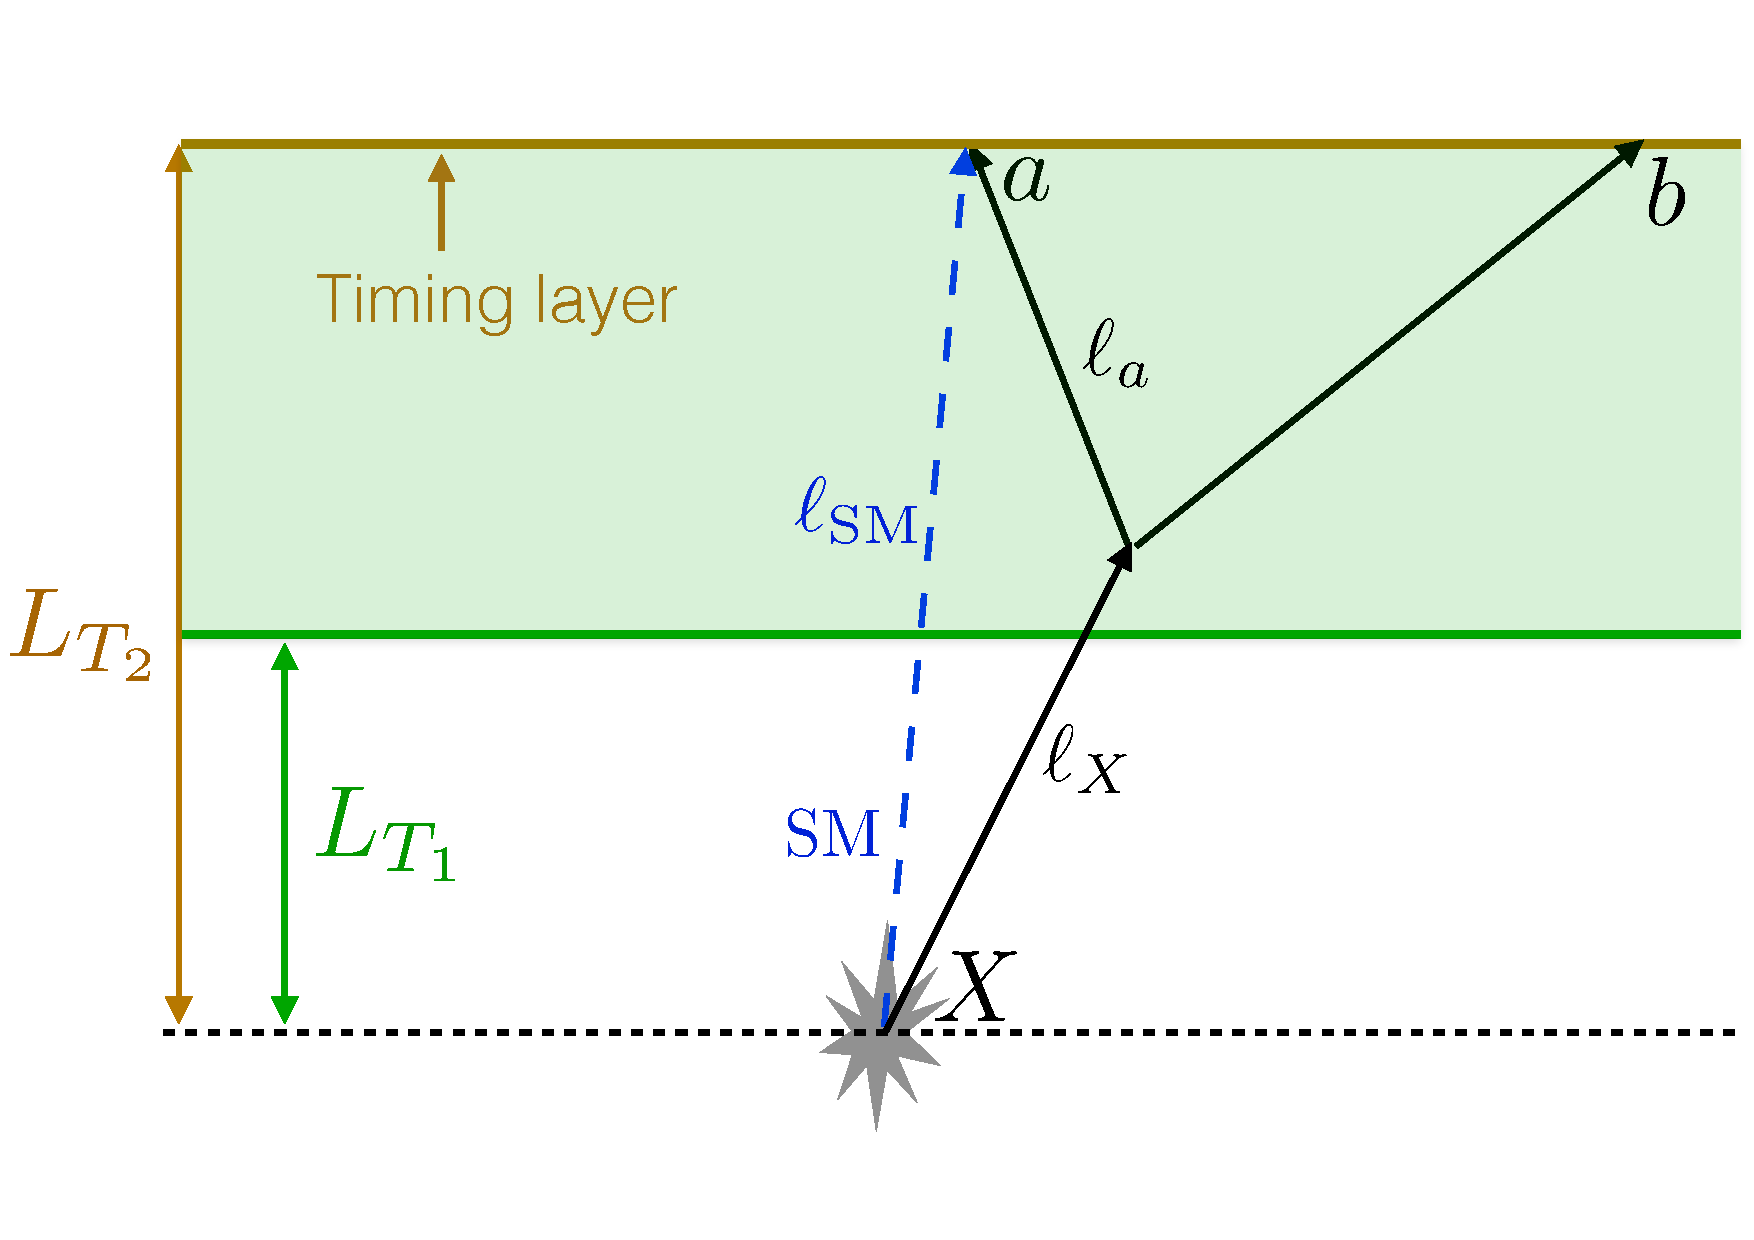
\includegraphics[width=0.9\columnwidth]{figures/MTD/schematic_drawing.pdf}
    \caption{An event topology with an LLP $X$ decaying to two light SM particles $a$ and $b$. A timing layer, at a transverse distance $L_{T_2}$ away from the beam axis (horizontal gray dotted line), is placed at the end of the detector volume (shaded region). The trajectory of a potential SM background particle is also shown (blue dashed line). The gray polygon indicates the primary vertex. Taken from Ref.~\cite{Liu:2018wte}}
    \label{fig:drawing}
\end{figure}

A schematic of a typical signal event containing an LLP is shown in Figure~\ref{fig:drawing}. An LLP, denoted as $X$, travels a distance $\ell_X$ into a detector volume and decays into two light SM particles $a$ and $b$, which then reach a timing layer at a transverse distance $L_{T_2}$ away from the beam axis. In a typical hard collision, the SM particles generally travel very close to the speed of light. Hence, the decay products of $X$ (using particle $a$ as an example) arrives at the timing layer with a time delay of
\beq
 \Delta t = \frac{\ell_X}{\beta_X} + \frac{\ell_a}{\beta_a} - \frac{\ell_{\rm SM}}{\beta_{\rm SM}},
\label{eq:delaysimple}
\eeq
with $\beta_a \simeq \beta_{\rm SM} \simeq 1$. An ISR jet could easily be present for all processes, and can be used to ``timestamp'', i.e., to derive the time of the hard collision at the primary vertex.

For the CMS MTD located just outside the tracker volume, ${\ell_{\rm SM}}/{\beta_{\rm SM}}$ is about $O(1\,\,\mathrm{ns})$. As a result, with tens of picosecond (ps) timing resolution, a sensitivity to percent-level time delay caused by slow LLP motion, e.g., $1-\beta_X>0.01$ with boost factor $\gamma<7$, is expected to be achieved.

A new trigger strategy for a delayed jet can be realized by comparing the prompt jet with $p_T > 30$~GeV that reconstructs the four-dimensional primary vertex (PV4d) with the arrival time of another jet at the timing layer. The delayed and displaced jet signal, after requiring a minimal decay transverse distance of 0.2~m ($L_{T_1}$), will typically not have good tracks associated with it. Consequently, the major SM background is from trackless jets. The origins of this background can be classified into two categories: same-vertex (SV) hard collision and pile-up (PU).

% The SV background for such signals mainly comes from SM multi-jet processes. At least one prompt jet is required to reconstruct the PV4d and provide the timestamp, while another trackless jet from the same hard collision can then mimic a long-lived signal decay. At 13~TeV, with integrated luminosity $\mathcal{L}_{\rm int} = 3~\text{ab}^{-1}$, the total number of such background events can be estimated as
% \begin{align}
% N_{\rm bkg}^{\rm SV} = \sigma_{\rm multi-jet} \mathcal{L}_{\rm int} {\epsilon_{\rm trig}{\epsilon_{\rm j, fake}}}
% \approx 5.6 \times 10^{9}  \nonumber
% \label{eq:bkgQCDforHC}
% \end{align}
% where $\sigma_{\rm j} \approx 3.7 \times 10^6$~pb is the multi-jet cross-section with $p_{T,j} > 30$~GeV, and $\epsilon_{\rm trig}$ and $ \epsilon_{\rm j, fake}$ are the efficiencies for the background to fake the signal in both triggering and signature {\bf \textcolor{red}{[JB: What does it mean for the background to fake the signal ``in signature''?]}} {\it without} timing information.

The fake jet has an intrinsic time delay $\Delta t=0$. However, due to the limited timing resolution in reconstructing the PV4d, it could have a time spread. The background differential distribution with respect to apparent delay time ($\Delta t$) can be estimated as
\beq
\frac {\partial N_{\rm bkg}(t)^{\rm SV}} {\partial \Delta t }= N_{\rm bkg}^{\rm SV}
\mathcal{P} (\Delta t;\delta_t^{\rm PT}).
\label{eq:bkgSV}
\eeq
The time delay cut on $\Delta t$ reduces such background through the tiny factor of $\mathcal{P}(\Delta t;\delta_t^{\rm PT})$ for large $\Delta t/\delta^{\rm PT}_t$.
% if $\Delta t/\delta^{\rm PT}_t$ is greater than a few.
% {\bf \textcolor{red}{[JB: A few what?]}}. Zhen: this ratio is a dimensionless quantity...
The LLP signal pays a much smaller penalty factor than the background due to its intrinsic delay.

The background from the pile-up requires the coincidence of a triggered hard event and objects from a pile-up (hard) collision whose PV4d fails to be reconstructed and that can mimic a signal. The differential background from pile-up can be estimated as
\beq
\frac {\partial N^{\rm PU}_{\rm bkg}(\Delta t)} {\partial \Delta t} \simeq N_{\rm bkg}^{\rm PU}
{\mathcal P}(\Delta t;\delta_t^{\rm PU}).
\label{eq:bkgPU}
\eeq
The key difference between the background from the pile-up and the background from the same hard collision is that the typical time spread is determined by the beam property for the former, and by the timing resolution for the latter. They typically differ by a factor of a few, e.g., 190~ps versus 30~ps for CMS with the current upgrade plan.
%If we apply the requirement $\Delta t > 0.8$~ns, the total estimated number of events from SM background including SV and PU is minimal at a calculated value of 0.33 {\bf \textcolor{red}{[JB: This is for what luminosity?  This number is to be compared to what other number?]}}.
%Zhen: I don't think we need to discuss such details here we can just refer back to the original paper.

Using this estimation, a sensitivity projection is presented with an example signal of a Higgs boson decaying to an LLP with the subsequent decay of the LLP into $b \bar b$ pairs, with only minimal requirements of one low-$p_T$ ISR jet, with $p_{T,j} > 30$~GeV and $|\eta_j| < 2.5$, and at least one LLP decay inside the detector. Timing information is used to suppress background. The $95\%$ C.L. sensitivity is shown in Figure~\ref{fig:ctaulimitHiggs}. The decay branching ratio of the LLP $X \to j j$ is assumed to be $100\%$. The projection with $30$~ps timing resolution of the CMS MTD (labeled EC), is plotted with thick dashed lines. Compared to other 13 TeV HL-LHC projections (with $3 ~\text{ab}^{-1}$ of integrated luminosity) without the timing information (shown in thinner, dotted and dashed lines), it is seen that the addition of a timing cut greatly reduces background and improves sensitivity. The significant improvement from the theory work Ref.~\cite{Liu:2018wte} using timing upgrades inspires many experimental and phenomenological studies to fully realize the physics potential in LLP searches using precision timing information at the HL-LHC.

%\noindent {\bf \textcolor{red}{[BS: This is a theorist projection. Too optimistic? Maybe include at the end and clarify that this is simply a theory interpretation of a possibility. Or maybe we leave it out?]}}
%Zhen: added a sentence above to stress it is a theoretical work. Since this is a chapter about upgrades, I think it is fully justified to show our projections.

\begin{figure}[ht]
    \centering
    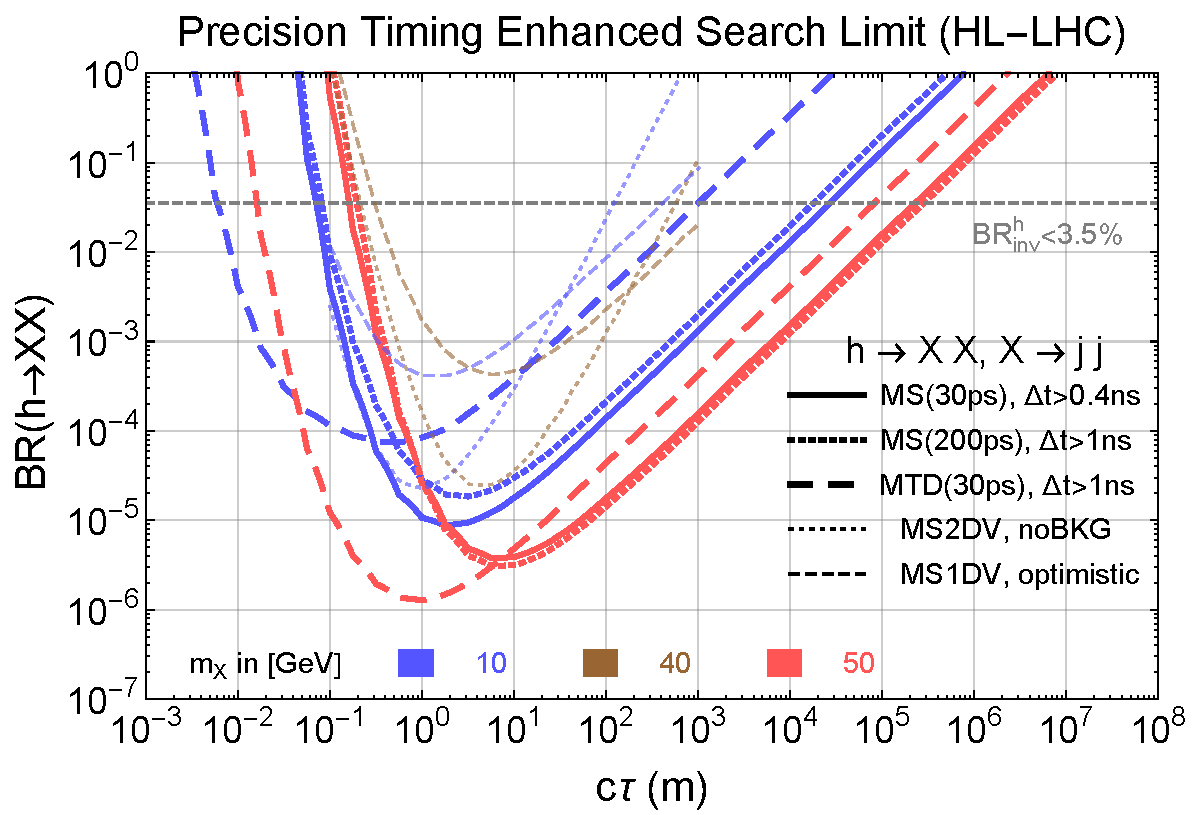
\includegraphics[width=1.0\columnwidth]{figures/MTD/10-20-50-MC-Lcalc-BRlimit-with-deltaT-cut-MS-1ns.pdf}
    \caption{The $95\%$ C.L. limit on $\text{BR}(h \to XX)$, where $X$ is an LLP, for the production of $pp \to j h$ with the subsequent decay of $h\to X X$ and $X \to j j$. Different colors indicate different masses of the particle $X$. The thick, long-dashed lines indicate searches with the CMS MTD plus the timing requirements. The thick solid and dotted lines indicate searches with a hypothetical timing layer outside the ATLAS muon spectrometer plus timing requirements. The numbers in parentheses are the assumed timing resolutions. Taken from Ref.~\cite{Liu:2018wte}}
    \label{fig:ctaulimitHiggs}
\end{figure}

\subsubsection{LLP searches with a Level-1 track trigger in CMS}

%{\bf \textcolor{red}{[BS: Missing citation to CMS TOY upgrade tracker geometry.]}}

As discussed in Section~\ref{sec:upgrademachine}, a central feature of the CMS upgrade at the HL-LHC will be a new silicon outer tracker which allows track reconstruction for every LHC bunch crossing (at a rate of 40~MHz). The $p_T$ selection for stubs (hit pairs in the $p_T$ modules of the outer tracker) to be read out is determined by the bandwidth from the detector to the back end electronics, and is fixed at about 2~GeV. On the other hand, the choice of track finding algorithm and hardware is still being finalized, and there could be significant benefits to extending the L1 track trigger capabilities to trigger on off-pointing tracks.

To illustrate the case, a simple toy simulation to study rare Higgs boson decays into new particles with lifetimes of order of a few mm has been performed~\cite{Gershtein:2017tsv}. This study considers all-hadronic final states with low $H_T$, taking SM Higgs boson decays into four jets as an example. Theoretical motivation to look for such decays is very strong; see Section~\ref{sec:motivated_theories} for a detailed discussion. The goal is to probe very small branching fractions of the Higgs boson, so for these studies $BR[h\rightarrow\phi\phi\rightarrow 4q] = 10^{-5}$ is assumed. For prompt decays, the background is overwhelming, but if the $\phi$ has $c\tau$ of a few mm, the offline analysis has very low backgrounds. The problem is getting such events on tape, in particular through L1. This toy study estimates how an off-pointing track reconstruction at L1 can help. To estimate the efficacy of the approach, the resulting projections are compared with the best alternatives in the absence of an off-pointing track trigger, by using associated Higgs boson production with a $W$ boson that decays leptonically to pass a lepton trigger, or considering L1 calorimeter jets with no associated prompt tracks.

This study is performed by utilizing a simulation with a toy tracker which has six perfectly cylindrical double layers~\cite{geom} %{\bf \textcolor{red}{[JB: Reference missing.]}}
covering $|\eta|<2.4$. For each layer, the allowed offset between the two measurements is below the one expected from 2~GeV prompt tracks. The sketch in Figure~\ref{fig:tracktrigger_toy} (left) shows four tracks traversing a double layer: positively and negatively charged
prompt 2~GeV tracks, and two off-pointing tracks. The dashed track would make a L1 trigger stub, and the dotted one would not.

Two extensions of the track finder are considered. {\it Loose} tracks are only required to have a minimal number of stubs. {\it Tight} tracks are obtained by fitting the stubs they produce to a circle constrained to the beam line. The number of stubs on a tight track is the number of stubs deviating from that circular fit by fewer than three strips (300 microns). This choice of definition of ``tight'' tracks is a generous approximation for an algorithm that assumes prompt production when building a track and allows for a non-zero impact parameter for the track fit. For loose tracks, both track building and fitting assumes a non-zero impact parameter. Only the transverse plane of the track-finding is considered since that is the plane in which the displacement is measured more precisely. It is also assumed that the hits on a track are additionally linked in $rz$, but this assumption is not relied upon for the calculation of displacement.

The $h\rightarrow\phi\phi\rightarrow 4q$ events are generated using Pythia. The mass of the LLP, $\phi$, is taken to be 30~GeV, and $Br[h\rightarrow\phi\phi\rightarrow 4q]=10^{-5}$. A range of $\phi$ lifetimes is considered, from 1~mm to 5~m. Proper decay times are randomly generated for each $\phi$ and time dilation effects are included.

In Figure~\ref{fig:tracktrigger_toy} (right), the expected event yields are shown for the different triggers described above. Jet reconstruction parameters are slightly varied to ensure there are no large variations in efficiency. For track jets, one (solid lines) or two (dashed lines) tracks with five or more hits are required. For trackless jets, one track (solid line) or two tracks with total $p_T$ below 10~GeV is/are allowed to point along the jet.

While the tight tracks offer a substantial increase in sensitivity compared to $Wh$, a trigger based on loose tracks yields more than a factor of five more signal for $c\tau$ of a few mm. Trackless jets, even with very optimistic 70~GeV threshold only become competitive at lifetimes of 50~cm or more.

\begin{figure}[t]\begin{center}
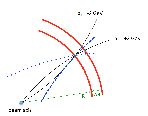
\includegraphics[width=0.47\textwidth]{figures/L1TT/geom.pdf}
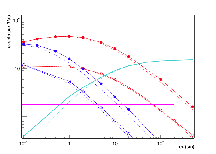
\includegraphics[width=0.47\textwidth]{figures/L1TT/final_h125.pdf}
\caption{Left: Sketch of the toy stub formation in a doublet layer in the context of a possible CMS track trigger for the HL-LHC. Four tracks pass through the same point in the inner layer. Only the tracks hitting the outer layer between the two green points would produce a L1 stub. The dashed track does, and the dotted does not. Right: Event yields for $Br[h\rightarrow\phi\phi\rightarrow 4q]=10^{-5}$ as a function of $\phi$ proper lifetime. Red curves correspond to a trigger that requires at least four loose track jets and blue to a trigger that requires at least four tight track jets. Open circles indicate track jets with $p_T$ above 20~GeV and filled circles to displaced track jets above 10~GeV. The teal curve corresponds to the no-track, 70~GeV di-jet trigger. The purple line shows the expected yield from $Wh$ production triggered by a lepton from the $W$ decay.}
\label{fig:tracktrigger_toy}
\end{center}
\end{figure}

The rare SM Higgs boson decay considered above is challenging to probe at the LHC because of the small total $H_T$ in the event (see Sec.~\ref{sec:covgaps}). While Higgs boson-like signals may be accessible when produced in association with leptonically decaying vector bosons, some new physics signals may not. As an example, hidden sector models where LLPs are produced through particles other than the Higgs boson may not give rise to $VH$ production modes. These LLP signals will greatly benefit from the displaced track trigger studied here.

\subsection{Open Questions and New Ideas}\label{sec:upgradeideas}

%\textbf{TBA}: coordinate with ATLAS \& theory

The higher data rate and more powerful machinery in the high-luminosity era bring new prospects to LLP searches. Searches that are too challenging for the current machine may become feasible with the HL-LHC upgrades, and it is important to explore such possibilities to the full extent. Existing search methods, triggering, and reconstruction algorithms should also be updated to take full advantage of the new hardware capabilities. As the upgrade scope is being defined and finalized in the near future, it is of particular importance to evaluate the physics cases, which will also motivate the upgrade and inform its designs.

\subsubsection{New studies for the HL-LHC}

In Sec.~\ref{sec:upgradesearch}, various analyses with displaced signatures are presented in the context of how detector and trigger upgrades at the ATLAS and CMS experiments for the HL-LHC can improve their sensitivity. As was shown in Sec.~\ref{sec:upgrademachine}, while the upgrades for both experiments differ in detail, they are similar in concept and scope. It is therefore important to perform the same LLP search projections for both experiments to compare performance and evaluate the complementarity of the two experiments.

For example, both experiments explore the idea of a fast timing detector at HL-LHC. The CMS MTD aims for full-coverage of a barrel layer plus endcap disks, while the ATLAS HGTD plans for multiple layers of endcaps. How the different $\eta$ coverage of the timing layer might impact LLP searches will be an interesting question to answer. In the case of calorimetry, the ATLAS LAr electromagnetic calorimeter is segmented in $z$, providing the additional pointing capability to find displaced photons. On the other hand, the CMS ECAL electronics upgrade in the barrel, and HGCAL upgrade in the endcaps, will considerably improve its timing resolution to identify photons that are out-of-time. A sensitivity comparison of both experiments will provide helpful information in understanding photon reconstruction and the combined reach of both experiments.

Furthermore, as new models are being proposed and new channels open up in the realm of LLP searches, many with final states challenging for the current detector conditions, it is important to evaluate their sensitivities in the high luminosity era. Here are a few of such interesting searches that are on the agenda.

\begin{itemize}
\item \textbf{Inelastic dark matter}

While stringent limits are currently placed on WIMP-type dark matter from direct detection, indirect detection, and collider searches, dark matter particles can exist in a hidden sector with additional particles and forces. A representative example of a hidden sector consists of a dark matter particle which is charged under a hidden gauge or global symmetry. The DM can have both a symmetry-preserving mass and, if the symmetry is spontaneously broken, also a symmetry-violating mass, which splits the mass eigenstates. This inelastic dark matter (iDM) scenario~\cite{TuckerSmith:2001hy,Bai:2011jg,Izaguirre:2015zva} consists of two DM states that couple only off-diagonally to one another. Such iDM can be probed at colliders with the production of $\mathrm{DM}+\mathrm{DM}^*$ (where $\mathrm{DM}^*$ denotes the heavier DM state) in association with a hard SM object $X$, followed by the subsequent decay of $\mathrm{DM^*}\rightarrow\mathrm{DM} +Y$ for some potentially different SM states $Y$. The production is summarized as
\begin{eqnarray} \label{eq:schematic-production}
pp  &\to&   X +  \mathrm{DM}+\mathrm{DM}^*   \nonumber \\     &\to&  X + \mathrm{DM}+ \biggl( \mathrm{DM}^* \to \mathrm{DM}+  { Y}\biggr)     \equiv  X + \slashed{E}_{\rm T}+ Y ~,~ \nonumber
\end{eqnarray}
where $X$ is any state that can be used to trigger on the event and reconstruct $\slashed{E}_{\rm T}$, such as an ISR jet, and $Y$ depends on the mode by which DM couples inelastically to the SM.

One concrete, representative version of such models can be realized when the mediator is a dark photon and $Y$ is a pair of leptons. The weak coupling between the SM and the hidden sector suggest the heavy eigenstate is meta-stable, creating a displaced signature. Because the mass splitting is small between the two eigenstates, the lepton pair is also typically softer compared with GMSB models, with $p_T$ values of a few to tens of GeV for a $O(10\,\,\mathrm{GeV})$ DM. The displaced muon trigger and reconstruction strategy with the muon system upgrade at CMS can likely improve searches for this scenario. The soft $p_T$ spectrum in this case particularly motivates the lowering of the $p_T$ threshold in the displaced muon trigger turn-on. Moreover, the additional timing information from the fast-timing detector opens up the possibility of reconstructing the mass splitting, while taking advantage of the good resolution of the timing detector for even low-$p_T$ particles. Sensitivity studies for iDM with a dark photon mediator are planned for the CMS MTD upgrade. The projections will also be of value to searches for other types of dark sector models, such as self-interacting dark matter~\cite{Hochberg:2014dra}, that give rise to soft displaced lepton pairs. %{\bf \textcolor{red}{[JB: Can our ATLAS colleagues add a similar discussion about their upgrade potential here?]}}

\item \textbf{Dark showers}

If the hidden sector has a QCD-like structure with dark quarks and hidden forces, a mediator between the SM and the hidden sector, such as a $Z'$ or heavy Higgs boson, can decay into some number of dark quarks that subsequently shower and hadronize into dark mesons, some of which are meta-stable and decay back into SM particles after a macroscopic distance from the proton-proton interaction point. A showering dark sector can yield a particularly rich collider phenomenology that may give rise to a high multiplicity of displaced objects often low in $p_T$. Depending on the final state, searches for a hadronic shower with emerging~\cite{Schwaller:2015gea} or semi-visible~\cite{Cohen:2015toa} jets can be improved with the increased acceptance and enhanced resolution due to the tracker upgrades at both ATLAS and CMS, as well as the finer granularity endcap calorimeter (HGCAL) at CMS. A dark shower with displaced photon pairs can benefit from the improved timing resolution with the ECAL electronics upgrade, as well as the new timing detectors. A dark shower with displaced lepton pairs, similar to the aforementioned case of inelastic dark matter, can be probed with better sensitivity with the muon system upgrades, as well as the fast timing information. For more details on dark showers, see Chapter~\ref{sec:showers}.

\item \textbf{Long-lived stop searches with fast timing}
TBA with Caltech input

\item \textbf{Boosted object reconstruction with fast timing}
TBA with input from Matt Klimek

\item \textbf{Others}: More!
\end{itemize}

\subsubsection{New detectors at future collider}

If we are only limited by our imagination, what new detectors may exist at a future collider that can open up new capabilities for LLP searches? Regardless of practical constraints, studies for such bold new proposals also help us understand our current experimental reach and optimize our search strategies.

\begin{itemize}
\item \textbf{4-dimensional tracker with timing}

Extending from the ``timing layer'' approach for HL-LHC upgrades, it is clear more time measurements on the track are favorable. In particular, time-of-flight between layers is a powerful discriminant for choosing hits on a track. A future tracker that provides 4-dimensional information, including precise timing information for every layer, can significantly improve track reconstruction by reducing combinatorics, providing purer track seeds, and remove fake stubs. Assuming high-$p_T$ particles, each layer's time measurement is advanced by 30~ps and so preserves the differences in vertex times. Low $p_T$ particles will have even more discrimination power since their paths leave longer times between hits in consecutive layers of the tracker.

Major technical advances will need to happen to achieve such an implementation, including development of fine-pitch sensors with good timing resolution, improvements in scaling and power consumption, electronics upgrade, and alterations to present pattern recognition methods in track finding.

\item \textbf{Timing detector outside ATLAS Muon System}

As discussed in Sec.~\ref{sec:upgradesearch}, by using a prompt object, such as an ISR jet, to ``timestamp'' an event, and cutting on the timing delay from the LLP, the new timing layer (MTD) at CMS can help significantly reduce the background and improve LLP search sensitivity. The CMS MTD is located between the tracker and the ECAL with a distance to the beamline of about $1.2\,\,\mathrm{m}$. If one imagines a fast timing layer outside the ATLAS muon system (MS) with a distance of approximately $10\,\,\mathrm{m}$~\cite{Liu:2018wte}, timing information at such distances could provide additional discriminating power for particles with longer lifetimes. In Figure~\ref{fig:ctaulimitHiggs}, the projection with a $30$~ps timing resolution of such a hypothetical detector outside the ATLAS muon system is plotted in a thick solid line. A less-precise timing resolution ($150$~ps) has been also considered with a cut $\Delta t > 1$~ns to suppress background. The LLP efficiency is largely unaffected by this change, while low-mass LLPs lose sensitivity by a factor of a few.

The CMS MTD timing upgrade for the HL-LHC already provides significant improvement~\cite{Liu:2018wte}. The timing detector outside the ATLAS muon system has the notable benefits of lower background, a larger volume for the LLP to decay and more substantial time delay for the LLP signal due to longer travel distance.
%As an estimate of the best achievable sensitivity, given that the muon system is an ideal place to look for LLPs at the LHC, we have also considered a hypothetical timing layer outside of the ATLAS MS. We found robust enhanced sensitivity to LLPs at MS using the timing information.
Moreover, due to the extended time delay of the LLPs in the volume of the muon system, less-precise timing can still achieve similar physics goals.  As a result, it can serve as an estimate of the best achievable sensitivity using timing information in LLP searches.

\item \textbf{New double-sided tracking layer very close to the beamline}

Inspired by the L1 track trigger design at CMS for the HL-LHC, a scenario may be imagined where an additional tracking layer close to the beamline is added, mechanics and radiation hardness permitting. This would allow a track veto close to the IP to be implemented, and extend the LLP sensitivity to even smaller displacements. Moreover, if such a layer can be designed with double-sided modules, similar to the CMS outer tracker approach for the HL-LHC, hit pairs (stubs) from this layer can be used in a L1 track trigger for displaced tracks or disappearing tracks. The feasibility of such an approach would depend on the ability to store and process data at a rate not allowed by current technology. On the other hand, it is helpful to consider more innovative data-scouting methods at trigger level to store and select information, or introduce additional discriminating factors to reduce the rate for particular data streams, for the potential of exploring such signatures.

\item \textbf{Additional layer of lead between the ATLAS calorimetry and the muon system to veto punch-through jets}

Outcome of A. Hass, D. Curtin, and J. Beacham project at LBL workshop, summer 2018.

\item \textbf{More blue-sky ideas}: TBA


\end{itemize}
